\documentclass[twoside]{book}

% Packages required by doxygen
\usepackage{fixltx2e}
\usepackage{calc}
\usepackage{doxygen}
\usepackage[export]{adjustbox} % also loads graphicx
\usepackage{graphicx}
\usepackage[utf8]{inputenc}
\usepackage{makeidx}
\usepackage{multicol}
\usepackage{multirow}
\PassOptionsToPackage{warn}{textcomp}
\usepackage{textcomp}
\usepackage[nointegrals]{wasysym}
\usepackage[table]{xcolor}

% Font selection
\usepackage[T1]{fontenc}
\usepackage[scaled=.90]{helvet}
\usepackage{courier}
\usepackage{amssymb}
\usepackage{sectsty}
\renewcommand{\familydefault}{\sfdefault}
\allsectionsfont{%
  \fontseries{bc}\selectfont%
  \color{darkgray}%
}
\renewcommand{\DoxyLabelFont}{%
  \fontseries{bc}\selectfont%
  \color{darkgray}%
}
\newcommand{\+}{\discretionary{\mbox{\scriptsize$\hookleftarrow$}}{}{}}

% Page & text layout
\usepackage{geometry}
\geometry{%
  a4paper,%
  top=2.5cm,%
  bottom=2.5cm,%
  left=2.5cm,%
  right=2.5cm%
}
\tolerance=750
\hfuzz=15pt
\hbadness=750
\setlength{\emergencystretch}{15pt}
\setlength{\parindent}{0cm}
\setlength{\parskip}{3ex plus 2ex minus 2ex}
\makeatletter
\renewcommand{\paragraph}{%
  \@startsection{paragraph}{4}{0ex}{-1.0ex}{1.0ex}{%
    \normalfont\normalsize\bfseries\SS@parafont%
  }%
}
\renewcommand{\subparagraph}{%
  \@startsection{subparagraph}{5}{0ex}{-1.0ex}{1.0ex}{%
    \normalfont\normalsize\bfseries\SS@subparafont%
  }%
}
\makeatother

% Headers & footers
\usepackage{fancyhdr}
\pagestyle{fancyplain}
\fancyhead[LE]{\fancyplain{}{\bfseries\thepage}}
\fancyhead[CE]{\fancyplain{}{}}
\fancyhead[RE]{\fancyplain{}{\bfseries\leftmark}}
\fancyhead[LO]{\fancyplain{}{\bfseries\rightmark}}
\fancyhead[CO]{\fancyplain{}{}}
\fancyhead[RO]{\fancyplain{}{\bfseries\thepage}}
\fancyfoot[LE]{\fancyplain{}{}}
\fancyfoot[CE]{\fancyplain{}{}}
\fancyfoot[RE]{\fancyplain{}{\bfseries\scriptsize Generated by Doxygen }}
\fancyfoot[LO]{\fancyplain{}{\bfseries\scriptsize Generated by Doxygen }}
\fancyfoot[CO]{\fancyplain{}{}}
\fancyfoot[RO]{\fancyplain{}{}}
\renewcommand{\footrulewidth}{0.4pt}
\renewcommand{\chaptermark}[1]{%
  \markboth{#1}{}%
}
\renewcommand{\sectionmark}[1]{%
  \markright{\thesection\ #1}%
}

% Indices & bibliography
\usepackage{natbib}
\usepackage[titles]{tocloft}
\setcounter{tocdepth}{3}
\setcounter{secnumdepth}{5}
\makeindex

% Hyperlinks (required, but should be loaded last)
\usepackage{ifpdf}
\ifpdf
  \usepackage[pdftex,pagebackref=true]{hyperref}
\else
  \usepackage[ps2pdf,pagebackref=true]{hyperref}
\fi
\hypersetup{%
  colorlinks=true,%
  linkcolor=blue,%
  citecolor=blue,%
  unicode%
}

% Custom commands
\newcommand{\clearemptydoublepage}{%
  \newpage{\pagestyle{empty}\cleardoublepage}%
}

\usepackage{caption}
\captionsetup{labelsep=space,justification=centering,font={bf},singlelinecheck=off,skip=4pt,position=top}

%===== C O N T E N T S =====

\begin{document}

% Titlepage & ToC
\hypersetup{pageanchor=false,
             bookmarksnumbered=true,
             pdfencoding=unicode
            }
\pagenumbering{alph}
\begin{titlepage}
\vspace*{7cm}
\begin{center}%
{\Large A Kalman Library (A\+KL) \\[1ex]\large 1.\+0 }\\
\vspace*{1cm}
{\large Generated by Doxygen 1.8.15}\\
\end{center}
\end{titlepage}
\clearemptydoublepage
\pagenumbering{roman}
\tableofcontents
\clearemptydoublepage
\pagenumbering{arabic}
\hypersetup{pageanchor=true}

%--- Begin generated contents ---
\chapter{Hierarchical Index}
\section{Class Hierarchy}
This inheritance list is sorted roughly, but not completely, alphabetically\+:\begin{DoxyCompactList}
\item \contentsline{section}{Abstract\+Parameter\+Mapper}{\pageref{classAbstractParameterMapper}}{}
\begin{DoxyCompactList}
\item \contentsline{section}{Composite\+Parameter\+Mapper}{\pageref{classCompositeParameterMapper}}{}
\item \contentsline{section}{Exponential\+Parameter\+Mapper}{\pageref{classExponentialParameterMapper}}{}
\item \contentsline{section}{Identity\+Parameter\+Mapper}{\pageref{classIdentityParameterMapper}}{}
\item \contentsline{section}{Sigmoid\+Parameter\+Mapper}{\pageref{classSigmoidParameterMapper}}{}
\end{DoxyCompactList}
\item \contentsline{section}{Abstract\+R\+O\+U\+KF}{\pageref{classAbstractROUKF}}{}
\begin{DoxyCompactList}
\item \contentsline{section}{Mapped\+R\+O\+U\+KF}{\pageref{classMappedROUKF}}{}
\item \contentsline{section}{R\+O\+U\+KF}{\pageref{classROUKF}}{}
\end{DoxyCompactList}
\item \contentsline{section}{Configuration\+File\+Reader}{\pageref{classConfigurationFileReader}}{}
\item \contentsline{section}{Sigma\+Points\+Generator}{\pageref{classSigmaPointsGenerator}}{}
\item \contentsline{section}{Static\+R\+O\+U\+KF}{\pageref{classStaticROUKF}}{}
\end{DoxyCompactList}

\chapter{Class Index}
\section{Class List}
Here are the classes, structs, unions and interfaces with brief descriptions\+:\begin{DoxyCompactList}
\item\contentsline{section}{\mbox{\hyperlink{classAbstractParameterMapper}{Abstract\+Parameter\+Mapper}} }{\pageref{classAbstractParameterMapper}}{}
\item\contentsline{section}{\mbox{\hyperlink{classAbstractROUKF}{Abstract\+R\+O\+U\+KF}} }{\pageref{classAbstractROUKF}}{}
\item\contentsline{section}{\mbox{\hyperlink{classCompositeParameterMapper}{Composite\+Parameter\+Mapper}} }{\pageref{classCompositeParameterMapper}}{}
\item\contentsline{section}{\mbox{\hyperlink{classConfigurationFileReader}{Configuration\+File\+Reader}} }{\pageref{classConfigurationFileReader}}{}
\item\contentsline{section}{\mbox{\hyperlink{classExponentialParameterMapper}{Exponential\+Parameter\+Mapper}} }{\pageref{classExponentialParameterMapper}}{}
\item\contentsline{section}{\mbox{\hyperlink{classIdentityParameterMapper}{Identity\+Parameter\+Mapper}} }{\pageref{classIdentityParameterMapper}}{}
\item\contentsline{section}{\mbox{\hyperlink{classMappedROUKF}{Mapped\+R\+O\+U\+KF}} }{\pageref{classMappedROUKF}}{}
\item\contentsline{section}{\mbox{\hyperlink{classROUKF}{R\+O\+U\+KF}} }{\pageref{classROUKF}}{}
\item\contentsline{section}{\mbox{\hyperlink{classSigmaPointsGenerator}{Sigma\+Points\+Generator}} }{\pageref{classSigmaPointsGenerator}}{}
\item\contentsline{section}{\mbox{\hyperlink{classSigmoidParameterMapper}{Sigmoid\+Parameter\+Mapper}} }{\pageref{classSigmoidParameterMapper}}{}
\item\contentsline{section}{\mbox{\hyperlink{classStaticROUKF}{Static\+R\+O\+U\+KF}} }{\pageref{classStaticROUKF}}{}
\end{DoxyCompactList}

\chapter{Class Documentation}
\hypertarget{classAbstractParameterMapper}{}\section{Abstract\+Parameter\+Mapper Class Reference}
\label{classAbstractParameterMapper}\index{Abstract\+Parameter\+Mapper@{Abstract\+Parameter\+Mapper}}


{\ttfamily \#include $<$Abstract\+Parameter\+Mapper.\+h$>$}



Inheritance diagram for Abstract\+Parameter\+Mapper\+:\nopagebreak
\begin{figure}[H]
\begin{center}
\leavevmode
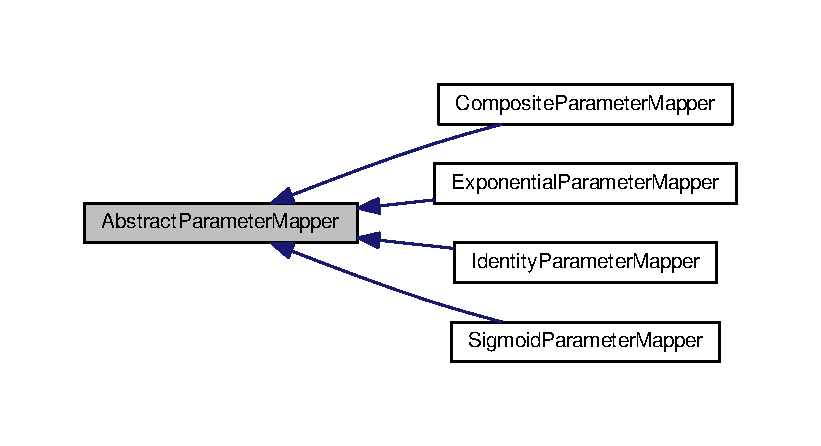
\includegraphics[width=350pt]{classAbstractParameterMapper__inherit__graph}
\end{center}
\end{figure}
\subsection*{Public Member Functions}
\begin{DoxyCompactItemize}
\item 
\mbox{\hyperlink{classAbstractParameterMapper_ae8e7c815952e44d47bc406f396fdf0d6}{Abstract\+Parameter\+Mapper}} ()
\item 
virtual vector$<$ double $>$ \mbox{\hyperlink{classAbstractParameterMapper_abb9e78545ff023f2b786b759ec2d23e4}{map}} (vector$<$ double $>$ problem\+Parameter)=0
\item 
virtual vector$<$ double $>$ \mbox{\hyperlink{classAbstractParameterMapper_a7fc9715759582e218a3bc38ec43e2d57}{unmap}} (vector$<$ double $>$ kalman\+Parameter)=0
\end{DoxyCompactItemize}


\subsection{Detailed Description}
Abstract class that model the functions required for a parameters mapping function. The mapping functions will map the problem parameters into a better-\/behaved space of parameter for the kalman optimization. The map and unmap functions are inverse one to other. 

Definition at line 21 of file Abstract\+Parameter\+Mapper.\+h.



\subsection{Constructor \& Destructor Documentation}
\mbox{\Hypertarget{classAbstractParameterMapper_ae8e7c815952e44d47bc406f396fdf0d6}\label{classAbstractParameterMapper_ae8e7c815952e44d47bc406f396fdf0d6}} 
\index{Abstract\+Parameter\+Mapper@{Abstract\+Parameter\+Mapper}!Abstract\+Parameter\+Mapper@{Abstract\+Parameter\+Mapper}}
\index{Abstract\+Parameter\+Mapper@{Abstract\+Parameter\+Mapper}!Abstract\+Parameter\+Mapper@{Abstract\+Parameter\+Mapper}}
\subsubsection{\texorpdfstring{Abstract\+Parameter\+Mapper()}{AbstractParameterMapper()}}
{\footnotesize\ttfamily Abstract\+Parameter\+Mapper\+::\+Abstract\+Parameter\+Mapper (\begin{DoxyParamCaption}{ }\end{DoxyParamCaption})}

Dummy constructor. 

Definition at line 10 of file Abstract\+Parameter\+Mapper.\+cpp.



\subsection{Member Function Documentation}
\mbox{\Hypertarget{classAbstractParameterMapper_abb9e78545ff023f2b786b759ec2d23e4}\label{classAbstractParameterMapper_abb9e78545ff023f2b786b759ec2d23e4}} 
\index{Abstract\+Parameter\+Mapper@{Abstract\+Parameter\+Mapper}!map@{map}}
\index{map@{map}!Abstract\+Parameter\+Mapper@{Abstract\+Parameter\+Mapper}}
\subsubsection{\texorpdfstring{map()}{map()}}
{\footnotesize\ttfamily virtual vector$<$double$>$ Abstract\+Parameter\+Mapper\+::map (\begin{DoxyParamCaption}\item[{vector$<$ double $>$}]{problem\+Parameter }\end{DoxyParamCaption})\hspace{0.3cm}{\ttfamily [pure virtual]}}

Maps the problem parameters into the space of parameters where kalman filter optimize them. 
\begin{DoxyParams}{Parameters}
{\em problem\+Parameter} & Set of problem parameters. \\
\hline
\end{DoxyParams}
\begin{DoxyReturn}{Returns}
Set of kalman parameters 
\end{DoxyReturn}


Implemented in \mbox{\hyperlink{classCompositeParameterMapper_abac90f20835ad311cfdfc952956b9624}{Composite\+Parameter\+Mapper}}, \mbox{\hyperlink{classSigmoidParameterMapper_a808db49587ff6c2d2c2b2efc84de80f6}{Sigmoid\+Parameter\+Mapper}}, \mbox{\hyperlink{classExponentialParameterMapper_a6abcf5b0efb8ef01ced062b7498c923e}{Exponential\+Parameter\+Mapper}}, and \mbox{\hyperlink{classIdentityParameterMapper_a21105fcfd2e89ac5529f97433f03b1c3}{Identity\+Parameter\+Mapper}}.

\mbox{\Hypertarget{classAbstractParameterMapper_a7fc9715759582e218a3bc38ec43e2d57}\label{classAbstractParameterMapper_a7fc9715759582e218a3bc38ec43e2d57}} 
\index{Abstract\+Parameter\+Mapper@{Abstract\+Parameter\+Mapper}!unmap@{unmap}}
\index{unmap@{unmap}!Abstract\+Parameter\+Mapper@{Abstract\+Parameter\+Mapper}}
\subsubsection{\texorpdfstring{unmap()}{unmap()}}
{\footnotesize\ttfamily virtual vector$<$double$>$ Abstract\+Parameter\+Mapper\+::unmap (\begin{DoxyParamCaption}\item[{vector$<$ double $>$}]{kalman\+Parameter }\end{DoxyParamCaption})\hspace{0.3cm}{\ttfamily [pure virtual]}}

Maps the kalman parameters into the space of problem parameters. 
\begin{DoxyParams}{Parameters}
{\em kalman\+Parameter} & Set of kalman parameters. \\
\hline
\end{DoxyParams}
\begin{DoxyReturn}{Returns}
Set of problem parameters. 
\end{DoxyReturn}


Implemented in \mbox{\hyperlink{classCompositeParameterMapper_a15d15009cf9026b22f27f5d8a5880a4e}{Composite\+Parameter\+Mapper}}, \mbox{\hyperlink{classSigmoidParameterMapper_a5b7031c2945f69130e0423427525e256}{Sigmoid\+Parameter\+Mapper}}, \mbox{\hyperlink{classExponentialParameterMapper_ad7040a1ac834e53691bd157df925c545}{Exponential\+Parameter\+Mapper}}, and \mbox{\hyperlink{classIdentityParameterMapper_ad7ad11e683701104024a553eb8f2373b}{Identity\+Parameter\+Mapper}}.



The documentation for this class was generated from the following files\+:\begin{DoxyCompactItemize}
\item 
mapping/Abstract\+Parameter\+Mapper.\+h\item 
mapping/Abstract\+Parameter\+Mapper.\+cpp\end{DoxyCompactItemize}

\hypertarget{classAbstractROUKF}{}\section{Abstract\+R\+O\+U\+KF Class Reference}
\label{classAbstractROUKF}\index{Abstract\+R\+O\+U\+KF@{Abstract\+R\+O\+U\+KF}}


Inheritance diagram for Abstract\+R\+O\+U\+KF\+:\nopagebreak
\begin{figure}[H]
\begin{center}
\leavevmode
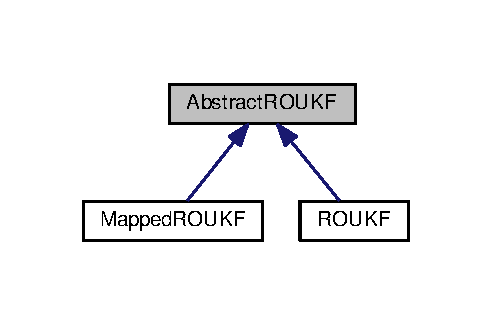
\includegraphics[width=236pt]{classAbstractROUKF__inherit__graph}
\end{center}
\end{figure}
\subsection*{Public Member Functions}
\begin{DoxyCompactItemize}
\item 
\mbox{\hyperlink{classAbstractROUKF_afbeabf5f80a3cd9dcbd9c551cde20cfe}{Abstract\+R\+O\+U\+KF}} ()
\item 
virtual \mbox{\hyperlink{classAbstractROUKF_a6b02fbadd6db005bb85fc364fbe5d7f9}{$\sim$\+Abstract\+R\+O\+U\+KF}} ()
\item 
void \mbox{\hyperlink{classAbstractROUKF_a663975374b647bd1ce1b4dc54e937de9}{to\+String}} ()
\item 
bool \mbox{\hyperlink{classAbstractROUKF_a7f9deb98273cfc2282e2902cdf716bff}{has\+Converged}} (bool is\+Convergence\+Relative)
\item 
vector$<$ double $>$ \mbox{\hyperlink{classAbstractROUKF_a210b89fa43dd6c6f658518d24dcc9c9c}{get\+Parameters\+Std}} ()
\item 
void \mbox{\hyperlink{classAbstractROUKF_ad24dafa1f4cb02a38958264740588b87}{get\+State}} (double $\ast$$\ast$XC)
\item 
void \mbox{\hyperlink{classAbstractROUKF_a618f4719892c0997e5f62cc23913aa12}{set\+State}} (double $\ast$XC)
\item 
virtual void \mbox{\hyperlink{classAbstractROUKF_a1fa0b3e17f2618789dca9319bd755830}{get\+Parameters}} (double $\ast$$\ast$ThetaC)
\item 
virtual void \mbox{\hyperlink{classAbstractROUKF_a8e8f7c34007a2363530f7cca4cfb0c9f}{set\+Parameters}} (double $\ast$ThetaC)
\item 
void \mbox{\hyperlink{classAbstractROUKF_aff309e6f34502fe604b1130a4185cb56}{get\+Error}} (double $\ast$$\ast$err)
\item 
double \mbox{\hyperlink{classAbstractROUKF_ae3daccd71ef910705d340567a22abdff}{get\+Obs\+Error}} (int num\+Observation)
\item 
int \mbox{\hyperlink{classAbstractROUKF_af26c89f7ed4191cbf41d945808d0daee}{get\+Observations}} () const
\item 
int \mbox{\hyperlink{classAbstractROUKF_a904fa28784c0bf5ed96502b6bea74346}{get\+States}} () const
\item 
double \mbox{\hyperlink{classAbstractROUKF_ac1d872b69fb061600b259d13b2add657}{get\+Max\+Iterations}} () const
\item 
void \mbox{\hyperlink{classAbstractROUKF_affbf7bade0ebe7441377f88e6461e84f}{set\+Max\+Iterations}} (double \mbox{\hyperlink{classAbstractROUKF_a268b49ab648ee8013b15ef5127d4fef1}{max\+Iterations}})
\item 
double \mbox{\hyperlink{classAbstractROUKF_a408197857ee4f8084170a8240db1eb29}{get\+Tolerance}} () const
\item 
void \mbox{\hyperlink{classAbstractROUKF_afc0c756daaba8dbaa4da1e38c97a16e2}{set\+Tolerance}} (double \mbox{\hyperlink{classAbstractROUKF_aecf6562ecf3ea0bef0d4875cae682b11}{tolerance}})
\end{DoxyCompactItemize}
\subsection*{Protected Attributes}
\begin{DoxyCompactItemize}
\item 
arma\+::mat \mbox{\hyperlink{classAbstractROUKF_afdb4deed00416489ced1729c22a317f2}{X}}
\item 
arma\+::mat \mbox{\hyperlink{classAbstractROUKF_a09460cd2349481e27e68718f47ad354b}{Theta}}
\item 
arma\+::mat \mbox{\hyperlink{classAbstractROUKF_a750d4ddf5b83c1ecd319a6b1a8f9ffb5}{U}}
\item 
arma\+::mat \mbox{\hyperlink{classAbstractROUKF_a98dd192be29bfa224abb3fe21f60ac92}{U2}}
\item 
arma\+::mat \mbox{\hyperlink{classAbstractROUKF_a5dfab9d5823117885e01db2e591eeb59}{LX}}
\item 
arma\+::mat \mbox{\hyperlink{classAbstractROUKF_a5c4be89d8f4d3c6ce73e05242bbd1d5e}{L\+Theta}}
\item 
arma\+::sp\+\_\+mat \mbox{\hyperlink{classAbstractROUKF_a0bb579dc353724d64ce50df76b5ecacb}{Wi}}
\item 
arma\+::mat \mbox{\hyperlink{classAbstractROUKF_a1d02b594a134c2644c0b64889c9ab34a}{sigma}}
\item 
arma\+::mat \mbox{\hyperlink{classAbstractROUKF_a7f0b59c793a213079124cfce6284e58c}{Dsigma}}
\item 
arma\+::mat \mbox{\hyperlink{classAbstractROUKF_ab3c7c4f238cedee2784a450cd10eb98b}{Pa}}
\item 
arma\+::mat \mbox{\hyperlink{classAbstractROUKF_a551d0b61b010efe7923358c93cbd0db5}{error}}
\item 
int \mbox{\hyperlink{classAbstractROUKF_a4f6403f7fd2fac691e4ac516f47c0a06}{n\+Observations}}
\item 
int \mbox{\hyperlink{classAbstractROUKF_a488f708dcdd66758cd879421cd454846}{n\+Parameters}}
\item 
int \mbox{\hyperlink{classAbstractROUKF_af9ce480feb5d97761f20fdd546878aff}{n\+States}}
\item 
double \mbox{\hyperlink{classAbstractROUKF_ada380355583bc96844c1f1bb0e202a40}{alpha}}
\item 
double \mbox{\hyperlink{classAbstractROUKF_aecf6562ecf3ea0bef0d4875cae682b11}{tolerance}}
\item 
double \mbox{\hyperlink{classAbstractROUKF_a268b49ab648ee8013b15ef5127d4fef1}{max\+Iterations}}
\item 
double \mbox{\hyperlink{classAbstractROUKF_a699ef3cc8c3c5fa650d065e6dd77e12a}{prev\+Error}}
\item 
double \mbox{\hyperlink{classAbstractROUKF_aaf3e4ce3407d3ca6ad1b06ba2592a6ce}{curr\+Error}}
\item 
long long int \mbox{\hyperlink{classAbstractROUKF_a8e7ff4187e5808a032fd97d1b8a024b3}{curr\+It}}
\end{DoxyCompactItemize}


\subsection{Detailed Description}


Definition at line 28 of file Abstract\+R\+O\+U\+K\+F.\+h.



\subsection{Constructor \& Destructor Documentation}
\mbox{\Hypertarget{classAbstractROUKF_afbeabf5f80a3cd9dcbd9c551cde20cfe}\label{classAbstractROUKF_afbeabf5f80a3cd9dcbd9c551cde20cfe}} 
\index{Abstract\+R\+O\+U\+KF@{Abstract\+R\+O\+U\+KF}!Abstract\+R\+O\+U\+KF@{Abstract\+R\+O\+U\+KF}}
\index{Abstract\+R\+O\+U\+KF@{Abstract\+R\+O\+U\+KF}!Abstract\+R\+O\+U\+KF@{Abstract\+R\+O\+U\+KF}}
\subsubsection{\texorpdfstring{Abstract\+R\+O\+U\+K\+F()}{AbstractROUKF()}}
{\footnotesize\ttfamily Abstract\+R\+O\+U\+K\+F\+::\+Abstract\+R\+O\+U\+KF (\begin{DoxyParamCaption}{ }\end{DoxyParamCaption})}

Abstract constructor. 

Definition at line 10 of file Abstract\+R\+O\+U\+K\+F.\+cpp.

\mbox{\Hypertarget{classAbstractROUKF_a6b02fbadd6db005bb85fc364fbe5d7f9}\label{classAbstractROUKF_a6b02fbadd6db005bb85fc364fbe5d7f9}} 
\index{Abstract\+R\+O\+U\+KF@{Abstract\+R\+O\+U\+KF}!````~Abstract\+R\+O\+U\+KF@{$\sim$\+Abstract\+R\+O\+U\+KF}}
\index{````~Abstract\+R\+O\+U\+KF@{$\sim$\+Abstract\+R\+O\+U\+KF}!Abstract\+R\+O\+U\+KF@{Abstract\+R\+O\+U\+KF}}
\subsubsection{\texorpdfstring{$\sim$\+Abstract\+R\+O\+U\+K\+F()}{~AbstractROUKF()}}
{\footnotesize\ttfamily Abstract\+R\+O\+U\+K\+F\+::$\sim$\+Abstract\+R\+O\+U\+KF (\begin{DoxyParamCaption}{ }\end{DoxyParamCaption})\hspace{0.3cm}{\ttfamily [virtual]}}

Virtual destructor. 

Definition at line 16 of file Abstract\+R\+O\+U\+K\+F.\+cpp.



\subsection{Member Function Documentation}
\mbox{\Hypertarget{classAbstractROUKF_aff309e6f34502fe604b1130a4185cb56}\label{classAbstractROUKF_aff309e6f34502fe604b1130a4185cb56}} 
\index{Abstract\+R\+O\+U\+KF@{Abstract\+R\+O\+U\+KF}!get\+Error@{get\+Error}}
\index{get\+Error@{get\+Error}!Abstract\+R\+O\+U\+KF@{Abstract\+R\+O\+U\+KF}}
\subsubsection{\texorpdfstring{get\+Error()}{getError()}}
{\footnotesize\ttfamily void Abstract\+R\+O\+U\+K\+F\+::get\+Error (\begin{DoxyParamCaption}\item[{double $\ast$$\ast$}]{err }\end{DoxyParamCaption})}

Returns the error associated to each observation at the current iteration in a S\+TL array. 
\begin{DoxyParams}{Parameters}
{\em err} & Error associated to each observation at the current iteration. \\
\hline
\end{DoxyParams}


Definition at line 35 of file Abstract\+R\+O\+U\+K\+F.\+cpp.

\mbox{\Hypertarget{classAbstractROUKF_ac1d872b69fb061600b259d13b2add657}\label{classAbstractROUKF_ac1d872b69fb061600b259d13b2add657}} 
\index{Abstract\+R\+O\+U\+KF@{Abstract\+R\+O\+U\+KF}!get\+Max\+Iterations@{get\+Max\+Iterations}}
\index{get\+Max\+Iterations@{get\+Max\+Iterations}!Abstract\+R\+O\+U\+KF@{Abstract\+R\+O\+U\+KF}}
\subsubsection{\texorpdfstring{get\+Max\+Iterations()}{getMaxIterations()}}
{\footnotesize\ttfamily double Abstract\+R\+O\+U\+K\+F\+::get\+Max\+Iterations (\begin{DoxyParamCaption}{ }\end{DoxyParamCaption}) const}

Getter of the field {\ttfamily max\+Iterations}. \begin{DoxyReturn}{Returns}
Field {\ttfamily max\+Iterations}. 
\end{DoxyReturn}


Definition at line 72 of file Abstract\+R\+O\+U\+K\+F.\+cpp.

\mbox{\Hypertarget{classAbstractROUKF_ae3daccd71ef910705d340567a22abdff}\label{classAbstractROUKF_ae3daccd71ef910705d340567a22abdff}} 
\index{Abstract\+R\+O\+U\+KF@{Abstract\+R\+O\+U\+KF}!get\+Obs\+Error@{get\+Obs\+Error}}
\index{get\+Obs\+Error@{get\+Obs\+Error}!Abstract\+R\+O\+U\+KF@{Abstract\+R\+O\+U\+KF}}
\subsubsection{\texorpdfstring{get\+Obs\+Error()}{getObsError()}}
{\footnotesize\ttfamily double Abstract\+R\+O\+U\+K\+F\+::get\+Obs\+Error (\begin{DoxyParamCaption}\item[{int}]{num\+Observation }\end{DoxyParamCaption})}

Returns the error associated to the {\ttfamily num\+Observation} observation. 
\begin{DoxyParams}{Parameters}
{\em num\+Observation} & Index of the observation of interest. \\
\hline
\end{DoxyParams}


Definition at line 39 of file Abstract\+R\+O\+U\+K\+F.\+cpp.

\mbox{\Hypertarget{classAbstractROUKF_af26c89f7ed4191cbf41d945808d0daee}\label{classAbstractROUKF_af26c89f7ed4191cbf41d945808d0daee}} 
\index{Abstract\+R\+O\+U\+KF@{Abstract\+R\+O\+U\+KF}!get\+Observations@{get\+Observations}}
\index{get\+Observations@{get\+Observations}!Abstract\+R\+O\+U\+KF@{Abstract\+R\+O\+U\+KF}}
\subsubsection{\texorpdfstring{get\+Observations()}{getObservations()}}
{\footnotesize\ttfamily int Abstract\+R\+O\+U\+K\+F\+::get\+Observations (\begin{DoxyParamCaption}{ }\end{DoxyParamCaption}) const}

Return the number of observations used in this instance of the kalman filter. \begin{DoxyReturn}{Returns}
Number of observations used in this instance of the kalman filter. 
\end{DoxyReturn}


Definition at line 62 of file Abstract\+R\+O\+U\+K\+F.\+cpp.

\mbox{\Hypertarget{classAbstractROUKF_a1fa0b3e17f2618789dca9319bd755830}\label{classAbstractROUKF_a1fa0b3e17f2618789dca9319bd755830}} 
\index{Abstract\+R\+O\+U\+KF@{Abstract\+R\+O\+U\+KF}!get\+Parameters@{get\+Parameters}}
\index{get\+Parameters@{get\+Parameters}!Abstract\+R\+O\+U\+KF@{Abstract\+R\+O\+U\+KF}}
\subsubsection{\texorpdfstring{get\+Parameters()}{getParameters()}}
{\footnotesize\ttfamily void Abstract\+R\+O\+U\+K\+F\+::get\+Parameters (\begin{DoxyParamCaption}\item[{double $\ast$$\ast$}]{ThetaC }\end{DoxyParamCaption})\hspace{0.3cm}{\ttfamily [virtual]}}

Getter of the field {\ttfamily Theta}. 
\begin{DoxyParams}{Parameters}
{\em ThetaC} & Field {\ttfamily Theta} converted to S\+TL array. \\
\hline
\end{DoxyParams}


Reimplemented in \mbox{\hyperlink{classMappedROUKF_aa6670e2cc9899b93b71db3f238ae93f3}{Mapped\+R\+O\+U\+KF}}.



Definition at line 19 of file Abstract\+R\+O\+U\+K\+F.\+cpp.

\mbox{\Hypertarget{classAbstractROUKF_a210b89fa43dd6c6f658518d24dcc9c9c}\label{classAbstractROUKF_a210b89fa43dd6c6f658518d24dcc9c9c}} 
\index{Abstract\+R\+O\+U\+KF@{Abstract\+R\+O\+U\+KF}!get\+Parameters\+Std@{get\+Parameters\+Std}}
\index{get\+Parameters\+Std@{get\+Parameters\+Std}!Abstract\+R\+O\+U\+KF@{Abstract\+R\+O\+U\+KF}}
\subsubsection{\texorpdfstring{get\+Parameters\+Std()}{getParametersStd()}}
{\footnotesize\ttfamily vector$<$ double $>$ Abstract\+R\+O\+U\+K\+F\+::get\+Parameters\+Std (\begin{DoxyParamCaption}{ }\end{DoxyParamCaption})}

Returns a vector with the standard variation of each parameter at the current iteration. \begin{DoxyReturn}{Returns}
Vector with the standard variation of each parameter at the current iteration. 
\end{DoxyReturn}


Definition at line 57 of file Abstract\+R\+O\+U\+K\+F.\+cpp.

\mbox{\Hypertarget{classAbstractROUKF_ad24dafa1f4cb02a38958264740588b87}\label{classAbstractROUKF_ad24dafa1f4cb02a38958264740588b87}} 
\index{Abstract\+R\+O\+U\+KF@{Abstract\+R\+O\+U\+KF}!get\+State@{get\+State}}
\index{get\+State@{get\+State}!Abstract\+R\+O\+U\+KF@{Abstract\+R\+O\+U\+KF}}
\subsubsection{\texorpdfstring{get\+State()}{getState()}}
{\footnotesize\ttfamily void Abstract\+R\+O\+U\+K\+F\+::get\+State (\begin{DoxyParamCaption}\item[{double $\ast$$\ast$}]{XC }\end{DoxyParamCaption})}

Getter of the field {\ttfamily X}. 
\begin{DoxyParams}{Parameters}
{\em XC} & Field {\ttfamily X} converted to S\+TL array. \\
\hline
\end{DoxyParams}


Definition at line 27 of file Abstract\+R\+O\+U\+K\+F.\+cpp.

\mbox{\Hypertarget{classAbstractROUKF_a904fa28784c0bf5ed96502b6bea74346}\label{classAbstractROUKF_a904fa28784c0bf5ed96502b6bea74346}} 
\index{Abstract\+R\+O\+U\+KF@{Abstract\+R\+O\+U\+KF}!get\+States@{get\+States}}
\index{get\+States@{get\+States}!Abstract\+R\+O\+U\+KF@{Abstract\+R\+O\+U\+KF}}
\subsubsection{\texorpdfstring{get\+States()}{getStates()}}
{\footnotesize\ttfamily int Abstract\+R\+O\+U\+K\+F\+::get\+States (\begin{DoxyParamCaption}{ }\end{DoxyParamCaption}) const}

Return the number of states used in this instance of the kalman filter. \begin{DoxyReturn}{Returns}
Number of states used in this instance of the kalman filter. 
\end{DoxyReturn}


Definition at line 67 of file Abstract\+R\+O\+U\+K\+F.\+cpp.

\mbox{\Hypertarget{classAbstractROUKF_a408197857ee4f8084170a8240db1eb29}\label{classAbstractROUKF_a408197857ee4f8084170a8240db1eb29}} 
\index{Abstract\+R\+O\+U\+KF@{Abstract\+R\+O\+U\+KF}!get\+Tolerance@{get\+Tolerance}}
\index{get\+Tolerance@{get\+Tolerance}!Abstract\+R\+O\+U\+KF@{Abstract\+R\+O\+U\+KF}}
\subsubsection{\texorpdfstring{get\+Tolerance()}{getTolerance()}}
{\footnotesize\ttfamily double Abstract\+R\+O\+U\+K\+F\+::get\+Tolerance (\begin{DoxyParamCaption}{ }\end{DoxyParamCaption}) const}

Getter of the field {\ttfamily tolerance}. \begin{DoxyReturn}{Returns}
Field {\ttfamily tolerance}. 
\end{DoxyReturn}


Definition at line 82 of file Abstract\+R\+O\+U\+K\+F.\+cpp.

\mbox{\Hypertarget{classAbstractROUKF_a7f9deb98273cfc2282e2902cdf716bff}\label{classAbstractROUKF_a7f9deb98273cfc2282e2902cdf716bff}} 
\index{Abstract\+R\+O\+U\+KF@{Abstract\+R\+O\+U\+KF}!has\+Converged@{has\+Converged}}
\index{has\+Converged@{has\+Converged}!Abstract\+R\+O\+U\+KF@{Abstract\+R\+O\+U\+KF}}
\subsubsection{\texorpdfstring{has\+Converged()}{hasConverged()}}
{\footnotesize\ttfamily bool Abstract\+R\+O\+U\+K\+F\+::has\+Converged (\begin{DoxyParamCaption}\item[{bool}]{is\+Convergence\+Relative }\end{DoxyParamCaption})}

Return if the filter has converged according to the specified {\ttfamily tolerance}. 
\begin{DoxyParams}{Parameters}
{\em is\+Convergence\+Relative} & If the convergence is relative or absolute. \\
\hline
\end{DoxyParams}
\begin{DoxyReturn}{Returns}
If it is converged. 
\end{DoxyReturn}


Definition at line 92 of file Abstract\+R\+O\+U\+K\+F.\+cpp.

\mbox{\Hypertarget{classAbstractROUKF_affbf7bade0ebe7441377f88e6461e84f}\label{classAbstractROUKF_affbf7bade0ebe7441377f88e6461e84f}} 
\index{Abstract\+R\+O\+U\+KF@{Abstract\+R\+O\+U\+KF}!set\+Max\+Iterations@{set\+Max\+Iterations}}
\index{set\+Max\+Iterations@{set\+Max\+Iterations}!Abstract\+R\+O\+U\+KF@{Abstract\+R\+O\+U\+KF}}
\subsubsection{\texorpdfstring{set\+Max\+Iterations()}{setMaxIterations()}}
{\footnotesize\ttfamily void Abstract\+R\+O\+U\+K\+F\+::set\+Max\+Iterations (\begin{DoxyParamCaption}\item[{double}]{max\+Iterations }\end{DoxyParamCaption})}

Setter of the field {\ttfamily max\+Iterations}. 
\begin{DoxyParams}{Parameters}
{\em max\+Iterations} & Maximum number of iterations. \\
\hline
\end{DoxyParams}


Definition at line 77 of file Abstract\+R\+O\+U\+K\+F.\+cpp.

\mbox{\Hypertarget{classAbstractROUKF_a8e8f7c34007a2363530f7cca4cfb0c9f}\label{classAbstractROUKF_a8e8f7c34007a2363530f7cca4cfb0c9f}} 
\index{Abstract\+R\+O\+U\+KF@{Abstract\+R\+O\+U\+KF}!set\+Parameters@{set\+Parameters}}
\index{set\+Parameters@{set\+Parameters}!Abstract\+R\+O\+U\+KF@{Abstract\+R\+O\+U\+KF}}
\subsubsection{\texorpdfstring{set\+Parameters()}{setParameters()}}
{\footnotesize\ttfamily void Abstract\+R\+O\+U\+K\+F\+::set\+Parameters (\begin{DoxyParamCaption}\item[{double $\ast$}]{ThetaC }\end{DoxyParamCaption})\hspace{0.3cm}{\ttfamily [virtual]}}

Setter of the field {\ttfamily Theta}. 
\begin{DoxyParams}{Parameters}
{\em ThetaC} & Array of parameters. \\
\hline
\end{DoxyParams}


Reimplemented in \mbox{\hyperlink{classMappedROUKF_a4d3a109dc95812c8d9c6ac2a489349c2}{Mapped\+R\+O\+U\+KF}}.



Definition at line 23 of file Abstract\+R\+O\+U\+K\+F.\+cpp.

\mbox{\Hypertarget{classAbstractROUKF_a618f4719892c0997e5f62cc23913aa12}\label{classAbstractROUKF_a618f4719892c0997e5f62cc23913aa12}} 
\index{Abstract\+R\+O\+U\+KF@{Abstract\+R\+O\+U\+KF}!set\+State@{set\+State}}
\index{set\+State@{set\+State}!Abstract\+R\+O\+U\+KF@{Abstract\+R\+O\+U\+KF}}
\subsubsection{\texorpdfstring{set\+State()}{setState()}}
{\footnotesize\ttfamily void Abstract\+R\+O\+U\+K\+F\+::set\+State (\begin{DoxyParamCaption}\item[{double $\ast$}]{XC }\end{DoxyParamCaption})}

Setter of the field {\ttfamily X}. 
\begin{DoxyParams}{Parameters}
{\em XC} & Array of states. \\
\hline
\end{DoxyParams}


Definition at line 31 of file Abstract\+R\+O\+U\+K\+F.\+cpp.

\mbox{\Hypertarget{classAbstractROUKF_afc0c756daaba8dbaa4da1e38c97a16e2}\label{classAbstractROUKF_afc0c756daaba8dbaa4da1e38c97a16e2}} 
\index{Abstract\+R\+O\+U\+KF@{Abstract\+R\+O\+U\+KF}!set\+Tolerance@{set\+Tolerance}}
\index{set\+Tolerance@{set\+Tolerance}!Abstract\+R\+O\+U\+KF@{Abstract\+R\+O\+U\+KF}}
\subsubsection{\texorpdfstring{set\+Tolerance()}{setTolerance()}}
{\footnotesize\ttfamily void Abstract\+R\+O\+U\+K\+F\+::set\+Tolerance (\begin{DoxyParamCaption}\item[{double}]{tolerance }\end{DoxyParamCaption})}

Setter of the field {\ttfamily tolerance}. 
\begin{DoxyParams}{Parameters}
{\em tolerance} & Maximum tolerance allowed. \\
\hline
\end{DoxyParams}


Definition at line 87 of file Abstract\+R\+O\+U\+K\+F.\+cpp.

\mbox{\Hypertarget{classAbstractROUKF_a663975374b647bd1ce1b4dc54e937de9}\label{classAbstractROUKF_a663975374b647bd1ce1b4dc54e937de9}} 
\index{Abstract\+R\+O\+U\+KF@{Abstract\+R\+O\+U\+KF}!to\+String@{to\+String}}
\index{to\+String@{to\+String}!Abstract\+R\+O\+U\+KF@{Abstract\+R\+O\+U\+KF}}
\subsubsection{\texorpdfstring{to\+String()}{toString()}}
{\footnotesize\ttfamily void Abstract\+R\+O\+U\+K\+F\+::to\+String (\begin{DoxyParamCaption}{ }\end{DoxyParamCaption})}

Prints the private attributes of the \mbox{\hyperlink{classROUKF}{R\+O\+U\+KF}} instance. 

Definition at line 43 of file Abstract\+R\+O\+U\+K\+F.\+cpp.



\subsection{Member Data Documentation}
\mbox{\Hypertarget{classAbstractROUKF_ada380355583bc96844c1f1bb0e202a40}\label{classAbstractROUKF_ada380355583bc96844c1f1bb0e202a40}} 
\index{Abstract\+R\+O\+U\+KF@{Abstract\+R\+O\+U\+KF}!alpha@{alpha}}
\index{alpha@{alpha}!Abstract\+R\+O\+U\+KF@{Abstract\+R\+O\+U\+KF}}
\subsubsection{\texorpdfstring{alpha}{alpha}}
{\footnotesize\ttfamily double Abstract\+R\+O\+U\+K\+F\+::alpha\hspace{0.3cm}{\ttfamily [protected]}}

Weight for each sigma point. 

Definition at line 63 of file Abstract\+R\+O\+U\+K\+F.\+h.

\mbox{\Hypertarget{classAbstractROUKF_aaf3e4ce3407d3ca6ad1b06ba2592a6ce}\label{classAbstractROUKF_aaf3e4ce3407d3ca6ad1b06ba2592a6ce}} 
\index{Abstract\+R\+O\+U\+KF@{Abstract\+R\+O\+U\+KF}!curr\+Error@{curr\+Error}}
\index{curr\+Error@{curr\+Error}!Abstract\+R\+O\+U\+KF@{Abstract\+R\+O\+U\+KF}}
\subsubsection{\texorpdfstring{curr\+Error}{currError}}
{\footnotesize\ttfamily double Abstract\+R\+O\+U\+K\+F\+::curr\+Error\hspace{0.3cm}{\ttfamily [protected]}}

Current iteration error. 

Definition at line 72 of file Abstract\+R\+O\+U\+K\+F.\+h.

\mbox{\Hypertarget{classAbstractROUKF_a8e7ff4187e5808a032fd97d1b8a024b3}\label{classAbstractROUKF_a8e7ff4187e5808a032fd97d1b8a024b3}} 
\index{Abstract\+R\+O\+U\+KF@{Abstract\+R\+O\+U\+KF}!curr\+It@{curr\+It}}
\index{curr\+It@{curr\+It}!Abstract\+R\+O\+U\+KF@{Abstract\+R\+O\+U\+KF}}
\subsubsection{\texorpdfstring{curr\+It}{currIt}}
{\footnotesize\ttfamily long long int Abstract\+R\+O\+U\+K\+F\+::curr\+It\hspace{0.3cm}{\ttfamily [protected]}}

Current iteration. 

Definition at line 74 of file Abstract\+R\+O\+U\+K\+F.\+h.

\mbox{\Hypertarget{classAbstractROUKF_a7f0b59c793a213079124cfce6284e58c}\label{classAbstractROUKF_a7f0b59c793a213079124cfce6284e58c}} 
\index{Abstract\+R\+O\+U\+KF@{Abstract\+R\+O\+U\+KF}!Dsigma@{Dsigma}}
\index{Dsigma@{Dsigma}!Abstract\+R\+O\+U\+KF@{Abstract\+R\+O\+U\+KF}}
\subsubsection{\texorpdfstring{Dsigma}{Dsigma}}
{\footnotesize\ttfamily arma\+::mat Abstract\+R\+O\+U\+K\+F\+::\+Dsigma\hspace{0.3cm}{\ttfamily [protected]}}

Matrix with sigma points weighted as rows. 

Definition at line 49 of file Abstract\+R\+O\+U\+K\+F.\+h.

\mbox{\Hypertarget{classAbstractROUKF_a551d0b61b010efe7923358c93cbd0db5}\label{classAbstractROUKF_a551d0b61b010efe7923358c93cbd0db5}} 
\index{Abstract\+R\+O\+U\+KF@{Abstract\+R\+O\+U\+KF}!error@{error}}
\index{error@{error}!Abstract\+R\+O\+U\+KF@{Abstract\+R\+O\+U\+KF}}
\subsubsection{\texorpdfstring{error}{error}}
{\footnotesize\ttfamily arma\+::mat Abstract\+R\+O\+U\+K\+F\+::error\hspace{0.3cm}{\ttfamily [protected]}}

Vector with the observations errors after the last iteration. 

Definition at line 54 of file Abstract\+R\+O\+U\+K\+F.\+h.

\mbox{\Hypertarget{classAbstractROUKF_a5c4be89d8f4d3c6ce73e05242bbd1d5e}\label{classAbstractROUKF_a5c4be89d8f4d3c6ce73e05242bbd1d5e}} 
\index{Abstract\+R\+O\+U\+KF@{Abstract\+R\+O\+U\+KF}!L\+Theta@{L\+Theta}}
\index{L\+Theta@{L\+Theta}!Abstract\+R\+O\+U\+KF@{Abstract\+R\+O\+U\+KF}}
\subsubsection{\texorpdfstring{L\+Theta}{LTheta}}
{\footnotesize\ttfamily arma\+::mat Abstract\+R\+O\+U\+K\+F\+::\+L\+Theta\hspace{0.3cm}{\ttfamily [protected]}}

L part of the covariance matrix after LU factorization concerning to the parameter part of the extended state vector. 

Definition at line 42 of file Abstract\+R\+O\+U\+K\+F.\+h.

\mbox{\Hypertarget{classAbstractROUKF_a5dfab9d5823117885e01db2e591eeb59}\label{classAbstractROUKF_a5dfab9d5823117885e01db2e591eeb59}} 
\index{Abstract\+R\+O\+U\+KF@{Abstract\+R\+O\+U\+KF}!LX@{LX}}
\index{LX@{LX}!Abstract\+R\+O\+U\+KF@{Abstract\+R\+O\+U\+KF}}
\subsubsection{\texorpdfstring{LX}{LX}}
{\footnotesize\ttfamily arma\+::mat Abstract\+R\+O\+U\+K\+F\+::\+LX\hspace{0.3cm}{\ttfamily [protected]}}

L part of the covariance matrix after LU factorization concerning to the state part of the extended state vector. 

Definition at line 40 of file Abstract\+R\+O\+U\+K\+F.\+h.

\mbox{\Hypertarget{classAbstractROUKF_a268b49ab648ee8013b15ef5127d4fef1}\label{classAbstractROUKF_a268b49ab648ee8013b15ef5127d4fef1}} 
\index{Abstract\+R\+O\+U\+KF@{Abstract\+R\+O\+U\+KF}!max\+Iterations@{max\+Iterations}}
\index{max\+Iterations@{max\+Iterations}!Abstract\+R\+O\+U\+KF@{Abstract\+R\+O\+U\+KF}}
\subsubsection{\texorpdfstring{max\+Iterations}{maxIterations}}
{\footnotesize\ttfamily double Abstract\+R\+O\+U\+K\+F\+::max\+Iterations\hspace{0.3cm}{\ttfamily [protected]}}

Maximum number of iterations. 

Definition at line 68 of file Abstract\+R\+O\+U\+K\+F.\+h.

\mbox{\Hypertarget{classAbstractROUKF_a4f6403f7fd2fac691e4ac516f47c0a06}\label{classAbstractROUKF_a4f6403f7fd2fac691e4ac516f47c0a06}} 
\index{Abstract\+R\+O\+U\+KF@{Abstract\+R\+O\+U\+KF}!n\+Observations@{n\+Observations}}
\index{n\+Observations@{n\+Observations}!Abstract\+R\+O\+U\+KF@{Abstract\+R\+O\+U\+KF}}
\subsubsection{\texorpdfstring{n\+Observations}{nObservations}}
{\footnotesize\ttfamily int Abstract\+R\+O\+U\+K\+F\+::n\+Observations\hspace{0.3cm}{\ttfamily [protected]}}

Quantity of observations. 

Definition at line 57 of file Abstract\+R\+O\+U\+K\+F.\+h.

\mbox{\Hypertarget{classAbstractROUKF_a488f708dcdd66758cd879421cd454846}\label{classAbstractROUKF_a488f708dcdd66758cd879421cd454846}} 
\index{Abstract\+R\+O\+U\+KF@{Abstract\+R\+O\+U\+KF}!n\+Parameters@{n\+Parameters}}
\index{n\+Parameters@{n\+Parameters}!Abstract\+R\+O\+U\+KF@{Abstract\+R\+O\+U\+KF}}
\subsubsection{\texorpdfstring{n\+Parameters}{nParameters}}
{\footnotesize\ttfamily int Abstract\+R\+O\+U\+K\+F\+::n\+Parameters\hspace{0.3cm}{\ttfamily [protected]}}

Quantity of parameters. 

Definition at line 59 of file Abstract\+R\+O\+U\+K\+F.\+h.

\mbox{\Hypertarget{classAbstractROUKF_af9ce480feb5d97761f20fdd546878aff}\label{classAbstractROUKF_af9ce480feb5d97761f20fdd546878aff}} 
\index{Abstract\+R\+O\+U\+KF@{Abstract\+R\+O\+U\+KF}!n\+States@{n\+States}}
\index{n\+States@{n\+States}!Abstract\+R\+O\+U\+KF@{Abstract\+R\+O\+U\+KF}}
\subsubsection{\texorpdfstring{n\+States}{nStates}}
{\footnotesize\ttfamily int Abstract\+R\+O\+U\+K\+F\+::n\+States\hspace{0.3cm}{\ttfamily [protected]}}

Quantity of states. 

Definition at line 61 of file Abstract\+R\+O\+U\+K\+F.\+h.

\mbox{\Hypertarget{classAbstractROUKF_ab3c7c4f238cedee2784a450cd10eb98b}\label{classAbstractROUKF_ab3c7c4f238cedee2784a450cd10eb98b}} 
\index{Abstract\+R\+O\+U\+KF@{Abstract\+R\+O\+U\+KF}!Pa@{Pa}}
\index{Pa@{Pa}!Abstract\+R\+O\+U\+KF@{Abstract\+R\+O\+U\+KF}}
\subsubsection{\texorpdfstring{Pa}{Pa}}
{\footnotesize\ttfamily arma\+::mat Abstract\+R\+O\+U\+K\+F\+::\+Pa\hspace{0.3cm}{\ttfamily [protected]}}

Matrix {\ttfamily sigma} times {\ttfamily Dsigma} . 

Definition at line 51 of file Abstract\+R\+O\+U\+K\+F.\+h.

\mbox{\Hypertarget{classAbstractROUKF_a699ef3cc8c3c5fa650d065e6dd77e12a}\label{classAbstractROUKF_a699ef3cc8c3c5fa650d065e6dd77e12a}} 
\index{Abstract\+R\+O\+U\+KF@{Abstract\+R\+O\+U\+KF}!prev\+Error@{prev\+Error}}
\index{prev\+Error@{prev\+Error}!Abstract\+R\+O\+U\+KF@{Abstract\+R\+O\+U\+KF}}
\subsubsection{\texorpdfstring{prev\+Error}{prevError}}
{\footnotesize\ttfamily double Abstract\+R\+O\+U\+K\+F\+::prev\+Error\hspace{0.3cm}{\ttfamily [protected]}}

Previous iteration error. 

Definition at line 70 of file Abstract\+R\+O\+U\+K\+F.\+h.

\mbox{\Hypertarget{classAbstractROUKF_a1d02b594a134c2644c0b64889c9ab34a}\label{classAbstractROUKF_a1d02b594a134c2644c0b64889c9ab34a}} 
\index{Abstract\+R\+O\+U\+KF@{Abstract\+R\+O\+U\+KF}!sigma@{sigma}}
\index{sigma@{sigma}!Abstract\+R\+O\+U\+KF@{Abstract\+R\+O\+U\+KF}}
\subsubsection{\texorpdfstring{sigma}{sigma}}
{\footnotesize\ttfamily arma\+::mat Abstract\+R\+O\+U\+K\+F\+::sigma\hspace{0.3cm}{\ttfamily [protected]}}

Matrix with sigma points as columns. 

Definition at line 47 of file Abstract\+R\+O\+U\+K\+F.\+h.

\mbox{\Hypertarget{classAbstractROUKF_a09460cd2349481e27e68718f47ad354b}\label{classAbstractROUKF_a09460cd2349481e27e68718f47ad354b}} 
\index{Abstract\+R\+O\+U\+KF@{Abstract\+R\+O\+U\+KF}!Theta@{Theta}}
\index{Theta@{Theta}!Abstract\+R\+O\+U\+KF@{Abstract\+R\+O\+U\+KF}}
\subsubsection{\texorpdfstring{Theta}{Theta}}
{\footnotesize\ttfamily arma\+::mat Abstract\+R\+O\+U\+K\+F\+::\+Theta\hspace{0.3cm}{\ttfamily [protected]}}

Parameters vector. 

Definition at line 34 of file Abstract\+R\+O\+U\+K\+F.\+h.

\mbox{\Hypertarget{classAbstractROUKF_aecf6562ecf3ea0bef0d4875cae682b11}\label{classAbstractROUKF_aecf6562ecf3ea0bef0d4875cae682b11}} 
\index{Abstract\+R\+O\+U\+KF@{Abstract\+R\+O\+U\+KF}!tolerance@{tolerance}}
\index{tolerance@{tolerance}!Abstract\+R\+O\+U\+KF@{Abstract\+R\+O\+U\+KF}}
\subsubsection{\texorpdfstring{tolerance}{tolerance}}
{\footnotesize\ttfamily double Abstract\+R\+O\+U\+K\+F\+::tolerance\hspace{0.3cm}{\ttfamily [protected]}}

Convergence tolerance. 

Definition at line 66 of file Abstract\+R\+O\+U\+K\+F.\+h.

\mbox{\Hypertarget{classAbstractROUKF_a750d4ddf5b83c1ecd319a6b1a8f9ffb5}\label{classAbstractROUKF_a750d4ddf5b83c1ecd319a6b1a8f9ffb5}} 
\index{Abstract\+R\+O\+U\+KF@{Abstract\+R\+O\+U\+KF}!U@{U}}
\index{U@{U}!Abstract\+R\+O\+U\+KF@{Abstract\+R\+O\+U\+KF}}
\subsubsection{\texorpdfstring{U}{U}}
{\footnotesize\ttfamily arma\+::mat Abstract\+R\+O\+U\+K\+F\+::U\hspace{0.3cm}{\ttfamily [protected]}}

U part of the covariance matrix after LU factorization. 

Definition at line 36 of file Abstract\+R\+O\+U\+K\+F.\+h.

\mbox{\Hypertarget{classAbstractROUKF_a98dd192be29bfa224abb3fe21f60ac92}\label{classAbstractROUKF_a98dd192be29bfa224abb3fe21f60ac92}} 
\index{Abstract\+R\+O\+U\+KF@{Abstract\+R\+O\+U\+KF}!U2@{U2}}
\index{U2@{U2}!Abstract\+R\+O\+U\+KF@{Abstract\+R\+O\+U\+KF}}
\subsubsection{\texorpdfstring{U2}{U2}}
{\footnotesize\ttfamily arma\+::mat Abstract\+R\+O\+U\+K\+F\+::\+U2\hspace{0.3cm}{\ttfamily [protected]}}

U squared. 

Definition at line 38 of file Abstract\+R\+O\+U\+K\+F.\+h.

\mbox{\Hypertarget{classAbstractROUKF_a0bb579dc353724d64ce50df76b5ecacb}\label{classAbstractROUKF_a0bb579dc353724d64ce50df76b5ecacb}} 
\index{Abstract\+R\+O\+U\+KF@{Abstract\+R\+O\+U\+KF}!Wi@{Wi}}
\index{Wi@{Wi}!Abstract\+R\+O\+U\+KF@{Abstract\+R\+O\+U\+KF}}
\subsubsection{\texorpdfstring{Wi}{Wi}}
{\footnotesize\ttfamily arma\+::sp\+\_\+mat Abstract\+R\+O\+U\+K\+F\+::\+Wi\hspace{0.3cm}{\ttfamily [protected]}}

Observations confidence matrix. 

Definition at line 44 of file Abstract\+R\+O\+U\+K\+F.\+h.

\mbox{\Hypertarget{classAbstractROUKF_afdb4deed00416489ced1729c22a317f2}\label{classAbstractROUKF_afdb4deed00416489ced1729c22a317f2}} 
\index{Abstract\+R\+O\+U\+KF@{Abstract\+R\+O\+U\+KF}!X@{X}}
\index{X@{X}!Abstract\+R\+O\+U\+KF@{Abstract\+R\+O\+U\+KF}}
\subsubsection{\texorpdfstring{X}{X}}
{\footnotesize\ttfamily arma\+::mat Abstract\+R\+O\+U\+K\+F\+::X\hspace{0.3cm}{\ttfamily [protected]}}

States vector. 

Definition at line 32 of file Abstract\+R\+O\+U\+K\+F.\+h.



The documentation for this class was generated from the following files\+:\begin{DoxyCompactItemize}
\item 
Abstract\+R\+O\+U\+K\+F.\+h\item 
Abstract\+R\+O\+U\+K\+F.\+cpp\end{DoxyCompactItemize}

\hypertarget{classCompositeParameterMapper}{}\section{Composite\+Parameter\+Mapper Class Reference}
\label{classCompositeParameterMapper}\index{Composite\+Parameter\+Mapper@{Composite\+Parameter\+Mapper}}


{\ttfamily \#include $<$Composite\+Parameter\+Mapper.\+h$>$}



Inheritance diagram for Composite\+Parameter\+Mapper\+:\nopagebreak
\begin{figure}[H]
\begin{center}
\leavevmode
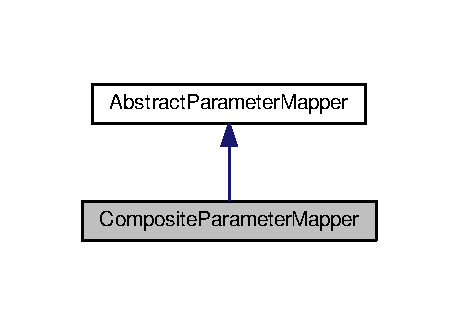
\includegraphics[width=220pt]{classCompositeParameterMapper__inherit__graph}
\end{center}
\end{figure}


Collaboration diagram for Composite\+Parameter\+Mapper\+:\nopagebreak
\begin{figure}[H]
\begin{center}
\leavevmode
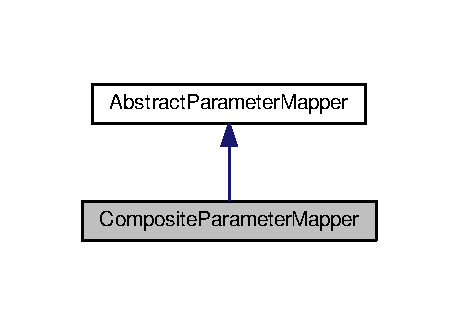
\includegraphics[width=220pt]{classCompositeParameterMapper__coll__graph}
\end{center}
\end{figure}
\subsection*{Public Member Functions}
\begin{DoxyCompactItemize}
\item 
\mbox{\hyperlink{classCompositeParameterMapper_a449747544babe7240562d53944a4742c}{Composite\+Parameter\+Mapper}} (vector$<$ int $>$ \mbox{\hyperlink{classCompositeParameterMapper_ac39d00895ac754c09a81619aba5f644b}{params\+Per\+Mapper}}, vector$<$ \mbox{\hyperlink{classAbstractParameterMapper}{Abstract\+Parameter\+Mapper}} $\ast$$>$ \mbox{\hyperlink{classCompositeParameterMapper_a3f0668fba0502d95363d935ddf9fe9b4}{mappers}})
\item 
virtual \mbox{\hyperlink{classCompositeParameterMapper_a7905cc0fa03c261cb50d8443bb486764}{$\sim$\+Composite\+Parameter\+Mapper}} ()
\item 
vector$<$ double $>$ \mbox{\hyperlink{classCompositeParameterMapper_abac90f20835ad311cfdfc952956b9624}{map}} (vector$<$ double $>$ problem\+Parameters)
\item 
vector$<$ double $>$ \mbox{\hyperlink{classCompositeParameterMapper_a15d15009cf9026b22f27f5d8a5880a4e}{unmap}} (vector$<$ double $>$ kalman\+Parameters)
\end{DoxyCompactItemize}
\subsection*{Private Attributes}
\begin{DoxyCompactItemize}
\item 
vector$<$ \mbox{\hyperlink{classAbstractParameterMapper}{Abstract\+Parameter\+Mapper}} $\ast$ $>$ \mbox{\hyperlink{classCompositeParameterMapper_a3f0668fba0502d95363d935ddf9fe9b4}{mappers}}
\item 
vector$<$ int $>$ \mbox{\hyperlink{classCompositeParameterMapper_ac39d00895ac754c09a81619aba5f644b}{params\+Per\+Mapper}}
\end{DoxyCompactItemize}


\subsection{Detailed Description}
Implementation of the \mbox{\hyperlink{classAbstractParameterMapper}{Abstract\+Parameter\+Mapper}} class using a composite design pattern. It allows to specify a mapper for each parameter (or a subset of parameters). 

Definition at line 21 of file Composite\+Parameter\+Mapper.\+h.



\subsection{Constructor \& Destructor Documentation}
\mbox{\Hypertarget{classCompositeParameterMapper_a449747544babe7240562d53944a4742c}\label{classCompositeParameterMapper_a449747544babe7240562d53944a4742c}} 
\index{Composite\+Parameter\+Mapper@{Composite\+Parameter\+Mapper}!Composite\+Parameter\+Mapper@{Composite\+Parameter\+Mapper}}
\index{Composite\+Parameter\+Mapper@{Composite\+Parameter\+Mapper}!Composite\+Parameter\+Mapper@{Composite\+Parameter\+Mapper}}
\subsubsection{\texorpdfstring{Composite\+Parameter\+Mapper()}{CompositeParameterMapper()}}
{\footnotesize\ttfamily Composite\+Parameter\+Mapper\+::\+Composite\+Parameter\+Mapper (\begin{DoxyParamCaption}\item[{vector$<$ int $>$}]{params\+Per\+Mapper,  }\item[{vector$<$ \mbox{\hyperlink{classAbstractParameterMapper}{Abstract\+Parameter\+Mapper}} $\ast$$>$}]{mappers }\end{DoxyParamCaption})}

Class constructor. 
\begin{DoxyParams}{Parameters}
{\em params\+Per\+Mapper} & Set of the number of parameters treated by each mapper. \\
\hline
{\em mappers} & Set of mapper that map the problem parameters in kalman parameters. \\
\hline
\end{DoxyParams}


Definition at line 11 of file Composite\+Parameter\+Mapper.\+cpp.

\mbox{\Hypertarget{classCompositeParameterMapper_a7905cc0fa03c261cb50d8443bb486764}\label{classCompositeParameterMapper_a7905cc0fa03c261cb50d8443bb486764}} 
\index{Composite\+Parameter\+Mapper@{Composite\+Parameter\+Mapper}!````~Composite\+Parameter\+Mapper@{$\sim$\+Composite\+Parameter\+Mapper}}
\index{````~Composite\+Parameter\+Mapper@{$\sim$\+Composite\+Parameter\+Mapper}!Composite\+Parameter\+Mapper@{Composite\+Parameter\+Mapper}}
\subsubsection{\texorpdfstring{$\sim$\+Composite\+Parameter\+Mapper()}{~CompositeParameterMapper()}}
{\footnotesize\ttfamily Composite\+Parameter\+Mapper\+::$\sim$\+Composite\+Parameter\+Mapper (\begin{DoxyParamCaption}{ }\end{DoxyParamCaption})\hspace{0.3cm}{\ttfamily [virtual]}}

Dummy destructor. 

Definition at line 16 of file Composite\+Parameter\+Mapper.\+cpp.



\subsection{Member Function Documentation}
\mbox{\Hypertarget{classCompositeParameterMapper_abac90f20835ad311cfdfc952956b9624}\label{classCompositeParameterMapper_abac90f20835ad311cfdfc952956b9624}} 
\index{Composite\+Parameter\+Mapper@{Composite\+Parameter\+Mapper}!map@{map}}
\index{map@{map}!Composite\+Parameter\+Mapper@{Composite\+Parameter\+Mapper}}
\subsubsection{\texorpdfstring{map()}{map()}}
{\footnotesize\ttfamily vector$<$ double $>$ Composite\+Parameter\+Mapper\+::map (\begin{DoxyParamCaption}\item[{vector$<$ double $>$}]{problem\+Parameters }\end{DoxyParamCaption})\hspace{0.3cm}{\ttfamily [virtual]}}

Maps the problem parameters into the space of parameters where kalman filter optimize them. 
\begin{DoxyParams}{Parameters}
{\em problem\+Parameters} & Set of problem parameters. \\
\hline
\end{DoxyParams}
\begin{DoxyReturn}{Returns}
Set of kalman parameters 
\end{DoxyReturn}


Implements \mbox{\hyperlink{classAbstractParameterMapper_abb9e78545ff023f2b786b759ec2d23e4}{Abstract\+Parameter\+Mapper}}.



Definition at line 20 of file Composite\+Parameter\+Mapper.\+cpp.

\mbox{\Hypertarget{classCompositeParameterMapper_a15d15009cf9026b22f27f5d8a5880a4e}\label{classCompositeParameterMapper_a15d15009cf9026b22f27f5d8a5880a4e}} 
\index{Composite\+Parameter\+Mapper@{Composite\+Parameter\+Mapper}!unmap@{unmap}}
\index{unmap@{unmap}!Composite\+Parameter\+Mapper@{Composite\+Parameter\+Mapper}}
\subsubsection{\texorpdfstring{unmap()}{unmap()}}
{\footnotesize\ttfamily vector$<$ double $>$ Composite\+Parameter\+Mapper\+::unmap (\begin{DoxyParamCaption}\item[{vector$<$ double $>$}]{kalman\+Parameters }\end{DoxyParamCaption})\hspace{0.3cm}{\ttfamily [virtual]}}

Maps the kalman parameters into the space of problem parameters. 
\begin{DoxyParams}{Parameters}
{\em kalman\+Parameters} & Set of kalman parameters. \\
\hline
\end{DoxyParams}
\begin{DoxyReturn}{Returns}
Set of problem parameters. 
\end{DoxyReturn}


Implements \mbox{\hyperlink{classAbstractParameterMapper_a7fc9715759582e218a3bc38ec43e2d57}{Abstract\+Parameter\+Mapper}}.



Definition at line 33 of file Composite\+Parameter\+Mapper.\+cpp.



\subsection{Member Data Documentation}
\mbox{\Hypertarget{classCompositeParameterMapper_a3f0668fba0502d95363d935ddf9fe9b4}\label{classCompositeParameterMapper_a3f0668fba0502d95363d935ddf9fe9b4}} 
\index{Composite\+Parameter\+Mapper@{Composite\+Parameter\+Mapper}!mappers@{mappers}}
\index{mappers@{mappers}!Composite\+Parameter\+Mapper@{Composite\+Parameter\+Mapper}}
\subsubsection{\texorpdfstring{mappers}{mappers}}
{\footnotesize\ttfamily vector$<$\mbox{\hyperlink{classAbstractParameterMapper}{Abstract\+Parameter\+Mapper}} $\ast$$>$ Composite\+Parameter\+Mapper\+::mappers\hspace{0.3cm}{\ttfamily [private]}}

Set of mapper that map the problem parameters in kalman parameters. 

Definition at line 23 of file Composite\+Parameter\+Mapper.\+h.

\mbox{\Hypertarget{classCompositeParameterMapper_ac39d00895ac754c09a81619aba5f644b}\label{classCompositeParameterMapper_ac39d00895ac754c09a81619aba5f644b}} 
\index{Composite\+Parameter\+Mapper@{Composite\+Parameter\+Mapper}!params\+Per\+Mapper@{params\+Per\+Mapper}}
\index{params\+Per\+Mapper@{params\+Per\+Mapper}!Composite\+Parameter\+Mapper@{Composite\+Parameter\+Mapper}}
\subsubsection{\texorpdfstring{params\+Per\+Mapper}{paramsPerMapper}}
{\footnotesize\ttfamily vector$<$int$>$ Composite\+Parameter\+Mapper\+::params\+Per\+Mapper\hspace{0.3cm}{\ttfamily [private]}}

Set of the number of parameters treated by each mapper. 

Definition at line 25 of file Composite\+Parameter\+Mapper.\+h.



The documentation for this class was generated from the following files\+:\begin{DoxyCompactItemize}
\item 
mapping/Composite\+Parameter\+Mapper.\+h\item 
mapping/Composite\+Parameter\+Mapper.\+cpp\end{DoxyCompactItemize}

\hypertarget{classConfigurationFileReader}{}\section{Configuration\+File\+Reader Class Reference}
\label{classConfigurationFileReader}\index{Configuration\+File\+Reader@{Configuration\+File\+Reader}}


{\ttfamily \#include $<$Configuration\+File\+Reader.\+h$>$}



Collaboration diagram for Configuration\+File\+Reader\+:\nopagebreak
\begin{figure}[H]
\begin{center}
\leavevmode
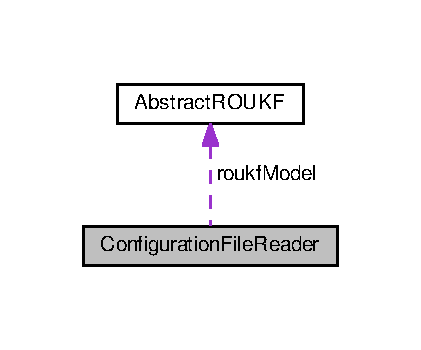
\includegraphics[width=202pt]{classConfigurationFileReader__coll__graph}
\end{center}
\end{figure}
\subsection*{Public Types}
\begin{DoxyCompactItemize}
\item 
enum \mbox{\hyperlink{classConfigurationFileReader_a38105d1480e7e412757a48b9f5d1850a}{F\+I\+L\+T\+E\+R\+\_\+\+T\+Y\+P\+ES}} \{ {\bfseries M\+O\+D\+E\+L\+\_\+\+R\+O\+U\+KF} = 0, 
{\bfseries M\+O\+D\+E\+L\+\_\+\+M\+A\+P\+P\+E\+D\+\_\+\+R\+O\+U\+KF} = 1
 \}
\item 
enum \mbox{\hyperlink{classConfigurationFileReader_adfafe1ca108e6cdb42c3cda28f76628d}{M\+A\+P\+P\+E\+R\+\_\+\+T\+Y\+P\+ES}} \{ {\bfseries I\+D\+E\+N\+T\+I\+TY} = 0, 
{\bfseries E\+X\+P\+O\+N\+E\+N\+T\+I\+AL} = 1, 
{\bfseries S\+I\+G\+M\+O\+I\+D\+AL} = 2
 \}
\end{DoxyCompactItemize}
\subsection*{Public Member Functions}
\begin{DoxyCompactItemize}
\item 
\mbox{\hyperlink{classConfigurationFileReader_ad85a4de7a5b87fcddb1c27de9b3ef332}{Configuration\+File\+Reader}} (string \mbox{\hyperlink{classConfigurationFileReader_a007ec73fe536b697bd200a6b0c66f6e6}{filename}})
\item 
\mbox{\hyperlink{classAbstractROUKF}{Abstract\+R\+O\+U\+KF}} $\ast$ \mbox{\hyperlink{classConfigurationFileReader_a2bea7f730d5caf67b9d3e1bf45072542}{get\+Instance}} ()
\item 
vector$<$ double $>$ \mbox{\hyperlink{classConfigurationFileReader_a1aa7cc335474bd1d15600f93e6de392b}{get\+Observations}} ()
\item 
int \mbox{\hyperlink{classConfigurationFileReader_a3d3b4191df51eb5e560716bc5e034f8a}{get\+N\+Parameters}} () const
\item 
int \mbox{\hyperlink{classConfigurationFileReader_a861fef6643dbc48d92b1eb18305a3931}{get\+N\+States}} () const
\item 
int \mbox{\hyperlink{classConfigurationFileReader_aaf21e598e8fcf28ed762af515946aef1}{get\+N\+Observations}} () const
\end{DoxyCompactItemize}
\subsection*{Private Attributes}
\begin{DoxyCompactItemize}
\item 
string \mbox{\hyperlink{classConfigurationFileReader_a007ec73fe536b697bd200a6b0c66f6e6}{filename}}
\item 
vector$<$ double $>$ \mbox{\hyperlink{classConfigurationFileReader_a556af8eae012e9d7528cbe1fd0e508d0}{observations}}
\item 
int \mbox{\hyperlink{classConfigurationFileReader_ad8cae04fc2c6832bb07446ca87803977}{n\+States}}
\item 
int \mbox{\hyperlink{classConfigurationFileReader_a669b280cc5bc410dba130ee9f14e9cac}{n\+Parameters}}
\item 
int \mbox{\hyperlink{classConfigurationFileReader_a5f6e229fb0ad9c7259a71977c7ead9b3}{n\+Observations}}
\item 
\mbox{\hyperlink{classAbstractROUKF}{Abstract\+R\+O\+U\+KF}} $\ast$ \mbox{\hyperlink{classConfigurationFileReader_a962e727eb22a7ff8d6f4b5a37cbb6a47}{roukf\+Model}}
\end{DoxyCompactItemize}


\subsection{Detailed Description}
File reader class that after parsing the target file generates a Kalman filter instance with appropriate mappers. 

Definition at line 20 of file Configuration\+File\+Reader.\+h.



\subsection{Member Enumeration Documentation}
\mbox{\Hypertarget{classConfigurationFileReader_a38105d1480e7e412757a48b9f5d1850a}\label{classConfigurationFileReader_a38105d1480e7e412757a48b9f5d1850a}} 
\index{Configuration\+File\+Reader@{Configuration\+File\+Reader}!F\+I\+L\+T\+E\+R\+\_\+\+T\+Y\+P\+ES@{F\+I\+L\+T\+E\+R\+\_\+\+T\+Y\+P\+ES}}
\index{F\+I\+L\+T\+E\+R\+\_\+\+T\+Y\+P\+ES@{F\+I\+L\+T\+E\+R\+\_\+\+T\+Y\+P\+ES}!Configuration\+File\+Reader@{Configuration\+File\+Reader}}
\subsubsection{\texorpdfstring{F\+I\+L\+T\+E\+R\+\_\+\+T\+Y\+P\+ES}{FILTER\_TYPES}}
{\footnotesize\ttfamily enum \mbox{\hyperlink{classConfigurationFileReader_a38105d1480e7e412757a48b9f5d1850a}{Configuration\+File\+Reader\+::\+F\+I\+L\+T\+E\+R\+\_\+\+T\+Y\+P\+ES}}}

Types of filter that can be explicit in the configuration file. 

Definition at line 37 of file Configuration\+File\+Reader.\+h.

\mbox{\Hypertarget{classConfigurationFileReader_adfafe1ca108e6cdb42c3cda28f76628d}\label{classConfigurationFileReader_adfafe1ca108e6cdb42c3cda28f76628d}} 
\index{Configuration\+File\+Reader@{Configuration\+File\+Reader}!M\+A\+P\+P\+E\+R\+\_\+\+T\+Y\+P\+ES@{M\+A\+P\+P\+E\+R\+\_\+\+T\+Y\+P\+ES}}
\index{M\+A\+P\+P\+E\+R\+\_\+\+T\+Y\+P\+ES@{M\+A\+P\+P\+E\+R\+\_\+\+T\+Y\+P\+ES}!Configuration\+File\+Reader@{Configuration\+File\+Reader}}
\subsubsection{\texorpdfstring{M\+A\+P\+P\+E\+R\+\_\+\+T\+Y\+P\+ES}{MAPPER\_TYPES}}
{\footnotesize\ttfamily enum \mbox{\hyperlink{classConfigurationFileReader_adfafe1ca108e6cdb42c3cda28f76628d}{Configuration\+File\+Reader\+::\+M\+A\+P\+P\+E\+R\+\_\+\+T\+Y\+P\+ES}}}

Types of mappers that can be explicit in the configuration file. 

Definition at line 39 of file Configuration\+File\+Reader.\+h.



\subsection{Constructor \& Destructor Documentation}
\mbox{\Hypertarget{classConfigurationFileReader_ad85a4de7a5b87fcddb1c27de9b3ef332}\label{classConfigurationFileReader_ad85a4de7a5b87fcddb1c27de9b3ef332}} 
\index{Configuration\+File\+Reader@{Configuration\+File\+Reader}!Configuration\+File\+Reader@{Configuration\+File\+Reader}}
\index{Configuration\+File\+Reader@{Configuration\+File\+Reader}!Configuration\+File\+Reader@{Configuration\+File\+Reader}}
\subsubsection{\texorpdfstring{Configuration\+File\+Reader()}{ConfigurationFileReader()}}
{\footnotesize\ttfamily Configuration\+File\+Reader\+::\+Configuration\+File\+Reader (\begin{DoxyParamCaption}\item[{string}]{filename }\end{DoxyParamCaption})}

Reader constructor. 

Definition at line 24 of file Configuration\+File\+Reader.\+cpp.



\subsection{Member Function Documentation}
\mbox{\Hypertarget{classConfigurationFileReader_a2bea7f730d5caf67b9d3e1bf45072542}\label{classConfigurationFileReader_a2bea7f730d5caf67b9d3e1bf45072542}} 
\index{Configuration\+File\+Reader@{Configuration\+File\+Reader}!get\+Instance@{get\+Instance}}
\index{get\+Instance@{get\+Instance}!Configuration\+File\+Reader@{Configuration\+File\+Reader}}
\subsubsection{\texorpdfstring{get\+Instance()}{getInstance()}}
{\footnotesize\ttfamily \mbox{\hyperlink{classAbstractROUKF}{Abstract\+R\+O\+U\+KF}} $\ast$ Configuration\+File\+Reader\+::get\+Instance (\begin{DoxyParamCaption}{ }\end{DoxyParamCaption})}

Returns the kalman instance associated with the configuration file. \begin{DoxyReturn}{Returns}
Kalman model. 
\end{DoxyReturn}


Definition at line 32 of file Configuration\+File\+Reader.\+cpp.

Here is the call graph for this function\+:\nopagebreak
\begin{figure}[H]
\begin{center}
\leavevmode
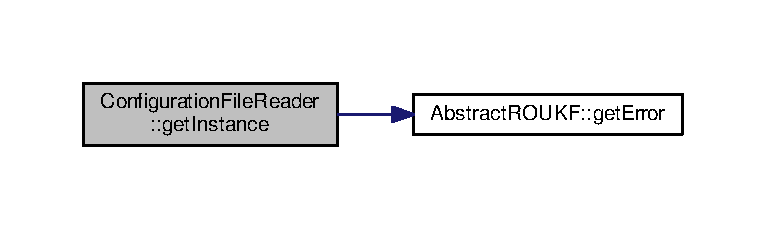
\includegraphics[width=350pt]{classConfigurationFileReader_a2bea7f730d5caf67b9d3e1bf45072542_cgraph}
\end{center}
\end{figure}
\mbox{\Hypertarget{classConfigurationFileReader_aaf21e598e8fcf28ed762af515946aef1}\label{classConfigurationFileReader_aaf21e598e8fcf28ed762af515946aef1}} 
\index{Configuration\+File\+Reader@{Configuration\+File\+Reader}!get\+N\+Observations@{get\+N\+Observations}}
\index{get\+N\+Observations@{get\+N\+Observations}!Configuration\+File\+Reader@{Configuration\+File\+Reader}}
\subsubsection{\texorpdfstring{get\+N\+Observations()}{getNObservations()}}
{\footnotesize\ttfamily int Configuration\+File\+Reader\+::get\+N\+Observations (\begin{DoxyParamCaption}{ }\end{DoxyParamCaption}) const}

Getter for {\ttfamily n\+Observations} \begin{DoxyReturn}{Returns}
{\ttfamily n\+Observations} 
\end{DoxyReturn}


Definition at line 182 of file Configuration\+File\+Reader.\+cpp.

\mbox{\Hypertarget{classConfigurationFileReader_a3d3b4191df51eb5e560716bc5e034f8a}\label{classConfigurationFileReader_a3d3b4191df51eb5e560716bc5e034f8a}} 
\index{Configuration\+File\+Reader@{Configuration\+File\+Reader}!get\+N\+Parameters@{get\+N\+Parameters}}
\index{get\+N\+Parameters@{get\+N\+Parameters}!Configuration\+File\+Reader@{Configuration\+File\+Reader}}
\subsubsection{\texorpdfstring{get\+N\+Parameters()}{getNParameters()}}
{\footnotesize\ttfamily int Configuration\+File\+Reader\+::get\+N\+Parameters (\begin{DoxyParamCaption}{ }\end{DoxyParamCaption}) const}

Getter for {\ttfamily n\+Parameters} \begin{DoxyReturn}{Returns}
{\ttfamily n\+Parameters} 
\end{DoxyReturn}


Definition at line 172 of file Configuration\+File\+Reader.\+cpp.

\mbox{\Hypertarget{classConfigurationFileReader_a861fef6643dbc48d92b1eb18305a3931}\label{classConfigurationFileReader_a861fef6643dbc48d92b1eb18305a3931}} 
\index{Configuration\+File\+Reader@{Configuration\+File\+Reader}!get\+N\+States@{get\+N\+States}}
\index{get\+N\+States@{get\+N\+States}!Configuration\+File\+Reader@{Configuration\+File\+Reader}}
\subsubsection{\texorpdfstring{get\+N\+States()}{getNStates()}}
{\footnotesize\ttfamily int Configuration\+File\+Reader\+::get\+N\+States (\begin{DoxyParamCaption}{ }\end{DoxyParamCaption}) const}

Getter for {\ttfamily n\+States} \begin{DoxyReturn}{Returns}
{\ttfamily n\+States} 
\end{DoxyReturn}


Definition at line 177 of file Configuration\+File\+Reader.\+cpp.

\mbox{\Hypertarget{classConfigurationFileReader_a1aa7cc335474bd1d15600f93e6de392b}\label{classConfigurationFileReader_a1aa7cc335474bd1d15600f93e6de392b}} 
\index{Configuration\+File\+Reader@{Configuration\+File\+Reader}!get\+Observations@{get\+Observations}}
\index{get\+Observations@{get\+Observations}!Configuration\+File\+Reader@{Configuration\+File\+Reader}}
\subsubsection{\texorpdfstring{get\+Observations()}{getObservations()}}
{\footnotesize\ttfamily vector$<$ double $>$ Configuration\+File\+Reader\+::get\+Observations (\begin{DoxyParamCaption}{ }\end{DoxyParamCaption})}

Returns the observations readed from the configuration file after executing get\+Instance. \begin{DoxyReturn}{Returns}
Observations vector. 
\end{DoxyReturn}


Definition at line 168 of file Configuration\+File\+Reader.\+cpp.



\subsection{Member Data Documentation}
\mbox{\Hypertarget{classConfigurationFileReader_a007ec73fe536b697bd200a6b0c66f6e6}\label{classConfigurationFileReader_a007ec73fe536b697bd200a6b0c66f6e6}} 
\index{Configuration\+File\+Reader@{Configuration\+File\+Reader}!filename@{filename}}
\index{filename@{filename}!Configuration\+File\+Reader@{Configuration\+File\+Reader}}
\subsubsection{\texorpdfstring{filename}{filename}}
{\footnotesize\ttfamily string Configuration\+File\+Reader\+::filename\hspace{0.3cm}{\ttfamily [private]}}

Configuration file path. 

Definition at line 22 of file Configuration\+File\+Reader.\+h.

\mbox{\Hypertarget{classConfigurationFileReader_a5f6e229fb0ad9c7259a71977c7ead9b3}\label{classConfigurationFileReader_a5f6e229fb0ad9c7259a71977c7ead9b3}} 
\index{Configuration\+File\+Reader@{Configuration\+File\+Reader}!n\+Observations@{n\+Observations}}
\index{n\+Observations@{n\+Observations}!Configuration\+File\+Reader@{Configuration\+File\+Reader}}
\subsubsection{\texorpdfstring{n\+Observations}{nObservations}}
{\footnotesize\ttfamily int Configuration\+File\+Reader\+::n\+Observations\hspace{0.3cm}{\ttfamily [private]}}

Quantity of observations. 

Definition at line 30 of file Configuration\+File\+Reader.\+h.

\mbox{\Hypertarget{classConfigurationFileReader_a669b280cc5bc410dba130ee9f14e9cac}\label{classConfigurationFileReader_a669b280cc5bc410dba130ee9f14e9cac}} 
\index{Configuration\+File\+Reader@{Configuration\+File\+Reader}!n\+Parameters@{n\+Parameters}}
\index{n\+Parameters@{n\+Parameters}!Configuration\+File\+Reader@{Configuration\+File\+Reader}}
\subsubsection{\texorpdfstring{n\+Parameters}{nParameters}}
{\footnotesize\ttfamily int Configuration\+File\+Reader\+::n\+Parameters\hspace{0.3cm}{\ttfamily [private]}}

Quantity of parameters. 

Definition at line 28 of file Configuration\+File\+Reader.\+h.

\mbox{\Hypertarget{classConfigurationFileReader_ad8cae04fc2c6832bb07446ca87803977}\label{classConfigurationFileReader_ad8cae04fc2c6832bb07446ca87803977}} 
\index{Configuration\+File\+Reader@{Configuration\+File\+Reader}!n\+States@{n\+States}}
\index{n\+States@{n\+States}!Configuration\+File\+Reader@{Configuration\+File\+Reader}}
\subsubsection{\texorpdfstring{n\+States}{nStates}}
{\footnotesize\ttfamily int Configuration\+File\+Reader\+::n\+States\hspace{0.3cm}{\ttfamily [private]}}

Quantity of internal states. 

Definition at line 26 of file Configuration\+File\+Reader.\+h.

\mbox{\Hypertarget{classConfigurationFileReader_a556af8eae012e9d7528cbe1fd0e508d0}\label{classConfigurationFileReader_a556af8eae012e9d7528cbe1fd0e508d0}} 
\index{Configuration\+File\+Reader@{Configuration\+File\+Reader}!observations@{observations}}
\index{observations@{observations}!Configuration\+File\+Reader@{Configuration\+File\+Reader}}
\subsubsection{\texorpdfstring{observations}{observations}}
{\footnotesize\ttfamily vector$<$double$>$ Configuration\+File\+Reader\+::observations\hspace{0.3cm}{\ttfamily [private]}}

Observations loaded from configuration file 

Definition at line 24 of file Configuration\+File\+Reader.\+h.

\mbox{\Hypertarget{classConfigurationFileReader_a962e727eb22a7ff8d6f4b5a37cbb6a47}\label{classConfigurationFileReader_a962e727eb22a7ff8d6f4b5a37cbb6a47}} 
\index{Configuration\+File\+Reader@{Configuration\+File\+Reader}!roukf\+Model@{roukf\+Model}}
\index{roukf\+Model@{roukf\+Model}!Configuration\+File\+Reader@{Configuration\+File\+Reader}}
\subsubsection{\texorpdfstring{roukf\+Model}{roukfModel}}
{\footnotesize\ttfamily \mbox{\hyperlink{classAbstractROUKF}{Abstract\+R\+O\+U\+KF}}$\ast$ Configuration\+File\+Reader\+::roukf\+Model\hspace{0.3cm}{\ttfamily [private]}}

Singleton attribute of the generated kalman filter. 

Definition at line 32 of file Configuration\+File\+Reader.\+h.



The documentation for this class was generated from the following files\+:\begin{DoxyCompactItemize}
\item 
io/Configuration\+File\+Reader.\+h\item 
io/Configuration\+File\+Reader.\+cpp\end{DoxyCompactItemize}

\hypertarget{classExponentialParameterMapper}{}\section{Exponential\+Parameter\+Mapper Class Reference}
\label{classExponentialParameterMapper}\index{Exponential\+Parameter\+Mapper@{Exponential\+Parameter\+Mapper}}


{\ttfamily \#include $<$Exponential\+Parameter\+Mapper.\+h$>$}



Inheritance diagram for Exponential\+Parameter\+Mapper\+:\nopagebreak
\begin{figure}[H]
\begin{center}
\leavevmode
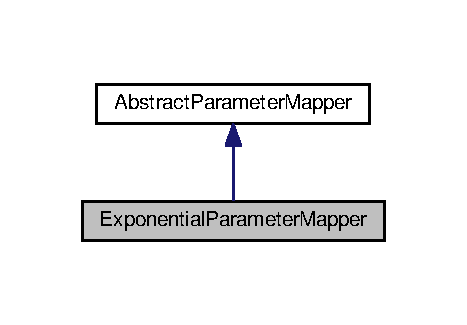
\includegraphics[width=224pt]{classExponentialParameterMapper__inherit__graph}
\end{center}
\end{figure}


Collaboration diagram for Exponential\+Parameter\+Mapper\+:\nopagebreak
\begin{figure}[H]
\begin{center}
\leavevmode
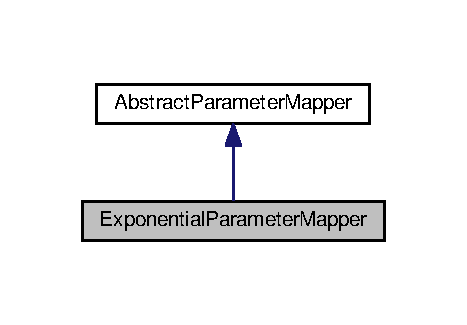
\includegraphics[width=224pt]{classExponentialParameterMapper__coll__graph}
\end{center}
\end{figure}
\subsection*{Public Member Functions}
\begin{DoxyCompactItemize}
\item 
\mbox{\hyperlink{classExponentialParameterMapper_ac2e4af5f64676cb7a3ff664ff92f50fb}{Exponential\+Parameter\+Mapper}} ()
\item 
vector$<$ double $>$ \mbox{\hyperlink{classExponentialParameterMapper_a6abcf5b0efb8ef01ced062b7498c923e}{map}} (vector$<$ double $>$ problem\+Parameters)
\item 
vector$<$ double $>$ \mbox{\hyperlink{classExponentialParameterMapper_ad7040a1ac834e53691bd157df925c545}{unmap}} (vector$<$ double $>$ kalman\+Parameters)
\end{DoxyCompactItemize}


\subsection{Detailed Description}
Implementation of the \mbox{\hyperlink{classAbstractParameterMapper}{Abstract\+Parameter\+Mapper}} class that map the problem parameters into the kalman parameters using a log function. 

Definition at line 17 of file Exponential\+Parameter\+Mapper.\+h.



\subsection{Constructor \& Destructor Documentation}
\mbox{\Hypertarget{classExponentialParameterMapper_ac2e4af5f64676cb7a3ff664ff92f50fb}\label{classExponentialParameterMapper_ac2e4af5f64676cb7a3ff664ff92f50fb}} 
\index{Exponential\+Parameter\+Mapper@{Exponential\+Parameter\+Mapper}!Exponential\+Parameter\+Mapper@{Exponential\+Parameter\+Mapper}}
\index{Exponential\+Parameter\+Mapper@{Exponential\+Parameter\+Mapper}!Exponential\+Parameter\+Mapper@{Exponential\+Parameter\+Mapper}}
\subsubsection{\texorpdfstring{Exponential\+Parameter\+Mapper()}{ExponentialParameterMapper()}}
{\footnotesize\ttfamily Exponential\+Parameter\+Mapper\+::\+Exponential\+Parameter\+Mapper (\begin{DoxyParamCaption}{ }\end{DoxyParamCaption})}

Dummy constructor. 

Definition at line 11 of file Exponential\+Parameter\+Mapper.\+cpp.



\subsection{Member Function Documentation}
\mbox{\Hypertarget{classExponentialParameterMapper_a6abcf5b0efb8ef01ced062b7498c923e}\label{classExponentialParameterMapper_a6abcf5b0efb8ef01ced062b7498c923e}} 
\index{Exponential\+Parameter\+Mapper@{Exponential\+Parameter\+Mapper}!map@{map}}
\index{map@{map}!Exponential\+Parameter\+Mapper@{Exponential\+Parameter\+Mapper}}
\subsubsection{\texorpdfstring{map()}{map()}}
{\footnotesize\ttfamily vector$<$ double $>$ Exponential\+Parameter\+Mapper\+::map (\begin{DoxyParamCaption}\item[{vector$<$ double $>$}]{problem\+Parameters }\end{DoxyParamCaption})\hspace{0.3cm}{\ttfamily [virtual]}}

Maps the problem parameters into the space of parameters where kalman filter optimize them. 
\begin{DoxyParams}{Parameters}
{\em problem\+Parameters} & Set of problem parameters. \\
\hline
\end{DoxyParams}
\begin{DoxyReturn}{Returns}
Set of kalman parameters 
\end{DoxyReturn}


Implements \mbox{\hyperlink{classAbstractParameterMapper_abb9e78545ff023f2b786b759ec2d23e4}{Abstract\+Parameter\+Mapper}}.



Definition at line 14 of file Exponential\+Parameter\+Mapper.\+cpp.

\mbox{\Hypertarget{classExponentialParameterMapper_ad7040a1ac834e53691bd157df925c545}\label{classExponentialParameterMapper_ad7040a1ac834e53691bd157df925c545}} 
\index{Exponential\+Parameter\+Mapper@{Exponential\+Parameter\+Mapper}!unmap@{unmap}}
\index{unmap@{unmap}!Exponential\+Parameter\+Mapper@{Exponential\+Parameter\+Mapper}}
\subsubsection{\texorpdfstring{unmap()}{unmap()}}
{\footnotesize\ttfamily vector$<$ double $>$ Exponential\+Parameter\+Mapper\+::unmap (\begin{DoxyParamCaption}\item[{vector$<$ double $>$}]{kalman\+Parameters }\end{DoxyParamCaption})\hspace{0.3cm}{\ttfamily [virtual]}}

Maps the kalman parameters into the space of problem parameters. 
\begin{DoxyParams}{Parameters}
{\em kalman\+Parameters} & Set of kalman parameters. \\
\hline
\end{DoxyParams}
\begin{DoxyReturn}{Returns}
Set of problem parameters. 
\end{DoxyReturn}


Implements \mbox{\hyperlink{classAbstractParameterMapper_a7fc9715759582e218a3bc38ec43e2d57}{Abstract\+Parameter\+Mapper}}.



Definition at line 23 of file Exponential\+Parameter\+Mapper.\+cpp.



The documentation for this class was generated from the following files\+:\begin{DoxyCompactItemize}
\item 
mapping/Exponential\+Parameter\+Mapper.\+h\item 
mapping/Exponential\+Parameter\+Mapper.\+cpp\end{DoxyCompactItemize}

\hypertarget{classIdentityParameterMapper}{}\section{Identity\+Parameter\+Mapper Class Reference}
\label{classIdentityParameterMapper}\index{Identity\+Parameter\+Mapper@{Identity\+Parameter\+Mapper}}


{\ttfamily \#include $<$Identity\+Parameter\+Mapper.\+h$>$}



Inheritance diagram for Identity\+Parameter\+Mapper\+:\nopagebreak
\begin{figure}[H]
\begin{center}
\leavevmode
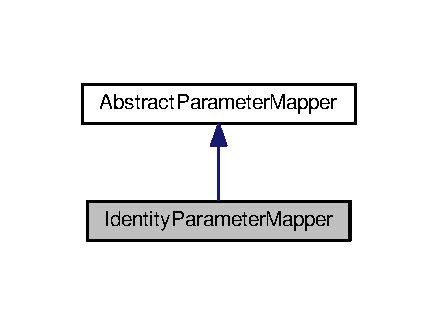
\includegraphics[width=210pt]{classIdentityParameterMapper__inherit__graph}
\end{center}
\end{figure}


Collaboration diagram for Identity\+Parameter\+Mapper\+:\nopagebreak
\begin{figure}[H]
\begin{center}
\leavevmode
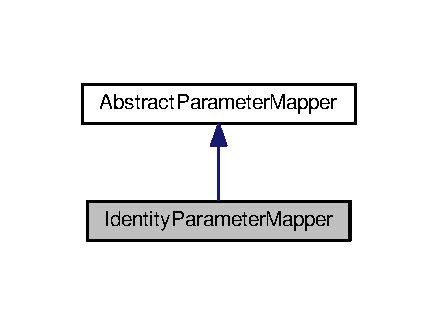
\includegraphics[width=210pt]{classIdentityParameterMapper__coll__graph}
\end{center}
\end{figure}
\subsection*{Public Member Functions}
\begin{DoxyCompactItemize}
\item 
\mbox{\hyperlink{classIdentityParameterMapper_ae09bce8a0343460df2dc251fede4b8ce}{Identity\+Parameter\+Mapper}} ()
\item 
vector$<$ double $>$ \mbox{\hyperlink{classIdentityParameterMapper_a21105fcfd2e89ac5529f97433f03b1c3}{map}} (vector$<$ double $>$ problem\+Parameters)
\item 
vector$<$ double $>$ \mbox{\hyperlink{classIdentityParameterMapper_ad7ad11e683701104024a553eb8f2373b}{unmap}} (vector$<$ double $>$ kalman\+Parameters)
\end{DoxyCompactItemize}


\subsection{Detailed Description}
Implementation of the \mbox{\hyperlink{classAbstractParameterMapper}{Abstract\+Parameter\+Mapper}} class that maps the problem parameters directly in the kalman parameter space without modifications. 

Definition at line 17 of file Identity\+Parameter\+Mapper.\+h.



\subsection{Constructor \& Destructor Documentation}
\mbox{\Hypertarget{classIdentityParameterMapper_ae09bce8a0343460df2dc251fede4b8ce}\label{classIdentityParameterMapper_ae09bce8a0343460df2dc251fede4b8ce}} 
\index{Identity\+Parameter\+Mapper@{Identity\+Parameter\+Mapper}!Identity\+Parameter\+Mapper@{Identity\+Parameter\+Mapper}}
\index{Identity\+Parameter\+Mapper@{Identity\+Parameter\+Mapper}!Identity\+Parameter\+Mapper@{Identity\+Parameter\+Mapper}}
\subsubsection{\texorpdfstring{Identity\+Parameter\+Mapper()}{IdentityParameterMapper()}}
{\footnotesize\ttfamily Identity\+Parameter\+Mapper\+::\+Identity\+Parameter\+Mapper (\begin{DoxyParamCaption}{ }\end{DoxyParamCaption})}

Dummy constructor. 

Definition at line 10 of file Identity\+Parameter\+Mapper.\+cpp.



\subsection{Member Function Documentation}
\mbox{\Hypertarget{classIdentityParameterMapper_a21105fcfd2e89ac5529f97433f03b1c3}\label{classIdentityParameterMapper_a21105fcfd2e89ac5529f97433f03b1c3}} 
\index{Identity\+Parameter\+Mapper@{Identity\+Parameter\+Mapper}!map@{map}}
\index{map@{map}!Identity\+Parameter\+Mapper@{Identity\+Parameter\+Mapper}}
\subsubsection{\texorpdfstring{map()}{map()}}
{\footnotesize\ttfamily vector$<$ double $>$ Identity\+Parameter\+Mapper\+::map (\begin{DoxyParamCaption}\item[{vector$<$ double $>$}]{problem\+Parameters }\end{DoxyParamCaption})\hspace{0.3cm}{\ttfamily [virtual]}}

Maps the problem parameters into the space of parameters where kalman filter optimize them. 
\begin{DoxyParams}{Parameters}
{\em problem\+Parameters} & Set of problem parameters. \\
\hline
\end{DoxyParams}
\begin{DoxyReturn}{Returns}
Set of kalman parameters 
\end{DoxyReturn}


Implements \mbox{\hyperlink{classAbstractParameterMapper_abb9e78545ff023f2b786b759ec2d23e4}{Abstract\+Parameter\+Mapper}}.



Definition at line 13 of file Identity\+Parameter\+Mapper.\+cpp.

\mbox{\Hypertarget{classIdentityParameterMapper_ad7ad11e683701104024a553eb8f2373b}\label{classIdentityParameterMapper_ad7ad11e683701104024a553eb8f2373b}} 
\index{Identity\+Parameter\+Mapper@{Identity\+Parameter\+Mapper}!unmap@{unmap}}
\index{unmap@{unmap}!Identity\+Parameter\+Mapper@{Identity\+Parameter\+Mapper}}
\subsubsection{\texorpdfstring{unmap()}{unmap()}}
{\footnotesize\ttfamily vector$<$ double $>$ Identity\+Parameter\+Mapper\+::unmap (\begin{DoxyParamCaption}\item[{vector$<$ double $>$}]{kalman\+Parameters }\end{DoxyParamCaption})\hspace{0.3cm}{\ttfamily [virtual]}}

Maps the kalman parameters into the space of problem parameters. 
\begin{DoxyParams}{Parameters}
{\em kalman\+Parameters} & Set of kalman parameters. \\
\hline
\end{DoxyParams}
\begin{DoxyReturn}{Returns}
Set of problem parameters. 
\end{DoxyReturn}


Implements \mbox{\hyperlink{classAbstractParameterMapper_a7fc9715759582e218a3bc38ec43e2d57}{Abstract\+Parameter\+Mapper}}.



Definition at line 17 of file Identity\+Parameter\+Mapper.\+cpp.



The documentation for this class was generated from the following files\+:\begin{DoxyCompactItemize}
\item 
mapping/Identity\+Parameter\+Mapper.\+h\item 
mapping/Identity\+Parameter\+Mapper.\+cpp\end{DoxyCompactItemize}

\hypertarget{classMappedROUKF}{}\section{Mapped\+R\+O\+U\+KF Class Reference}
\label{classMappedROUKF}\index{Mapped\+R\+O\+U\+KF@{Mapped\+R\+O\+U\+KF}}


{\ttfamily \#include $<$Mapped\+R\+O\+U\+K\+F.\+h$>$}



Inheritance diagram for Mapped\+R\+O\+U\+KF\+:\nopagebreak
\begin{figure}[H]
\begin{center}
\leavevmode
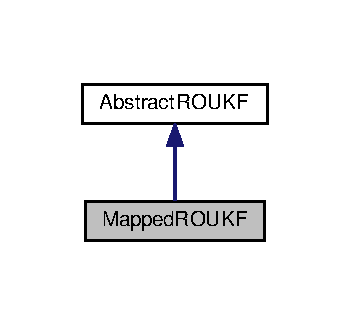
\includegraphics[width=168pt]{classMappedROUKF__inherit__graph}
\end{center}
\end{figure}


Collaboration diagram for Mapped\+R\+O\+U\+KF\+:\nopagebreak
\begin{figure}[H]
\begin{center}
\leavevmode
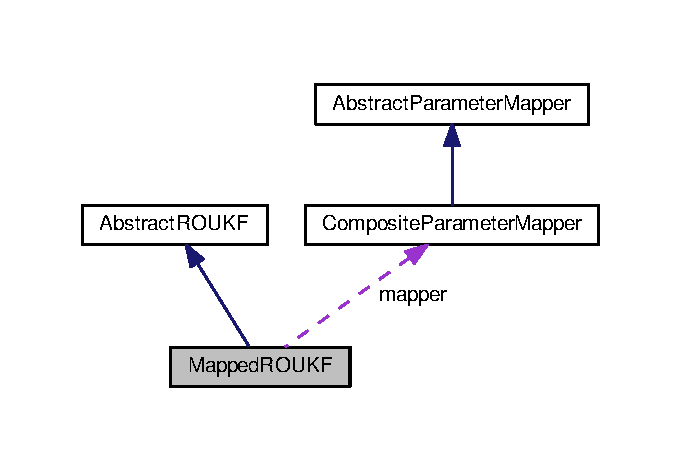
\includegraphics[width=327pt]{classMappedROUKF__coll__graph}
\end{center}
\end{figure}
\subsection*{Public Types}
\begin{DoxyCompactItemize}
\item 
enum \mbox{\hyperlink{classMappedROUKF_a9aa29956ea12176771fbec185601deca}{M\+A\+P\+P\+I\+N\+G\+\_\+\+T\+Y\+PE}} \{ {\bfseries D\+E\+F\+A\+U\+LT}, 
{\bfseries P\+O\+S\+I\+T\+I\+VE}, 
{\bfseries R\+A\+N\+G\+ED}
 \}
\end{DoxyCompactItemize}
\subsection*{Public Member Functions}
\begin{DoxyCompactItemize}
\item 
\mbox{\hyperlink{classMappedROUKF_a3747b98efef856486df6428746807808}{Mapped\+R\+O\+U\+KF}} (int \mbox{\hyperlink{classAbstractROUKF_a4f6403f7fd2fac691e4ac516f47c0a06}{n\+Observations}}, int \mbox{\hyperlink{classAbstractROUKF_af9ce480feb5d97761f20fdd546878aff}{n\+States}}, int \mbox{\hyperlink{classAbstractROUKF_a488f708dcdd66758cd879421cd454846}{n\+Parameters}}, vector$<$ double $>$ observations\+Uncertainty, vector$<$ double $>$ parameters\+Uncertainty, \mbox{\hyperlink{classSigmaPointsGenerator_ad6f9474c0313425a10add120e0acf944}{Sigma\+Points\+Generator\+::\+S\+I\+G\+M\+A\+\_\+\+D\+I\+S\+T\+R\+I\+B\+U\+T\+I\+ON}} sigma\+Distribution)
\item 
\mbox{\hyperlink{classMappedROUKF_a0febaff07fa4b563653ed83ab9f3a753}{Mapped\+R\+O\+U\+KF}} (int \mbox{\hyperlink{classAbstractROUKF_a4f6403f7fd2fac691e4ac516f47c0a06}{n\+Observations}}, int \mbox{\hyperlink{classAbstractROUKF_af9ce480feb5d97761f20fdd546878aff}{n\+States}}, int \mbox{\hyperlink{classAbstractROUKF_a488f708dcdd66758cd879421cd454846}{n\+Parameters}}, vector$<$ double $>$ observations\+Uncertainty, vector$<$ double $>$ parameters\+Uncertainty, \mbox{\hyperlink{classSigmaPointsGenerator_ad6f9474c0313425a10add120e0acf944}{Sigma\+Points\+Generator\+::\+S\+I\+G\+M\+A\+\_\+\+D\+I\+S\+T\+R\+I\+B\+U\+T\+I\+ON}} sigma\+Distribution, \mbox{\hyperlink{classMappedROUKF_a9aa29956ea12176771fbec185601deca}{Mapped\+R\+O\+U\+K\+F\+::\+M\+A\+P\+P\+I\+N\+G\+\_\+\+T\+Y\+PE}} mapping\+Type, vector$<$ double $>$ mapping\+Parameters)
\item 
\mbox{\hyperlink{classMappedROUKF_a37d0e3963e90076ce32f41189e088ed0}{Mapped\+R\+O\+U\+KF}} (int \mbox{\hyperlink{classAbstractROUKF_a4f6403f7fd2fac691e4ac516f47c0a06}{n\+Observations}}, int \mbox{\hyperlink{classAbstractROUKF_af9ce480feb5d97761f20fdd546878aff}{n\+States}}, int \mbox{\hyperlink{classAbstractROUKF_a488f708dcdd66758cd879421cd454846}{n\+Parameters}}, vector$<$ double $>$ observations\+Uncertainty, vector$<$ double $>$ parameters\+Uncertainty, \mbox{\hyperlink{classSigmaPointsGenerator_ad6f9474c0313425a10add120e0acf944}{Sigma\+Points\+Generator\+::\+S\+I\+G\+M\+A\+\_\+\+D\+I\+S\+T\+R\+I\+B\+U\+T\+I\+ON}} sigma\+Distribution, \mbox{\hyperlink{classCompositeParameterMapper}{Composite\+Parameter\+Mapper}} $\ast$\mbox{\hyperlink{classMappedROUKF_a5177d0749fa9a6ce81d760267f4e7e09}{mapper}})
\item 
\mbox{\hyperlink{classMappedROUKF_a62754db5475cbfc001f2dc298a2092d0}{$\sim$\+Mapped\+R\+O\+U\+KF}} ()
\item 
double \mbox{\hyperlink{classMappedROUKF_a0a91ee2acdfa66f4f788ebcc920e112a}{execute\+Step}} (vector$<$ double $>$ Zkhatc, forward\+Op A, observation\+Op H)
\item 
double \mbox{\hyperlink{classMappedROUKF_ab6a3f488ef97ee3d8e11efa5aa0385c7}{execute\+Step\+Parallel}} (vector$<$ double $>$ Zkhatc, forward\+Op A, observation\+Op H, int seed, M\+P\+I\+\_\+\+Comm local\+\_\+comm, M\+P\+I\+\_\+\+Comm masters\+\_\+comm)
\item 
void \mbox{\hyperlink{classMappedROUKF_ad4ddf881c1ade83fe0cc2ab99ad58b7e}{reset}} (int \mbox{\hyperlink{classAbstractROUKF_a4f6403f7fd2fac691e4ac516f47c0a06}{n\+Observations}}, int \mbox{\hyperlink{classAbstractROUKF_af9ce480feb5d97761f20fdd546878aff}{n\+States}}, int \mbox{\hyperlink{classAbstractROUKF_a488f708dcdd66758cd879421cd454846}{n\+Parameters}}, vector$<$ double $>$ observations\+Uncertainty, vector$<$ double $>$ parameters\+Uncertainty, \mbox{\hyperlink{classSigmaPointsGenerator_ad6f9474c0313425a10add120e0acf944}{Sigma\+Points\+Generator\+::\+S\+I\+G\+M\+A\+\_\+\+D\+I\+S\+T\+R\+I\+B\+U\+T\+I\+ON}} sigma\+Distribution)
\item 
void \mbox{\hyperlink{classMappedROUKF_ad84ef097844217e5c5342e2ee8968521}{replace\+Mapper}} (\mbox{\hyperlink{classCompositeParameterMapper}{Composite\+Parameter\+Mapper}} $\ast$\mbox{\hyperlink{classMappedROUKF_a5177d0749fa9a6ce81d760267f4e7e09}{mapper}})
\item 
virtual void \mbox{\hyperlink{classMappedROUKF_aa6670e2cc9899b93b71db3f238ae93f3}{get\+Parameters}} (double $\ast$$\ast$ThetaC) override
\item 
virtual void \mbox{\hyperlink{classMappedROUKF_a4d3a109dc95812c8d9c6ac2a489349c2}{set\+Parameters}} (double $\ast$ThetaC) override
\end{DoxyCompactItemize}
\subsection*{Private Attributes}
\begin{DoxyCompactItemize}
\item 
\mbox{\hyperlink{classCompositeParameterMapper}{Composite\+Parameter\+Mapper}} $\ast$ \mbox{\hyperlink{classMappedROUKF_a5177d0749fa9a6ce81d760267f4e7e09}{mapper}}
\end{DoxyCompactItemize}
\subsection*{Additional Inherited Members}


\subsection{Detailed Description}
An example for the usage of the library\+:


\begin{DoxyCode}
   int (*ptA)(\textcolor{keywordtype}{double}*, int) = NULL;
void (*ptH)(\textcolor{keywordtype}{double}*, int, \textcolor{keywordtype}{double}*, int) = NULL;
ptA = \&forwardOpElasticity;
ptH = \&observerOpElasticity;

 \textcolor{comment}{//    Initialization parameters}
\textcolor{keywordflow}{for} (\textcolor{keywordtype}{int} i = 0; i < \mbox{\hyperlink{classAbstractROUKF_a488f708dcdd66758cd879421cd454846}{nParameters}}; i++) \{
   initialGuess[i] = 2.5E5;            \textcolor{comment}{// -> X0}
   parametersUncertainties[i] =1E8;    \textcolor{comment}{// -> U0^\{-1\}}
\}
\mbox{\hyperlink{classROUKF}{ROUKF}} *kalmanInstance = \textcolor{keyword}{new} \mbox{\hyperlink{classROUKF}{ROUKF}}(\mbox{\hyperlink{classAbstractROUKF_af9ce480feb5d97761f20fdd546878aff}{nStates}}, \mbox{\hyperlink{classAbstractROUKF_a488f708dcdd66758cd879421cd454846}{nParameters}}, statesUncertainties,
parametersUncertainties);

\textcolor{comment}{// Set initial condition}
kalmanInstance->\mbox{\hyperlink{classAbstractROUKF_a618f4719892c0997e5f62cc23913aa12}{setState}}(initialGuess, \mbox{\hyperlink{classAbstractROUKF_a488f708dcdd66758cd879421cd454846}{nParameters}});

\textcolor{keywordflow}{for} (\textcolor{keywordtype}{int} it = 0; it < 3000; it++) \{
   \mbox{\hyperlink{classAbstractROUKF_a551d0b61b010efe7923358c93cbd0db5}{error}} = kalmanInstance->\mbox{\hyperlink{classROUKF_ad200c0176a1e6e443fbea55bd8905dd6}{executeStep}}(observation, \mbox{\hyperlink{classAbstractROUKF_af9ce480feb5d97761f20fdd546878aff}{nStates}}, ptA, ptH);
\}

\textcolor{comment}{// Get the Kalman estimation}
kalmanInstance->\mbox{\hyperlink{classAbstractROUKF_ad24dafa1f4cb02a38958264740588b87}{getState}}(\&sol);            \textcolor{comment}{// -> XSol}
\end{DoxyCode}
 Class that implements the reduced order unscented Kalman filter. 

Definition at line 57 of file Mapped\+R\+O\+U\+K\+F.\+h.



\subsection{Member Enumeration Documentation}
\mbox{\Hypertarget{classMappedROUKF_a9aa29956ea12176771fbec185601deca}\label{classMappedROUKF_a9aa29956ea12176771fbec185601deca}} 
\index{Mapped\+R\+O\+U\+KF@{Mapped\+R\+O\+U\+KF}!M\+A\+P\+P\+I\+N\+G\+\_\+\+T\+Y\+PE@{M\+A\+P\+P\+I\+N\+G\+\_\+\+T\+Y\+PE}}
\index{M\+A\+P\+P\+I\+N\+G\+\_\+\+T\+Y\+PE@{M\+A\+P\+P\+I\+N\+G\+\_\+\+T\+Y\+PE}!Mapped\+R\+O\+U\+KF@{Mapped\+R\+O\+U\+KF}}
\subsubsection{\texorpdfstring{M\+A\+P\+P\+I\+N\+G\+\_\+\+T\+Y\+PE}{MAPPING\_TYPE}}
{\footnotesize\ttfamily enum \mbox{\hyperlink{classMappedROUKF_a9aa29956ea12176771fbec185601deca}{Mapped\+R\+O\+U\+K\+F\+::\+M\+A\+P\+P\+I\+N\+G\+\_\+\+T\+Y\+PE}}}

Reparametrization type. 

Definition at line 64 of file Mapped\+R\+O\+U\+K\+F.\+h.



\subsection{Constructor \& Destructor Documentation}
\mbox{\Hypertarget{classMappedROUKF_a3747b98efef856486df6428746807808}\label{classMappedROUKF_a3747b98efef856486df6428746807808}} 
\index{Mapped\+R\+O\+U\+KF@{Mapped\+R\+O\+U\+KF}!Mapped\+R\+O\+U\+KF@{Mapped\+R\+O\+U\+KF}}
\index{Mapped\+R\+O\+U\+KF@{Mapped\+R\+O\+U\+KF}!Mapped\+R\+O\+U\+KF@{Mapped\+R\+O\+U\+KF}}
\subsubsection{\texorpdfstring{Mapped\+R\+O\+U\+K\+F()}{MappedROUKF()}\hspace{0.1cm}{\footnotesize\ttfamily [1/3]}}
{\footnotesize\ttfamily Mapped\+R\+O\+U\+K\+F\+::\+Mapped\+R\+O\+U\+KF (\begin{DoxyParamCaption}\item[{int}]{n\+Observations,  }\item[{int}]{n\+States,  }\item[{int}]{n\+Parameters,  }\item[{vector$<$ double $>$}]{observations\+Uncertainty,  }\item[{vector$<$ double $>$}]{parameters\+Uncertainty,  }\item[{\mbox{\hyperlink{classSigmaPointsGenerator_ad6f9474c0313425a10add120e0acf944}{Sigma\+Points\+Generator\+::\+S\+I\+G\+M\+A\+\_\+\+D\+I\+S\+T\+R\+I\+B\+U\+T\+I\+ON}}}]{sigma\+Distribution }\end{DoxyParamCaption})}

Creates the covariance matrixes and sigma points associated with the extended vector X and their uncertainty. 
\begin{DoxyParams}{Parameters}
{\em n\+Observations} & Quantity of observations. \\
\hline
{\em n\+States} & Quantity of states. \\
\hline
{\em n\+Parameters} & Quantity of parameters. \\
\hline
{\em observations\+Uncertainty} & Vector with the uncertainty of each state in X. \\
\hline
{\em parameters\+Uncertainty} & Vector with the uncertainty of each parameter in Theta. \\
\hline
{\em sigma\+Distribution} & Type of sigmas applied to assess the unscented transform. \\
\hline
\end{DoxyParams}


Definition at line 18 of file Mapped\+R\+O\+U\+K\+F.\+cpp.

Here is the call graph for this function\+:\nopagebreak
\begin{figure}[H]
\begin{center}
\leavevmode
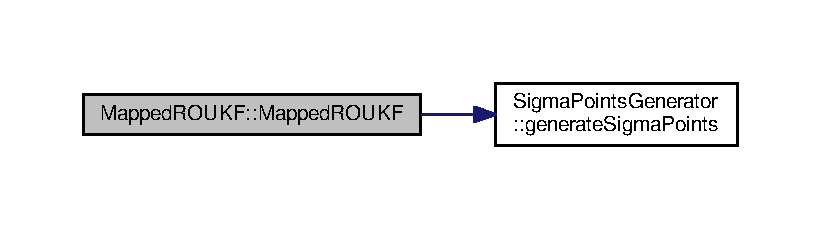
\includegraphics[width=350pt]{classMappedROUKF_a3747b98efef856486df6428746807808_cgraph}
\end{center}
\end{figure}
\mbox{\Hypertarget{classMappedROUKF_a0febaff07fa4b563653ed83ab9f3a753}\label{classMappedROUKF_a0febaff07fa4b563653ed83ab9f3a753}} 
\index{Mapped\+R\+O\+U\+KF@{Mapped\+R\+O\+U\+KF}!Mapped\+R\+O\+U\+KF@{Mapped\+R\+O\+U\+KF}}
\index{Mapped\+R\+O\+U\+KF@{Mapped\+R\+O\+U\+KF}!Mapped\+R\+O\+U\+KF@{Mapped\+R\+O\+U\+KF}}
\subsubsection{\texorpdfstring{Mapped\+R\+O\+U\+K\+F()}{MappedROUKF()}\hspace{0.1cm}{\footnotesize\ttfamily [2/3]}}
{\footnotesize\ttfamily Mapped\+R\+O\+U\+K\+F\+::\+Mapped\+R\+O\+U\+KF (\begin{DoxyParamCaption}\item[{int}]{n\+Observations,  }\item[{int}]{n\+States,  }\item[{int}]{n\+Parameters,  }\item[{vector$<$ double $>$}]{observations\+Uncertainty,  }\item[{vector$<$ double $>$}]{parameters\+Uncertainty,  }\item[{\mbox{\hyperlink{classSigmaPointsGenerator_ad6f9474c0313425a10add120e0acf944}{Sigma\+Points\+Generator\+::\+S\+I\+G\+M\+A\+\_\+\+D\+I\+S\+T\+R\+I\+B\+U\+T\+I\+ON}}}]{sigma\+Distribution,  }\item[{\mbox{\hyperlink{classMappedROUKF_a9aa29956ea12176771fbec185601deca}{Mapped\+R\+O\+U\+K\+F\+::\+M\+A\+P\+P\+I\+N\+G\+\_\+\+T\+Y\+PE}}}]{mapping\+Type,  }\item[{vector$<$ double $>$}]{mapping\+Parameters }\end{DoxyParamCaption})}

Creates the covariance matrixes and sigma points associated with the extended vector X and their uncertainty. The chosen mapping is the same for all parameters. 
\begin{DoxyParams}{Parameters}
{\em n\+Observations} & Quantity of observations. \\
\hline
{\em n\+States} & Quantity of states. \\
\hline
{\em n\+Parameters} & Quantity of parameters. \\
\hline
{\em observations\+Uncertainty} & Vector with the uncertainty of each state in X. \\
\hline
{\em parameters\+Uncertainty} & Vector with the uncertainty of each parameter in Theta. \\
\hline
{\em sigma\+Distribution} & Type of sigmas applied to assess the unscented transform. \\
\hline
{\em mapping\+Type} & Type of mapping between the problem and the kalman parameters. \\
\hline
{\em mapping\+Parameters} & Parameters for the chosen mapping type. \\
\hline
\end{DoxyParams}


Definition at line 52 of file Mapped\+R\+O\+U\+K\+F.\+cpp.

Here is the call graph for this function\+:\nopagebreak
\begin{figure}[H]
\begin{center}
\leavevmode
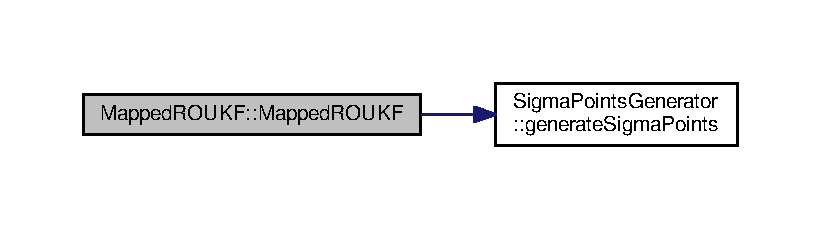
\includegraphics[width=350pt]{classMappedROUKF_a0febaff07fa4b563653ed83ab9f3a753_cgraph}
\end{center}
\end{figure}
\mbox{\Hypertarget{classMappedROUKF_a37d0e3963e90076ce32f41189e088ed0}\label{classMappedROUKF_a37d0e3963e90076ce32f41189e088ed0}} 
\index{Mapped\+R\+O\+U\+KF@{Mapped\+R\+O\+U\+KF}!Mapped\+R\+O\+U\+KF@{Mapped\+R\+O\+U\+KF}}
\index{Mapped\+R\+O\+U\+KF@{Mapped\+R\+O\+U\+KF}!Mapped\+R\+O\+U\+KF@{Mapped\+R\+O\+U\+KF}}
\subsubsection{\texorpdfstring{Mapped\+R\+O\+U\+K\+F()}{MappedROUKF()}\hspace{0.1cm}{\footnotesize\ttfamily [3/3]}}
{\footnotesize\ttfamily Mapped\+R\+O\+U\+K\+F\+::\+Mapped\+R\+O\+U\+KF (\begin{DoxyParamCaption}\item[{int}]{n\+Observations,  }\item[{int}]{n\+States,  }\item[{int}]{n\+Parameters,  }\item[{vector$<$ double $>$}]{observations\+Uncertainty,  }\item[{vector$<$ double $>$}]{parameters\+Uncertainty,  }\item[{\mbox{\hyperlink{classSigmaPointsGenerator_ad6f9474c0313425a10add120e0acf944}{Sigma\+Points\+Generator\+::\+S\+I\+G\+M\+A\+\_\+\+D\+I\+S\+T\+R\+I\+B\+U\+T\+I\+ON}}}]{sigma\+Distribution,  }\item[{\mbox{\hyperlink{classCompositeParameterMapper}{Composite\+Parameter\+Mapper}} $\ast$}]{mapper }\end{DoxyParamCaption})}

Creates the covariance matrixes and sigma points associated with the extended vector X and their uncertainty. The mapping between the problem and the kalman parameters is given by the user customized {\ttfamily mapper} mapping function. 
\begin{DoxyParams}{Parameters}
{\em n\+Observations} & Quantity of observations. \\
\hline
{\em n\+States} & Quantity of states. \\
\hline
{\em n\+Parameters} & Quantity of parameters. \\
\hline
{\em observations\+Uncertainty} & Vector with the uncertainty of each state in X. \\
\hline
{\em parameters\+Uncertainty} & Vector with the uncertainty of each parameter in Theta. \\
\hline
{\em sigma\+Distribution} & Type of sigmas applied to assess the unscented transform. \\
\hline
{\em mapper} & User customized mapping function between the problem and the kalman parameters. \\
\hline
\end{DoxyParams}


Definition at line 99 of file Mapped\+R\+O\+U\+K\+F.\+cpp.

Here is the call graph for this function\+:\nopagebreak
\begin{figure}[H]
\begin{center}
\leavevmode
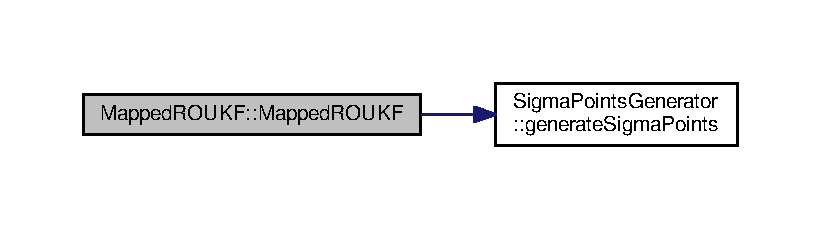
\includegraphics[width=350pt]{classMappedROUKF_a37d0e3963e90076ce32f41189e088ed0_cgraph}
\end{center}
\end{figure}
\mbox{\Hypertarget{classMappedROUKF_a62754db5475cbfc001f2dc298a2092d0}\label{classMappedROUKF_a62754db5475cbfc001f2dc298a2092d0}} 
\index{Mapped\+R\+O\+U\+KF@{Mapped\+R\+O\+U\+KF}!````~Mapped\+R\+O\+U\+KF@{$\sim$\+Mapped\+R\+O\+U\+KF}}
\index{````~Mapped\+R\+O\+U\+KF@{$\sim$\+Mapped\+R\+O\+U\+KF}!Mapped\+R\+O\+U\+KF@{Mapped\+R\+O\+U\+KF}}
\subsubsection{\texorpdfstring{$\sim$\+Mapped\+R\+O\+U\+K\+F()}{~MappedROUKF()}}
{\footnotesize\ttfamily Mapped\+R\+O\+U\+K\+F\+::$\sim$\+Mapped\+R\+O\+U\+KF (\begin{DoxyParamCaption}{ }\end{DoxyParamCaption})}

Void destructor. 

Definition at line 129 of file Mapped\+R\+O\+U\+K\+F.\+cpp.



\subsection{Member Function Documentation}
\mbox{\Hypertarget{classMappedROUKF_a0a91ee2acdfa66f4f788ebcc920e112a}\label{classMappedROUKF_a0a91ee2acdfa66f4f788ebcc920e112a}} 
\index{Mapped\+R\+O\+U\+KF@{Mapped\+R\+O\+U\+KF}!execute\+Step@{execute\+Step}}
\index{execute\+Step@{execute\+Step}!Mapped\+R\+O\+U\+KF@{Mapped\+R\+O\+U\+KF}}
\subsubsection{\texorpdfstring{execute\+Step()}{executeStep()}}
{\footnotesize\ttfamily double Mapped\+R\+O\+U\+K\+F\+::execute\+Step (\begin{DoxyParamCaption}\item[{vector$<$ double $>$}]{Zkhatc,  }\item[{forward\+Op}]{A,  }\item[{observation\+Op}]{H }\end{DoxyParamCaption})}

Performs one step of the Kalman filtering process in serial execution of the sigma points. 
\begin{DoxyParams}{Parameters}
{\em Zkhatc} & Current observations estimations. \\
\hline
{\em A} & Forward operator. \\
\hline
{\em H} & Observation operator; \\
\hline
\end{DoxyParams}
\begin{DoxyReturn}{Returns}
Current L2 norm of the errors across all observations. 
\end{DoxyReturn}


Definition at line 132 of file Mapped\+R\+O\+U\+K\+F.\+cpp.

Here is the call graph for this function\+:\nopagebreak
\begin{figure}[H]
\begin{center}
\leavevmode
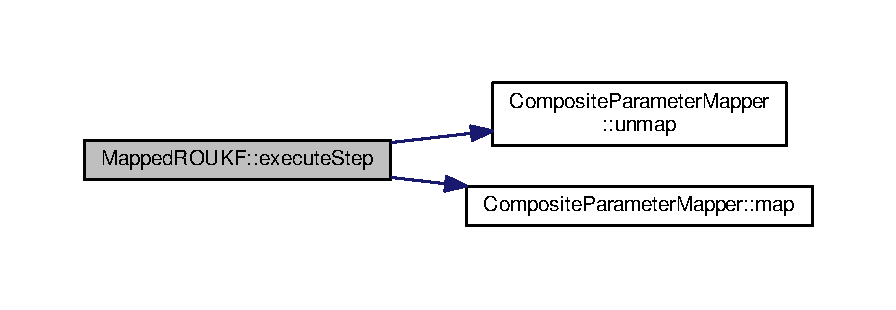
\includegraphics[width=350pt]{classMappedROUKF_a0a91ee2acdfa66f4f788ebcc920e112a_cgraph}
\end{center}
\end{figure}
\mbox{\Hypertarget{classMappedROUKF_ab6a3f488ef97ee3d8e11efa5aa0385c7}\label{classMappedROUKF_ab6a3f488ef97ee3d8e11efa5aa0385c7}} 
\index{Mapped\+R\+O\+U\+KF@{Mapped\+R\+O\+U\+KF}!execute\+Step\+Parallel@{execute\+Step\+Parallel}}
\index{execute\+Step\+Parallel@{execute\+Step\+Parallel}!Mapped\+R\+O\+U\+KF@{Mapped\+R\+O\+U\+KF}}
\subsubsection{\texorpdfstring{execute\+Step\+Parallel()}{executeStepParallel()}}
{\footnotesize\ttfamily double Mapped\+R\+O\+U\+K\+F\+::execute\+Step\+Parallel (\begin{DoxyParamCaption}\item[{vector$<$ double $>$}]{Zkhatc,  }\item[{forward\+Op}]{A,  }\item[{observation\+Op}]{H,  }\item[{int}]{seed,  }\item[{M\+P\+I\+\_\+\+Comm}]{local\+\_\+comm,  }\item[{M\+P\+I\+\_\+\+Comm}]{masters\+\_\+comm }\end{DoxyParamCaption})}

Performs one step of the Kalman filtering process with parallel execution of the sigma points. 
\begin{DoxyParams}{Parameters}
{\em Zkhatc} & Current observations estimations. \\
\hline
{\em A} & Forward operator. \\
\hline
{\em H} & Observation operator; \\
\hline
{\em seed} & Sigma point ID for the current M\+PI process. \\
\hline
{\em local\+\_\+comm} & Communicator of all M\+PI processes that solve the sigma point {\ttfamily seed}. \\
\hline
{\em masters\+\_\+comm} & Communicator of the master M\+PI processes of each sigma point {\ttfamily seed}. \\
\hline
\end{DoxyParams}
\begin{DoxyReturn}{Returns}
Current L2 norm of the errors across all observations. 
\end{DoxyReturn}


Definition at line 203 of file Mapped\+R\+O\+U\+K\+F.\+cpp.

Here is the call graph for this function\+:\nopagebreak
\begin{figure}[H]
\begin{center}
\leavevmode
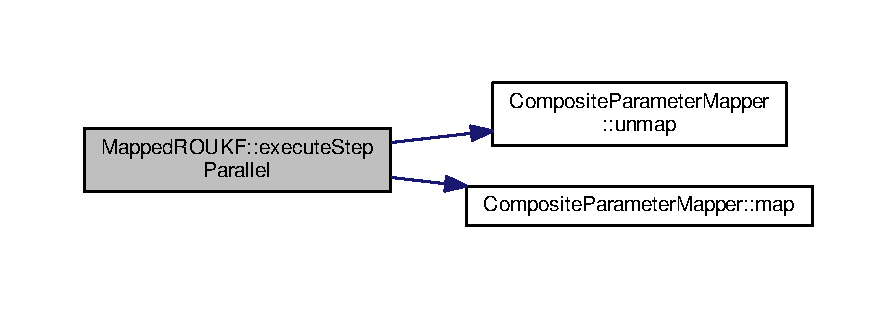
\includegraphics[width=350pt]{classMappedROUKF_ab6a3f488ef97ee3d8e11efa5aa0385c7_cgraph}
\end{center}
\end{figure}
\mbox{\Hypertarget{classMappedROUKF_aa6670e2cc9899b93b71db3f238ae93f3}\label{classMappedROUKF_aa6670e2cc9899b93b71db3f238ae93f3}} 
\index{Mapped\+R\+O\+U\+KF@{Mapped\+R\+O\+U\+KF}!get\+Parameters@{get\+Parameters}}
\index{get\+Parameters@{get\+Parameters}!Mapped\+R\+O\+U\+KF@{Mapped\+R\+O\+U\+KF}}
\subsubsection{\texorpdfstring{get\+Parameters()}{getParameters()}}
{\footnotesize\ttfamily void Mapped\+R\+O\+U\+K\+F\+::get\+Parameters (\begin{DoxyParamCaption}\item[{double $\ast$$\ast$}]{ThetaC }\end{DoxyParamCaption})\hspace{0.3cm}{\ttfamily [override]}, {\ttfamily [virtual]}}

Return the current parameter estimatives in the array {\ttfamily ThetaC}. 
\begin{DoxyParams}{Parameters}
{\em ThetaC} & Current parameter estimatives. \\
\hline
\end{DoxyParams}


Reimplemented from \mbox{\hyperlink{classAbstractROUKF_a1fa0b3e17f2618789dca9319bd755830}{Abstract\+R\+O\+U\+KF}}.



Definition at line 313 of file Mapped\+R\+O\+U\+K\+F.\+cpp.

Here is the call graph for this function\+:\nopagebreak
\begin{figure}[H]
\begin{center}
\leavevmode
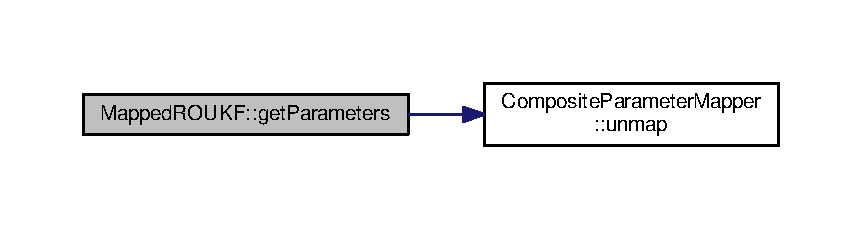
\includegraphics[width=350pt]{classMappedROUKF_aa6670e2cc9899b93b71db3f238ae93f3_cgraph}
\end{center}
\end{figure}
\mbox{\Hypertarget{classMappedROUKF_ad84ef097844217e5c5342e2ee8968521}\label{classMappedROUKF_ad84ef097844217e5c5342e2ee8968521}} 
\index{Mapped\+R\+O\+U\+KF@{Mapped\+R\+O\+U\+KF}!replace\+Mapper@{replace\+Mapper}}
\index{replace\+Mapper@{replace\+Mapper}!Mapped\+R\+O\+U\+KF@{Mapped\+R\+O\+U\+KF}}
\subsubsection{\texorpdfstring{replace\+Mapper()}{replaceMapper()}}
{\footnotesize\ttfamily void Mapped\+R\+O\+U\+K\+F\+::replace\+Mapper (\begin{DoxyParamCaption}\item[{\mbox{\hyperlink{classCompositeParameterMapper}{Composite\+Parameter\+Mapper}} $\ast$}]{mapper }\end{DoxyParamCaption})}

Replaces the current {\ttfamily mapper} for the new \mbox{\hyperlink{classCompositeParameterMapper}{Composite\+Parameter\+Mapper}} instance. 
\begin{DoxyParams}{Parameters}
{\em mapper} & New mapper instance. \\
\hline
\end{DoxyParams}


Definition at line 326 of file Mapped\+R\+O\+U\+K\+F.\+cpp.

Here is the call graph for this function\+:\nopagebreak
\begin{figure}[H]
\begin{center}
\leavevmode
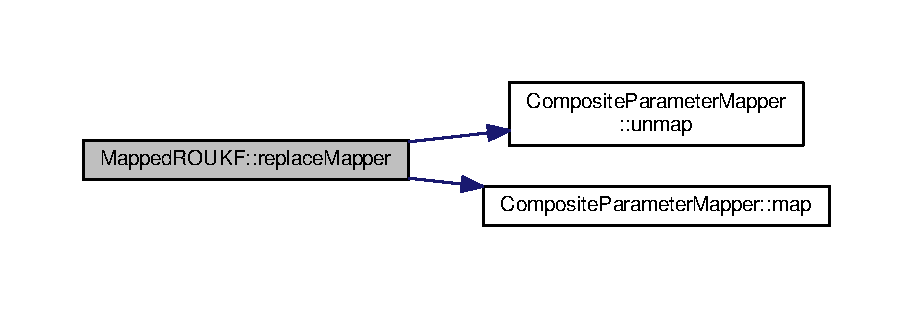
\includegraphics[width=350pt]{classMappedROUKF_ad84ef097844217e5c5342e2ee8968521_cgraph}
\end{center}
\end{figure}
\mbox{\Hypertarget{classMappedROUKF_ad4ddf881c1ade83fe0cc2ab99ad58b7e}\label{classMappedROUKF_ad4ddf881c1ade83fe0cc2ab99ad58b7e}} 
\index{Mapped\+R\+O\+U\+KF@{Mapped\+R\+O\+U\+KF}!reset@{reset}}
\index{reset@{reset}!Mapped\+R\+O\+U\+KF@{Mapped\+R\+O\+U\+KF}}
\subsubsection{\texorpdfstring{reset()}{reset()}}
{\footnotesize\ttfamily void Mapped\+R\+O\+U\+K\+F\+::reset (\begin{DoxyParamCaption}\item[{int}]{n\+Observations,  }\item[{int}]{n\+States,  }\item[{int}]{n\+Parameters,  }\item[{vector$<$ double $>$}]{observations\+Uncertainty,  }\item[{vector$<$ double $>$}]{parameters\+Uncertainty,  }\item[{\mbox{\hyperlink{classSigmaPointsGenerator_ad6f9474c0313425a10add120e0acf944}{Sigma\+Points\+Generator\+::\+S\+I\+G\+M\+A\+\_\+\+D\+I\+S\+T\+R\+I\+B\+U\+T\+I\+ON}}}]{sigma\+Distribution }\end{DoxyParamCaption})}

Returns to the initial state of the kalman filter. Not fully tested 
\begin{DoxyParams}{Parameters}
{\em n\+Observations} & Quantity of observations. \\
\hline
{\em n\+States} & Quantity of states. \\
\hline
{\em n\+Parameters} & Quantity of parameters. \\
\hline
{\em observations\+Uncertainty} & Vector with the uncertainty of each state in X. \\
\hline
{\em parameters\+Uncertainty} & Vector with the uncertainty of each parameter in Theta. \\
\hline
{\em sigma\+Distribution} & Type of sigmas applied to assess the unscented transform. \\
\hline
\end{DoxyParams}


Definition at line 286 of file Mapped\+R\+O\+U\+K\+F.\+cpp.

Here is the call graph for this function\+:\nopagebreak
\begin{figure}[H]
\begin{center}
\leavevmode
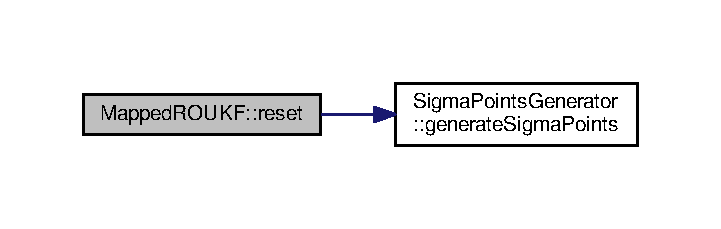
\includegraphics[width=346pt]{classMappedROUKF_ad4ddf881c1ade83fe0cc2ab99ad58b7e_cgraph}
\end{center}
\end{figure}
\mbox{\Hypertarget{classMappedROUKF_a4d3a109dc95812c8d9c6ac2a489349c2}\label{classMappedROUKF_a4d3a109dc95812c8d9c6ac2a489349c2}} 
\index{Mapped\+R\+O\+U\+KF@{Mapped\+R\+O\+U\+KF}!set\+Parameters@{set\+Parameters}}
\index{set\+Parameters@{set\+Parameters}!Mapped\+R\+O\+U\+KF@{Mapped\+R\+O\+U\+KF}}
\subsubsection{\texorpdfstring{set\+Parameters()}{setParameters()}}
{\footnotesize\ttfamily void Mapped\+R\+O\+U\+K\+F\+::set\+Parameters (\begin{DoxyParamCaption}\item[{double $\ast$}]{ThetaC }\end{DoxyParamCaption})\hspace{0.3cm}{\ttfamily [override]}, {\ttfamily [virtual]}}

Sets the initial parameter estimatives. 
\begin{DoxyParams}{Parameters}
{\em ThetaC} & Initial parameter estimatives. \\
\hline
\end{DoxyParams}


Reimplemented from \mbox{\hyperlink{classAbstractROUKF_a8e8f7c34007a2363530f7cca4cfb0c9f}{Abstract\+R\+O\+U\+KF}}.



Definition at line 320 of file Mapped\+R\+O\+U\+K\+F.\+cpp.

Here is the call graph for this function\+:\nopagebreak
\begin{figure}[H]
\begin{center}
\leavevmode
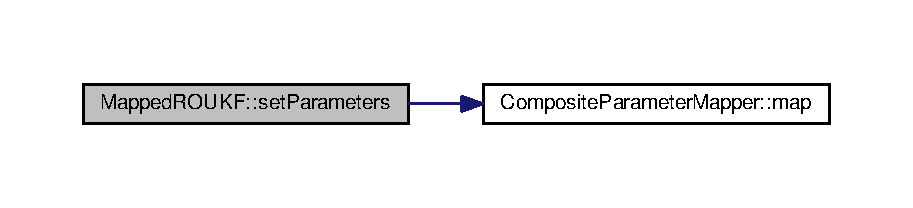
\includegraphics[width=350pt]{classMappedROUKF_a4d3a109dc95812c8d9c6ac2a489349c2_cgraph}
\end{center}
\end{figure}


\subsection{Member Data Documentation}
\mbox{\Hypertarget{classMappedROUKF_a5177d0749fa9a6ce81d760267f4e7e09}\label{classMappedROUKF_a5177d0749fa9a6ce81d760267f4e7e09}} 
\index{Mapped\+R\+O\+U\+KF@{Mapped\+R\+O\+U\+KF}!mapper@{mapper}}
\index{mapper@{mapper}!Mapped\+R\+O\+U\+KF@{Mapped\+R\+O\+U\+KF}}
\subsubsection{\texorpdfstring{mapper}{mapper}}
{\footnotesize\ttfamily \mbox{\hyperlink{classCompositeParameterMapper}{Composite\+Parameter\+Mapper}}$\ast$ Mapped\+R\+O\+U\+K\+F\+::mapper\hspace{0.3cm}{\ttfamily [private]}}

Mapping function between the problem parameters and the kalman parameters. 

Definition at line 60 of file Mapped\+R\+O\+U\+K\+F.\+h.



The documentation for this class was generated from the following files\+:\begin{DoxyCompactItemize}
\item 
Mapped\+R\+O\+U\+K\+F.\+h\item 
Mapped\+R\+O\+U\+K\+F.\+cpp\end{DoxyCompactItemize}

\hypertarget{classROUKF}{}\section{R\+O\+U\+KF Class Reference}
\label{classROUKF}\index{R\+O\+U\+KF@{R\+O\+U\+KF}}


{\ttfamily \#include $<$R\+O\+U\+K\+F.\+h$>$}



Inheritance diagram for R\+O\+U\+KF\+:\nopagebreak
\begin{figure}[H]
\begin{center}
\leavevmode
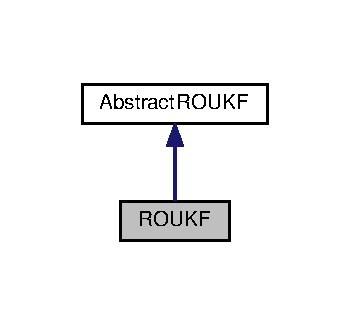
\includegraphics[width=168pt]{classROUKF__inherit__graph}
\end{center}
\end{figure}


Collaboration diagram for R\+O\+U\+KF\+:\nopagebreak
\begin{figure}[H]
\begin{center}
\leavevmode
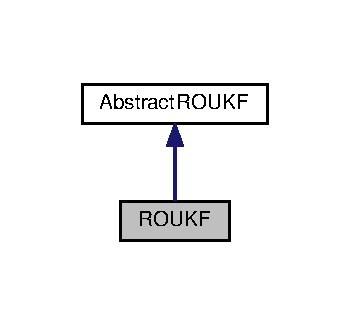
\includegraphics[width=168pt]{classROUKF__coll__graph}
\end{center}
\end{figure}
\subsection*{Public Member Functions}
\begin{DoxyCompactItemize}
\item 
\mbox{\hyperlink{classROUKF_a16fd0fbe99e00745254f56052ad44f3f}{R\+O\+U\+KF}} (int \mbox{\hyperlink{classAbstractROUKF_a4f6403f7fd2fac691e4ac516f47c0a06}{n\+Observations}}, int \mbox{\hyperlink{classAbstractROUKF_af9ce480feb5d97761f20fdd546878aff}{n\+States}}, int \mbox{\hyperlink{classAbstractROUKF_a488f708dcdd66758cd879421cd454846}{n\+Parameters}}, double $\ast$states\+Uncertainty, double $\ast$parameters\+Uncertainty, \mbox{\hyperlink{classSigmaPointsGenerator_ad6f9474c0313425a10add120e0acf944}{Sigma\+Points\+Generator\+::\+S\+I\+G\+M\+A\+\_\+\+D\+I\+S\+T\+R\+I\+B\+U\+T\+I\+ON}} sigma\+Distribution)
\item 
\mbox{\hyperlink{classROUKF_aefba1ab1ab07bed45f43897c19f4f0a2}{$\sim$\+R\+O\+U\+KF}} ()
\item 
double \mbox{\hyperlink{classROUKF_ad200c0176a1e6e443fbea55bd8905dd6}{execute\+Step}} (double $\ast$Zkhatc, forward\+Op A, observation\+Op H)
\item 
double \mbox{\hyperlink{classROUKF_a0494bdc8ad1870dabb80581794dccc58}{execute\+Step\+Parallel}} (double $\ast$Zkhatc, forward\+Op A, observation\+Op H, int seed, M\+P\+I\+\_\+\+Comm local\+\_\+comm, M\+P\+I\+\_\+\+Comm masters\+\_\+comm)
\item 
void \mbox{\hyperlink{classROUKF_add2b1ded99b16046f706557a2129d41a}{reset}} (int \mbox{\hyperlink{classAbstractROUKF_a4f6403f7fd2fac691e4ac516f47c0a06}{n\+Observations}}, int \mbox{\hyperlink{classAbstractROUKF_af9ce480feb5d97761f20fdd546878aff}{n\+States}}, int \mbox{\hyperlink{classAbstractROUKF_a488f708dcdd66758cd879421cd454846}{n\+Parameters}}, double $\ast$states\+Uncertainty, double $\ast$parameters\+Uncertainty, \mbox{\hyperlink{classSigmaPointsGenerator_ad6f9474c0313425a10add120e0acf944}{Sigma\+Points\+Generator\+::\+S\+I\+G\+M\+A\+\_\+\+D\+I\+S\+T\+R\+I\+B\+U\+T\+I\+ON}} sigma\+Distribution)
\end{DoxyCompactItemize}
\subsection*{Additional Inherited Members}


\subsection{Detailed Description}
An example for the usage of the library\+:


\begin{DoxyCode}
   int (*ptA)(\textcolor{keywordtype}{double}*, int) = NULL;
void (*ptH)(\textcolor{keywordtype}{double}*, int, \textcolor{keywordtype}{double}*, int) = NULL;
ptA = \&forwardOpElasticity;
ptH = \&observerOpElasticity;

 \textcolor{comment}{//    Initialization parameters}
\textcolor{keywordflow}{for} (\textcolor{keywordtype}{int} i = 0; i < \mbox{\hyperlink{classAbstractROUKF_a488f708dcdd66758cd879421cd454846}{nParameters}}; i++) \{
   initialGuess[i] = 2.5E5;            \textcolor{comment}{// -> X0}
   parametersUncertainties[i] =1E8;    \textcolor{comment}{// -> U0^\{-1\}}
\}
\mbox{\hyperlink{classROUKF}{ROUKF}} *kalmanInstance = \textcolor{keyword}{new} \mbox{\hyperlink{classROUKF_a16fd0fbe99e00745254f56052ad44f3f}{ROUKF}}(\mbox{\hyperlink{classAbstractROUKF_af9ce480feb5d97761f20fdd546878aff}{nStates}}, \mbox{\hyperlink{classAbstractROUKF_a488f708dcdd66758cd879421cd454846}{nParameters}}, statesUncertainties,
parametersUncertainties);

\textcolor{comment}{// Set initial condition}
kalmanInstance->\mbox{\hyperlink{classAbstractROUKF_a618f4719892c0997e5f62cc23913aa12}{setState}}(initialGuess, \mbox{\hyperlink{classAbstractROUKF_a488f708dcdd66758cd879421cd454846}{nParameters}});

\textcolor{keywordflow}{for} (\textcolor{keywordtype}{int} it = 0; it < 3000; it++) \{
   \mbox{\hyperlink{classAbstractROUKF_a551d0b61b010efe7923358c93cbd0db5}{error}} = kalmanInstance->\mbox{\hyperlink{classROUKF_ad200c0176a1e6e443fbea55bd8905dd6}{executeStep}}(observation, \mbox{\hyperlink{classAbstractROUKF_af9ce480feb5d97761f20fdd546878aff}{nStates}}, ptA, ptH);
\}

\textcolor{comment}{// Get the Kalman estimation}
kalmanInstance->\mbox{\hyperlink{classAbstractROUKF_ad24dafa1f4cb02a38958264740588b87}{getState}}(\&sol);            \textcolor{comment}{// -> XSol}
\end{DoxyCode}
 Class that implements the reduced order unscented Kalman filter. 

Definition at line 56 of file R\+O\+U\+K\+F.\+h.



\subsection{Constructor \& Destructor Documentation}
\mbox{\Hypertarget{classROUKF_a16fd0fbe99e00745254f56052ad44f3f}\label{classROUKF_a16fd0fbe99e00745254f56052ad44f3f}} 
\index{R\+O\+U\+KF@{R\+O\+U\+KF}!R\+O\+U\+KF@{R\+O\+U\+KF}}
\index{R\+O\+U\+KF@{R\+O\+U\+KF}!R\+O\+U\+KF@{R\+O\+U\+KF}}
\subsubsection{\texorpdfstring{R\+O\+U\+K\+F()}{ROUKF()}}
{\footnotesize\ttfamily R\+O\+U\+K\+F\+::\+R\+O\+U\+KF (\begin{DoxyParamCaption}\item[{int}]{n\+Observations,  }\item[{int}]{n\+States,  }\item[{int}]{n\+Parameters,  }\item[{double $\ast$}]{states\+Uncertainty,  }\item[{double $\ast$}]{parameters\+Uncertainty,  }\item[{\mbox{\hyperlink{classSigmaPointsGenerator_ad6f9474c0313425a10add120e0acf944}{Sigma\+Points\+Generator\+::\+S\+I\+G\+M\+A\+\_\+\+D\+I\+S\+T\+R\+I\+B\+U\+T\+I\+ON}}}]{sigma\+Distribution }\end{DoxyParamCaption})}

Creates the covariance matrixes and sigma points associated with the extended vector X and their uncertainty. 
\begin{DoxyParams}{Parameters}
{\em n\+Observations} & Quantity of observations. \\
\hline
{\em n\+States} & Quantity of states. \\
\hline
{\em n\+Parameters} & Quantity of parameters. \\
\hline
{\em states\+Uncertainty} & Vector with the uncertainty of each state in X. \\
\hline
{\em parameters\+Uncertainty} & Vector with the uncertainty of each parameter in Theta. \\
\hline
{\em sigma\+Distribution} & Type of sigmas applied to assess the unscented transform. \\
\hline
\end{DoxyParams}


Definition at line 12 of file R\+O\+U\+K\+F.\+cpp.

Here is the call graph for this function\+:\nopagebreak
\begin{figure}[H]
\begin{center}
\leavevmode
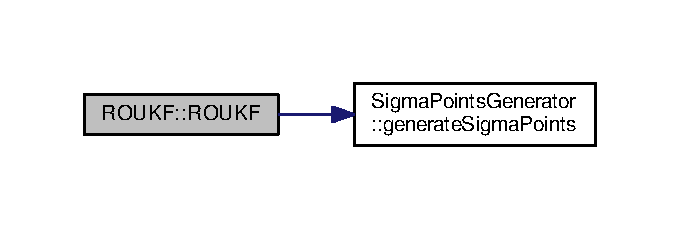
\includegraphics[width=326pt]{classROUKF_a16fd0fbe99e00745254f56052ad44f3f_cgraph}
\end{center}
\end{figure}
\mbox{\Hypertarget{classROUKF_aefba1ab1ab07bed45f43897c19f4f0a2}\label{classROUKF_aefba1ab1ab07bed45f43897c19f4f0a2}} 
\index{R\+O\+U\+KF@{R\+O\+U\+KF}!````~R\+O\+U\+KF@{$\sim$\+R\+O\+U\+KF}}
\index{````~R\+O\+U\+KF@{$\sim$\+R\+O\+U\+KF}!R\+O\+U\+KF@{R\+O\+U\+KF}}
\subsubsection{\texorpdfstring{$\sim$\+R\+O\+U\+K\+F()}{~ROUKF()}}
{\footnotesize\ttfamily R\+O\+U\+K\+F\+::$\sim$\+R\+O\+U\+KF (\begin{DoxyParamCaption}{ }\end{DoxyParamCaption})}

Void destructor. 

Definition at line 41 of file R\+O\+U\+K\+F.\+cpp.



\subsection{Member Function Documentation}
\mbox{\Hypertarget{classROUKF_ad200c0176a1e6e443fbea55bd8905dd6}\label{classROUKF_ad200c0176a1e6e443fbea55bd8905dd6}} 
\index{R\+O\+U\+KF@{R\+O\+U\+KF}!execute\+Step@{execute\+Step}}
\index{execute\+Step@{execute\+Step}!R\+O\+U\+KF@{R\+O\+U\+KF}}
\subsubsection{\texorpdfstring{execute\+Step()}{executeStep()}}
{\footnotesize\ttfamily double R\+O\+U\+K\+F\+::execute\+Step (\begin{DoxyParamCaption}\item[{double $\ast$}]{Zkhatc,  }\item[{forward\+Op}]{A,  }\item[{observation\+Op}]{H }\end{DoxyParamCaption})}

Performs one step of the Kalman filtering process in serial execution of the sigma points. 
\begin{DoxyParams}{Parameters}
{\em Zkhatc} & Current observations estimations. \\
\hline
{\em A} & Forward operator. \\
\hline
{\em H} & Observation operator; \\
\hline
\end{DoxyParams}
\begin{DoxyReturn}{Returns}
Current L2 norm of the errors across all observations. 
\end{DoxyReturn}


Definition at line 44 of file R\+O\+U\+K\+F.\+cpp.

\mbox{\Hypertarget{classROUKF_a0494bdc8ad1870dabb80581794dccc58}\label{classROUKF_a0494bdc8ad1870dabb80581794dccc58}} 
\index{R\+O\+U\+KF@{R\+O\+U\+KF}!execute\+Step\+Parallel@{execute\+Step\+Parallel}}
\index{execute\+Step\+Parallel@{execute\+Step\+Parallel}!R\+O\+U\+KF@{R\+O\+U\+KF}}
\subsubsection{\texorpdfstring{execute\+Step\+Parallel()}{executeStepParallel()}}
{\footnotesize\ttfamily double R\+O\+U\+K\+F\+::execute\+Step\+Parallel (\begin{DoxyParamCaption}\item[{double $\ast$}]{Zkhatc,  }\item[{forward\+Op}]{A,  }\item[{observation\+Op}]{H,  }\item[{int}]{seed,  }\item[{M\+P\+I\+\_\+\+Comm}]{local\+\_\+comm,  }\item[{M\+P\+I\+\_\+\+Comm}]{masters\+\_\+comm }\end{DoxyParamCaption})}

Performs one step of the Kalman filtering process with parallel execution of the sigma points. 
\begin{DoxyParams}{Parameters}
{\em Zkhatc} & Current observations estimations. \\
\hline
{\em A} & Forward operator. \\
\hline
{\em H} & Observation operator; \\
\hline
{\em seed} & Sigma point ID for the current M\+PI process. \\
\hline
{\em local\+\_\+comm} & Communicator of all M\+PI processes that solve the sigma point {\ttfamily seed}. \\
\hline
{\em masters\+\_\+comm} & Communicator of the master M\+PI processes of each sigma point {\ttfamily seed}. \\
\hline
\end{DoxyParams}
\begin{DoxyReturn}{Returns}
Current L2 norm of the errors across all observations. 
\end{DoxyReturn}


Definition at line 119 of file R\+O\+U\+K\+F.\+cpp.

\mbox{\Hypertarget{classROUKF_add2b1ded99b16046f706557a2129d41a}\label{classROUKF_add2b1ded99b16046f706557a2129d41a}} 
\index{R\+O\+U\+KF@{R\+O\+U\+KF}!reset@{reset}}
\index{reset@{reset}!R\+O\+U\+KF@{R\+O\+U\+KF}}
\subsubsection{\texorpdfstring{reset()}{reset()}}
{\footnotesize\ttfamily void R\+O\+U\+K\+F\+::reset (\begin{DoxyParamCaption}\item[{int}]{n\+Observations,  }\item[{int}]{n\+States,  }\item[{int}]{n\+Parameters,  }\item[{double $\ast$}]{states\+Uncertainty,  }\item[{double $\ast$}]{parameters\+Uncertainty,  }\item[{\mbox{\hyperlink{classSigmaPointsGenerator_ad6f9474c0313425a10add120e0acf944}{Sigma\+Points\+Generator\+::\+S\+I\+G\+M\+A\+\_\+\+D\+I\+S\+T\+R\+I\+B\+U\+T\+I\+ON}}}]{sigma\+Distribution }\end{DoxyParamCaption})}

Returns to the initial state of the kalman filter. Not fully tested 
\begin{DoxyParams}{Parameters}
{\em n\+Observations} & Quantity of observations. \\
\hline
{\em n\+States} & Quantity of states. \\
\hline
{\em n\+Parameters} & Quantity of parameters. \\
\hline
{\em states\+Uncertainty} & Vector with the uncertainty of each state in X. \\
\hline
{\em parameters\+Uncertainty} & Vector with the uncertainty of each parameter in Theta. \\
\hline
{\em sigma\+Distribution} & Type of sigmas applied to assess the unscented transform. \\
\hline
\end{DoxyParams}


Definition at line 210 of file R\+O\+U\+K\+F.\+cpp.

Here is the call graph for this function\+:\nopagebreak
\begin{figure}[H]
\begin{center}
\leavevmode
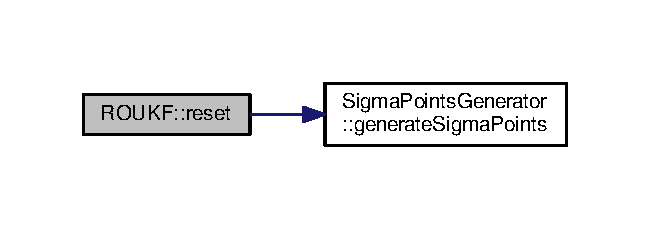
\includegraphics[width=312pt]{classROUKF_add2b1ded99b16046f706557a2129d41a_cgraph}
\end{center}
\end{figure}


The documentation for this class was generated from the following files\+:\begin{DoxyCompactItemize}
\item 
R\+O\+U\+K\+F.\+h\item 
R\+O\+U\+K\+F.\+cpp\end{DoxyCompactItemize}

\hypertarget{classSigmaPointsGenerator}{}\section{Sigma\+Points\+Generator Class Reference}
\label{classSigmaPointsGenerator}\index{Sigma\+Points\+Generator@{Sigma\+Points\+Generator}}


{\ttfamily \#include $<$Sigma\+Points\+Generator.\+h$>$}

\subsection*{Public Types}
\begin{DoxyCompactItemize}
\item 
enum \mbox{\hyperlink{classSigmaPointsGenerator_ad6f9474c0313425a10add120e0acf944}{S\+I\+G\+M\+A\+\_\+\+D\+I\+S\+T\+R\+I\+B\+U\+T\+I\+ON}} \{ {\bfseries S\+I\+M\+P\+L\+EX}, 
{\bfseries C\+A\+N\+O\+N\+IC}, 
{\bfseries S\+T\+AR}, 
{\bfseries S\+I\+M\+P\+L\+E\+X\+\_\+\+S\+T\+AR}
 \}
\end{DoxyCompactItemize}
\subsection*{Static Public Member Functions}
\begin{DoxyCompactItemize}
\item 
static void \mbox{\hyperlink{classSigmaPointsGenerator_a72a2e6479c0d9e458bad143ea67093ba}{generate\+Sigma\+Points}} (int n\+Parameters, \mbox{\hyperlink{classSigmaPointsGenerator_ad6f9474c0313425a10add120e0acf944}{S\+I\+G\+M\+A\+\_\+\+D\+I\+S\+T\+R\+I\+B\+U\+T\+I\+ON}} distribution, arma\+::mat $\ast$sigma)
\end{DoxyCompactItemize}
\subsection*{Static Protected Member Functions}
\begin{DoxyCompactItemize}
\item 
static void \mbox{\hyperlink{classSigmaPointsGenerator_a9c6bab6d0253b217488a04d65853e585}{canonic\+Sigma\+Points}} (int n\+Parameters, arma\+::mat $\ast$sigma)
\item 
static void \mbox{\hyperlink{classSigmaPointsGenerator_a565e88c8abc4d82fc4c6aed75f9693a9}{simplex\+Sigma\+Points}} (int n\+Parameters, arma\+::mat $\ast$sigma)
\item 
static void \mbox{\hyperlink{classSigmaPointsGenerator_a4187ef53aff978a7f2874533ce2fb0f1}{star\+Sigma\+Points}} (int n\+Parameters, arma\+::mat $\ast$sigma)
\item 
static void \mbox{\hyperlink{classSigmaPointsGenerator_aecd82749d0e9865e6abfb9b8410b9542}{simplex\+Star\+Sigma\+Points}} (int n\+Parameters, arma\+::mat $\ast$sigma)
\end{DoxyCompactItemize}
\subsection*{Static Private Member Functions}
\begin{DoxyCompactItemize}
\item 
static arma\+::mat \mbox{\hyperlink{classSigmaPointsGenerator_a5cfc30f689336a2a736e8c02fdaccfd2}{get\+Simplex\+Sigma\+Points}} (int n\+Points, double weight)
\end{DoxyCompactItemize}


\subsection{Detailed Description}
Static class which generates different distributions of sigma points. 

Definition at line 16 of file Sigma\+Points\+Generator.\+h.



\subsection{Member Enumeration Documentation}
\mbox{\Hypertarget{classSigmaPointsGenerator_ad6f9474c0313425a10add120e0acf944}\label{classSigmaPointsGenerator_ad6f9474c0313425a10add120e0acf944}} 
\index{Sigma\+Points\+Generator@{Sigma\+Points\+Generator}!S\+I\+G\+M\+A\+\_\+\+D\+I\+S\+T\+R\+I\+B\+U\+T\+I\+ON@{S\+I\+G\+M\+A\+\_\+\+D\+I\+S\+T\+R\+I\+B\+U\+T\+I\+ON}}
\index{S\+I\+G\+M\+A\+\_\+\+D\+I\+S\+T\+R\+I\+B\+U\+T\+I\+ON@{S\+I\+G\+M\+A\+\_\+\+D\+I\+S\+T\+R\+I\+B\+U\+T\+I\+ON}!Sigma\+Points\+Generator@{Sigma\+Points\+Generator}}
\subsubsection{\texorpdfstring{S\+I\+G\+M\+A\+\_\+\+D\+I\+S\+T\+R\+I\+B\+U\+T\+I\+ON}{SIGMA\_DISTRIBUTION}}
{\footnotesize\ttfamily enum \mbox{\hyperlink{classSigmaPointsGenerator_ad6f9474c0313425a10add120e0acf944}{Sigma\+Points\+Generator\+::\+S\+I\+G\+M\+A\+\_\+\+D\+I\+S\+T\+R\+I\+B\+U\+T\+I\+ON}}}

Enumeration for the different kinds of sigma points distributions. 

Definition at line 19 of file Sigma\+Points\+Generator.\+h.



\subsection{Member Function Documentation}
\mbox{\Hypertarget{classSigmaPointsGenerator_a9c6bab6d0253b217488a04d65853e585}\label{classSigmaPointsGenerator_a9c6bab6d0253b217488a04d65853e585}} 
\index{Sigma\+Points\+Generator@{Sigma\+Points\+Generator}!canonic\+Sigma\+Points@{canonic\+Sigma\+Points}}
\index{canonic\+Sigma\+Points@{canonic\+Sigma\+Points}!Sigma\+Points\+Generator@{Sigma\+Points\+Generator}}
\subsubsection{\texorpdfstring{canonic\+Sigma\+Points()}{canonicSigmaPoints()}}
{\footnotesize\ttfamily void Sigma\+Points\+Generator\+::canonic\+Sigma\+Points (\begin{DoxyParamCaption}\item[{int}]{n\+Parameters,  }\item[{arma\+::mat $\ast$}]{sigma }\end{DoxyParamCaption})\hspace{0.3cm}{\ttfamily [static]}, {\ttfamily [protected]}}

Canonic sigma points (2 points per parameter symmetrics to the centroid.) 
\begin{DoxyParams}{Parameters}
{\em n\+Parameters} & Quantity of parameters \\
\hline
{\em sigma} & Output matrix with one sigma point per column. \\
\hline
\end{DoxyParams}


Definition at line 34 of file Sigma\+Points\+Generator.\+cpp.

\mbox{\Hypertarget{classSigmaPointsGenerator_a72a2e6479c0d9e458bad143ea67093ba}\label{classSigmaPointsGenerator_a72a2e6479c0d9e458bad143ea67093ba}} 
\index{Sigma\+Points\+Generator@{Sigma\+Points\+Generator}!generate\+Sigma\+Points@{generate\+Sigma\+Points}}
\index{generate\+Sigma\+Points@{generate\+Sigma\+Points}!Sigma\+Points\+Generator@{Sigma\+Points\+Generator}}
\subsubsection{\texorpdfstring{generate\+Sigma\+Points()}{generateSigmaPoints()}}
{\footnotesize\ttfamily void Sigma\+Points\+Generator\+::generate\+Sigma\+Points (\begin{DoxyParamCaption}\item[{int}]{n\+Parameters,  }\item[{\mbox{\hyperlink{classSigmaPointsGenerator_ad6f9474c0313425a10add120e0acf944}{S\+I\+G\+M\+A\+\_\+\+D\+I\+S\+T\+R\+I\+B\+U\+T\+I\+ON}}}]{distribution,  }\item[{arma\+::mat $\ast$}]{sigma }\end{DoxyParamCaption})\hspace{0.3cm}{\ttfamily [static]}}

Generates the matrix sigma where each column is a sigma point of the type {\ttfamily distribution}. 
\begin{DoxyParams}{Parameters}
{\em n\+Parameters} & Quantity of parameters to estimate. \\
\hline
{\em distribution} & Type of distribution used to generate the sigma points. \\
\hline
{\em sigma} & Output matrix with one sigma point per column. \\
\hline
\end{DoxyParams}


Definition at line 12 of file Sigma\+Points\+Generator.\+cpp.

\mbox{\Hypertarget{classSigmaPointsGenerator_a5cfc30f689336a2a736e8c02fdaccfd2}\label{classSigmaPointsGenerator_a5cfc30f689336a2a736e8c02fdaccfd2}} 
\index{Sigma\+Points\+Generator@{Sigma\+Points\+Generator}!get\+Simplex\+Sigma\+Points@{get\+Simplex\+Sigma\+Points}}
\index{get\+Simplex\+Sigma\+Points@{get\+Simplex\+Sigma\+Points}!Sigma\+Points\+Generator@{Sigma\+Points\+Generator}}
\subsubsection{\texorpdfstring{get\+Simplex\+Sigma\+Points()}{getSimplexSigmaPoints()}}
{\footnotesize\ttfamily arma\+::mat Sigma\+Points\+Generator\+::get\+Simplex\+Sigma\+Points (\begin{DoxyParamCaption}\item[{int}]{n\+Points,  }\item[{double}]{weight }\end{DoxyParamCaption})\hspace{0.3cm}{\ttfamily [static]}, {\ttfamily [private]}}

Recursive generation of simplex sigma points. 
\begin{DoxyParams}{Parameters}
{\em n\+Points} & Quantity of points to generate. \\
\hline
{\em weight} & Weight for the current generated points. \\
\hline
\end{DoxyParams}
\begin{DoxyReturn}{Returns}
Matrix of sigma points. 
\end{DoxyReturn}


Definition at line 64 of file Sigma\+Points\+Generator.\+cpp.

\mbox{\Hypertarget{classSigmaPointsGenerator_a565e88c8abc4d82fc4c6aed75f9693a9}\label{classSigmaPointsGenerator_a565e88c8abc4d82fc4c6aed75f9693a9}} 
\index{Sigma\+Points\+Generator@{Sigma\+Points\+Generator}!simplex\+Sigma\+Points@{simplex\+Sigma\+Points}}
\index{simplex\+Sigma\+Points@{simplex\+Sigma\+Points}!Sigma\+Points\+Generator@{Sigma\+Points\+Generator}}
\subsubsection{\texorpdfstring{simplex\+Sigma\+Points()}{simplexSigmaPoints()}}
{\footnotesize\ttfamily void Sigma\+Points\+Generator\+::simplex\+Sigma\+Points (\begin{DoxyParamCaption}\item[{int}]{n\+Parameters,  }\item[{arma\+::mat $\ast$}]{sigma }\end{DoxyParamCaption})\hspace{0.3cm}{\ttfamily [static]}, {\ttfamily [protected]}}

Simplex sigma points. 
\begin{DoxyParams}{Parameters}
{\em n\+Parameters} & Quantity of parameters \\
\hline
{\em sigma} & Output matrix with one sigma point per column. \\
\hline
\end{DoxyParams}


Definition at line 47 of file Sigma\+Points\+Generator.\+cpp.

\mbox{\Hypertarget{classSigmaPointsGenerator_aecd82749d0e9865e6abfb9b8410b9542}\label{classSigmaPointsGenerator_aecd82749d0e9865e6abfb9b8410b9542}} 
\index{Sigma\+Points\+Generator@{Sigma\+Points\+Generator}!simplex\+Star\+Sigma\+Points@{simplex\+Star\+Sigma\+Points}}
\index{simplex\+Star\+Sigma\+Points@{simplex\+Star\+Sigma\+Points}!Sigma\+Points\+Generator@{Sigma\+Points\+Generator}}
\subsubsection{\texorpdfstring{simplex\+Star\+Sigma\+Points()}{simplexStarSigmaPoints()}}
{\footnotesize\ttfamily void Sigma\+Points\+Generator\+::simplex\+Star\+Sigma\+Points (\begin{DoxyParamCaption}\item[{int}]{n\+Parameters,  }\item[{arma\+::mat $\ast$}]{sigma }\end{DoxyParamCaption})\hspace{0.3cm}{\ttfamily [static]}, {\ttfamily [protected]}}

Same as simplex sigma points with an additional point at the centroid. 
\begin{DoxyParams}{Parameters}
{\em n\+Parameters} & Quantity of parameters \\
\hline
{\em sigma} & Output matrix with one sigma point per column. \\
\hline
\end{DoxyParams}


Definition at line 85 of file Sigma\+Points\+Generator.\+cpp.

\mbox{\Hypertarget{classSigmaPointsGenerator_a4187ef53aff978a7f2874533ce2fb0f1}\label{classSigmaPointsGenerator_a4187ef53aff978a7f2874533ce2fb0f1}} 
\index{Sigma\+Points\+Generator@{Sigma\+Points\+Generator}!star\+Sigma\+Points@{star\+Sigma\+Points}}
\index{star\+Sigma\+Points@{star\+Sigma\+Points}!Sigma\+Points\+Generator@{Sigma\+Points\+Generator}}
\subsubsection{\texorpdfstring{star\+Sigma\+Points()}{starSigmaPoints()}}
{\footnotesize\ttfamily void Sigma\+Points\+Generator\+::star\+Sigma\+Points (\begin{DoxyParamCaption}\item[{int}]{n\+Parameters,  }\item[{arma\+::mat $\ast$}]{sigma }\end{DoxyParamCaption})\hspace{0.3cm}{\ttfamily [static]}, {\ttfamily [protected]}}

Same as canonic sigma points with an additional point at the centroid. 
\begin{DoxyParams}{Parameters}
{\em n\+Parameters} & Quantity of parameters \\
\hline
{\em sigma} & Output matrix with one sigma point per column. \\
\hline
\end{DoxyParams}


Definition at line 52 of file Sigma\+Points\+Generator.\+cpp.



The documentation for this class was generated from the following files\+:\begin{DoxyCompactItemize}
\item 
Sigma\+Points\+Generator.\+h\item 
Sigma\+Points\+Generator.\+cpp\end{DoxyCompactItemize}

\hypertarget{classSigmoidParameterMapper}{}\section{Sigmoid\+Parameter\+Mapper Class Reference}
\label{classSigmoidParameterMapper}\index{Sigmoid\+Parameter\+Mapper@{Sigmoid\+Parameter\+Mapper}}


{\ttfamily \#include $<$Sigmoid\+Parameter\+Mapper.\+h$>$}



Inheritance diagram for Sigmoid\+Parameter\+Mapper\+:\nopagebreak
\begin{figure}[H]
\begin{center}
\leavevmode
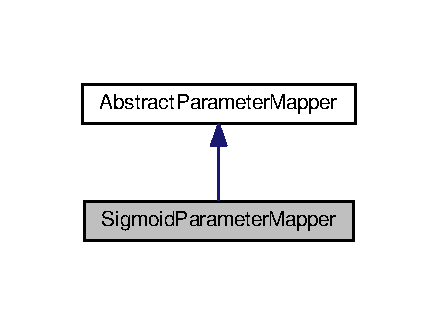
\includegraphics[width=210pt]{classSigmoidParameterMapper__inherit__graph}
\end{center}
\end{figure}


Collaboration diagram for Sigmoid\+Parameter\+Mapper\+:\nopagebreak
\begin{figure}[H]
\begin{center}
\leavevmode
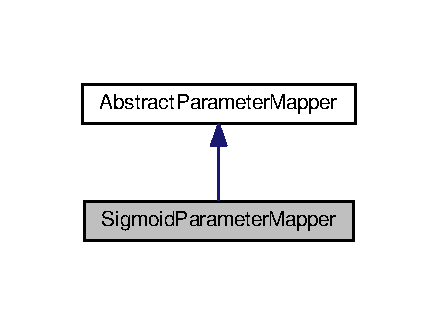
\includegraphics[width=210pt]{classSigmoidParameterMapper__coll__graph}
\end{center}
\end{figure}
\subsection*{Public Member Functions}
\begin{DoxyCompactItemize}
\item 
\mbox{\hyperlink{classSigmoidParameterMapper_a1f39049fb6a69ae650161d52158a2f10}{Sigmoid\+Parameter\+Mapper}} (double \mbox{\hyperlink{classSigmoidParameterMapper_a55543b10e333cbe122bef3fdffbe1bf9}{min}}, double \mbox{\hyperlink{classSigmoidParameterMapper_a87e681e19a32deadc0231f979636ad17}{max}})
\item 
vector$<$ double $>$ \mbox{\hyperlink{classSigmoidParameterMapper_a808db49587ff6c2d2c2b2efc84de80f6}{map}} (vector$<$ double $>$ problem\+Parameters)
\item 
vector$<$ double $>$ \mbox{\hyperlink{classSigmoidParameterMapper_a5b7031c2945f69130e0423427525e256}{unmap}} (vector$<$ double $>$ kalman\+Parameters)
\end{DoxyCompactItemize}
\subsection*{Private Attributes}
\begin{DoxyCompactItemize}
\item 
double \mbox{\hyperlink{classSigmoidParameterMapper_a55543b10e333cbe122bef3fdffbe1bf9}{min}}
\item 
double \mbox{\hyperlink{classSigmoidParameterMapper_a87e681e19a32deadc0231f979636ad17}{max}}
\end{DoxyCompactItemize}


\subsection{Detailed Description}
Implementation of the \mbox{\hyperlink{classAbstractParameterMapper}{Abstract\+Parameter\+Mapper}} class that map the problem parameters into the kalman parameters using a sigmoid function with a user preseted range. 

Definition at line 17 of file Sigmoid\+Parameter\+Mapper.\+h.



\subsection{Constructor \& Destructor Documentation}
\mbox{\Hypertarget{classSigmoidParameterMapper_a1f39049fb6a69ae650161d52158a2f10}\label{classSigmoidParameterMapper_a1f39049fb6a69ae650161d52158a2f10}} 
\index{Sigmoid\+Parameter\+Mapper@{Sigmoid\+Parameter\+Mapper}!Sigmoid\+Parameter\+Mapper@{Sigmoid\+Parameter\+Mapper}}
\index{Sigmoid\+Parameter\+Mapper@{Sigmoid\+Parameter\+Mapper}!Sigmoid\+Parameter\+Mapper@{Sigmoid\+Parameter\+Mapper}}
\subsubsection{\texorpdfstring{Sigmoid\+Parameter\+Mapper()}{SigmoidParameterMapper()}}
{\footnotesize\ttfamily Sigmoid\+Parameter\+Mapper\+::\+Sigmoid\+Parameter\+Mapper (\begin{DoxyParamCaption}\item[{double}]{min,  }\item[{double}]{max }\end{DoxyParamCaption})}

Constructor that sets the range of mapping to (min,max) 
\begin{DoxyParams}{Parameters}
{\em min} & Minimum value in the problem parameters range. \\
\hline
{\em max} & Maximum value in the problem parameters range. \\
\hline
\end{DoxyParams}


Definition at line 12 of file Sigmoid\+Parameter\+Mapper.\+cpp.



\subsection{Member Function Documentation}
\mbox{\Hypertarget{classSigmoidParameterMapper_a808db49587ff6c2d2c2b2efc84de80f6}\label{classSigmoidParameterMapper_a808db49587ff6c2d2c2b2efc84de80f6}} 
\index{Sigmoid\+Parameter\+Mapper@{Sigmoid\+Parameter\+Mapper}!map@{map}}
\index{map@{map}!Sigmoid\+Parameter\+Mapper@{Sigmoid\+Parameter\+Mapper}}
\subsubsection{\texorpdfstring{map()}{map()}}
{\footnotesize\ttfamily vector$<$ double $>$ Sigmoid\+Parameter\+Mapper\+::map (\begin{DoxyParamCaption}\item[{vector$<$ double $>$}]{problem\+Parameters }\end{DoxyParamCaption})\hspace{0.3cm}{\ttfamily [virtual]}}

Maps the problem parameters into the space of parameters where kalman filter optimize them. 
\begin{DoxyParams}{Parameters}
{\em problem\+Parameters} & Set of problem parameters. \\
\hline
\end{DoxyParams}
\begin{DoxyReturn}{Returns}
Set of kalman parameters 
\end{DoxyReturn}


Implements \mbox{\hyperlink{classAbstractParameterMapper_abb9e78545ff023f2b786b759ec2d23e4}{Abstract\+Parameter\+Mapper}}.



Definition at line 17 of file Sigmoid\+Parameter\+Mapper.\+cpp.

\mbox{\Hypertarget{classSigmoidParameterMapper_a5b7031c2945f69130e0423427525e256}\label{classSigmoidParameterMapper_a5b7031c2945f69130e0423427525e256}} 
\index{Sigmoid\+Parameter\+Mapper@{Sigmoid\+Parameter\+Mapper}!unmap@{unmap}}
\index{unmap@{unmap}!Sigmoid\+Parameter\+Mapper@{Sigmoid\+Parameter\+Mapper}}
\subsubsection{\texorpdfstring{unmap()}{unmap()}}
{\footnotesize\ttfamily vector$<$ double $>$ Sigmoid\+Parameter\+Mapper\+::unmap (\begin{DoxyParamCaption}\item[{vector$<$ double $>$}]{kalman\+Parameters }\end{DoxyParamCaption})\hspace{0.3cm}{\ttfamily [virtual]}}

Maps the kalman parameters into the space of problem parameters. 
\begin{DoxyParams}{Parameters}
{\em kalman\+Parameters} & Set of kalman parameters. \\
\hline
\end{DoxyParams}
\begin{DoxyReturn}{Returns}
Set of problem parameters. 
\end{DoxyReturn}


Implements \mbox{\hyperlink{classAbstractParameterMapper_a7fc9715759582e218a3bc38ec43e2d57}{Abstract\+Parameter\+Mapper}}.



Definition at line 26 of file Sigmoid\+Parameter\+Mapper.\+cpp.



\subsection{Member Data Documentation}
\mbox{\Hypertarget{classSigmoidParameterMapper_a87e681e19a32deadc0231f979636ad17}\label{classSigmoidParameterMapper_a87e681e19a32deadc0231f979636ad17}} 
\index{Sigmoid\+Parameter\+Mapper@{Sigmoid\+Parameter\+Mapper}!max@{max}}
\index{max@{max}!Sigmoid\+Parameter\+Mapper@{Sigmoid\+Parameter\+Mapper}}
\subsubsection{\texorpdfstring{max}{max}}
{\footnotesize\ttfamily double Sigmoid\+Parameter\+Mapper\+::max\hspace{0.3cm}{\ttfamily [private]}}

Maximum value in the problem parameters range. 

Definition at line 21 of file Sigmoid\+Parameter\+Mapper.\+h.

\mbox{\Hypertarget{classSigmoidParameterMapper_a55543b10e333cbe122bef3fdffbe1bf9}\label{classSigmoidParameterMapper_a55543b10e333cbe122bef3fdffbe1bf9}} 
\index{Sigmoid\+Parameter\+Mapper@{Sigmoid\+Parameter\+Mapper}!min@{min}}
\index{min@{min}!Sigmoid\+Parameter\+Mapper@{Sigmoid\+Parameter\+Mapper}}
\subsubsection{\texorpdfstring{min}{min}}
{\footnotesize\ttfamily double Sigmoid\+Parameter\+Mapper\+::min\hspace{0.3cm}{\ttfamily [private]}}

Minimum value in the problem parameters range. 

Definition at line 19 of file Sigmoid\+Parameter\+Mapper.\+h.



The documentation for this class was generated from the following files\+:\begin{DoxyCompactItemize}
\item 
mapping/Sigmoid\+Parameter\+Mapper.\+h\item 
mapping/Sigmoid\+Parameter\+Mapper.\+cpp\end{DoxyCompactItemize}

\hypertarget{classStaticROUKF}{}\section{Static\+R\+O\+U\+KF Class Reference}
\label{classStaticROUKF}\index{Static\+R\+O\+U\+KF@{Static\+R\+O\+U\+KF}}


{\ttfamily \#include $<$Static\+R\+O\+U\+K\+F.\+h$>$}

\subsection*{Public Types}
\begin{DoxyCompactItemize}
\item 
enum \mbox{\hyperlink{classStaticROUKF_aa134c047aa5fcdeca7d527666c2903af}{P\+A\+R\+A\+M\+\_\+\+T\+Y\+PE}} \{ {\bfseries D\+E\+F\+A\+U\+LT}, 
{\bfseries P\+O\+S\+I\+T\+I\+VE}, 
{\bfseries R\+A\+N\+G\+E\+D\+\_\+\+L\+O\+G\+\_\+\+D\+I\+ST}, 
{\bfseries R\+A\+N\+G\+E\+D\+\_\+\+N\+O\+R\+M\+A\+L\+\_\+\+D\+I\+ST}
 \}
\end{DoxyCompactItemize}
\subsection*{Public Member Functions}
\begin{DoxyCompactItemize}
\item 
\mbox{\hyperlink{classStaticROUKF_ad16035ac639499eb59aee6b88ca9ca52}{Static\+R\+O\+U\+KF}} (int \mbox{\hyperlink{classStaticROUKF_a3b30dbaa7706106840323888eff5f7b5}{n\+Observations}}, int \mbox{\hyperlink{classStaticROUKF_ad512fa829a858c957c9fa38f45e6b1e0}{n\+States}}, int \mbox{\hyperlink{classStaticROUKF_a2b03763759259e2742eef0221a4218f7}{n\+Parameters}}, double $\ast$states\+Uncertainty, double $\ast$parameters\+Uncertainty, \mbox{\hyperlink{classSigmaPointsGenerator_ad6f9474c0313425a10add120e0acf944}{Sigma\+Points\+Generator\+::\+S\+I\+G\+M\+A\+\_\+\+D\+I\+S\+T\+R\+I\+B\+U\+T\+I\+ON}} sigma\+Distribution)
\item 
double \mbox{\hyperlink{classStaticROUKF_a60e34a2958fa111850d2e74bc85c4f64}{execute\+Step}} (double $\ast$Zkhatc, forward\+Op A, observation\+Op H)
\item 
double \mbox{\hyperlink{classStaticROUKF_a8b0b1ec67cf2f16366c628f775519baf}{execute\+Step\+Parallel}} (double $\ast$Zkhatc, forward\+Op A, observation\+Op H, int seed, M\+P\+I\+\_\+\+Comm local\+\_\+comm, M\+P\+I\+\_\+\+Comm masters\+\_\+comm)
\item 
void \mbox{\hyperlink{classStaticROUKF_a2df76479be92ab63f645eb27184f9a23}{reset}} (int \mbox{\hyperlink{classStaticROUKF_a3b30dbaa7706106840323888eff5f7b5}{n\+Observations}}, int \mbox{\hyperlink{classStaticROUKF_ad512fa829a858c957c9fa38f45e6b1e0}{n\+States}}, int \mbox{\hyperlink{classStaticROUKF_a2b03763759259e2742eef0221a4218f7}{n\+Parameters}}, double $\ast$states\+Uncertainty, double $\ast$parameters\+Uncertainty, \mbox{\hyperlink{classSigmaPointsGenerator_ad6f9474c0313425a10add120e0acf944}{Sigma\+Points\+Generator\+::\+S\+I\+G\+M\+A\+\_\+\+D\+I\+S\+T\+R\+I\+B\+U\+T\+I\+ON}} sigma\+Distribution)
\item 
void \mbox{\hyperlink{classStaticROUKF_a1dda098190863474729ba15728b5943a}{to\+String}} ()
\item 
vector$<$ double $>$ \mbox{\hyperlink{classStaticROUKF_a5000d72faeb9a7f496ab24ae09ead1ab}{get\+Parameters\+Std}} ()
\item 
virtual void \mbox{\hyperlink{classStaticROUKF_ac1acb518b1978a0c07bc9b8c6a1fc36a}{get\+Parameters}} (double $\ast$$\ast$ThetaC)
\item 
virtual void \mbox{\hyperlink{classStaticROUKF_a4588baa8e0022f23b8cd8b43f10dc74a}{set\+Parameters}} (double $\ast$ThetaC)
\item 
void \mbox{\hyperlink{classStaticROUKF_ae51260a2b2792f27ecf3c441ebe532d4}{get\+Error}} (double $\ast$$\ast$err)
\item 
double \mbox{\hyperlink{classStaticROUKF_acf22483dd4fefba60df6f5e7f29429ec}{get\+Obs\+Error}} (int num\+Observation)
\item 
int \mbox{\hyperlink{classStaticROUKF_ae94282d13b307666494ee76aadc58aa4}{get\+Observations}} () const
\item 
int \mbox{\hyperlink{classStaticROUKF_a9896d986a5cb17d1672b3aa8ff5a806d}{get\+States}} () const
\end{DoxyCompactItemize}
\subsection*{Private Attributes}
\begin{DoxyCompactItemize}
\item 
arma\+::mat \mbox{\hyperlink{classStaticROUKF_a8c15ae84fa30d7663ba976f8996dd81f}{Theta}}
\item 
arma\+::mat \mbox{\hyperlink{classStaticROUKF_a58ed92ebb17443f82e2c7124287c8173}{U}}
\item 
arma\+::mat \mbox{\hyperlink{classStaticROUKF_a7d4e7278e9aed5a551905ce4109da072}{U2}}
\item 
arma\+::mat \mbox{\hyperlink{classStaticROUKF_abbdca814d9577bf7b9f34264cb1f6836}{L\+Theta}}
\item 
arma\+::sp\+\_\+mat \mbox{\hyperlink{classStaticROUKF_a612d1fae1853a0dba561a2557bb6d844}{Wi}}
\item 
arma\+::mat \mbox{\hyperlink{classStaticROUKF_a135dff2733c7d15f6a481a8b09d82dce}{sigma}}
\item 
arma\+::mat \mbox{\hyperlink{classStaticROUKF_a23471ddebcf45d3d2c6a0867ac47bde3}{Dsigma}}
\item 
arma\+::mat \mbox{\hyperlink{classStaticROUKF_a0d0d000c613a6f83224f1e2af9c90c26}{Pa}}
\item 
arma\+::mat \mbox{\hyperlink{classStaticROUKF_ab4f563a81a206f47c1b60e3b0e80f356}{error}}
\item 
int \mbox{\hyperlink{classStaticROUKF_a3b30dbaa7706106840323888eff5f7b5}{n\+Observations}}
\item 
int \mbox{\hyperlink{classStaticROUKF_a2b03763759259e2742eef0221a4218f7}{n\+Parameters}}
\item 
int \mbox{\hyperlink{classStaticROUKF_ad512fa829a858c957c9fa38f45e6b1e0}{n\+States}}
\item 
double \mbox{\hyperlink{classStaticROUKF_a8b9ab6dd1eb28ac72f1d7f0d1f7f7685}{alpha}}
\end{DoxyCompactItemize}


\subsection{Detailed Description}
Class that implements the reduced order unscented Kalman filter without statistical propagation of the internal state. 

Definition at line 32 of file Static\+R\+O\+U\+K\+F.\+h.



\subsection{Member Enumeration Documentation}
\mbox{\Hypertarget{classStaticROUKF_aa134c047aa5fcdeca7d527666c2903af}\label{classStaticROUKF_aa134c047aa5fcdeca7d527666c2903af}} 
\index{Static\+R\+O\+U\+KF@{Static\+R\+O\+U\+KF}!P\+A\+R\+A\+M\+\_\+\+T\+Y\+PE@{P\+A\+R\+A\+M\+\_\+\+T\+Y\+PE}}
\index{P\+A\+R\+A\+M\+\_\+\+T\+Y\+PE@{P\+A\+R\+A\+M\+\_\+\+T\+Y\+PE}!Static\+R\+O\+U\+KF@{Static\+R\+O\+U\+KF}}
\subsubsection{\texorpdfstring{P\+A\+R\+A\+M\+\_\+\+T\+Y\+PE}{PARAM\_TYPE}}
{\footnotesize\ttfamily enum \mbox{\hyperlink{classStaticROUKF_aa134c047aa5fcdeca7d527666c2903af}{Static\+R\+O\+U\+K\+F\+::\+P\+A\+R\+A\+M\+\_\+\+T\+Y\+PE}}}

Reparametrization type. Not implemented yet. 

Definition at line 67 of file Static\+R\+O\+U\+K\+F.\+h.



\subsection{Constructor \& Destructor Documentation}
\mbox{\Hypertarget{classStaticROUKF_ad16035ac639499eb59aee6b88ca9ca52}\label{classStaticROUKF_ad16035ac639499eb59aee6b88ca9ca52}} 
\index{Static\+R\+O\+U\+KF@{Static\+R\+O\+U\+KF}!Static\+R\+O\+U\+KF@{Static\+R\+O\+U\+KF}}
\index{Static\+R\+O\+U\+KF@{Static\+R\+O\+U\+KF}!Static\+R\+O\+U\+KF@{Static\+R\+O\+U\+KF}}
\subsubsection{\texorpdfstring{Static\+R\+O\+U\+K\+F()}{StaticROUKF()}}
{\footnotesize\ttfamily Static\+R\+O\+U\+K\+F\+::\+Static\+R\+O\+U\+KF (\begin{DoxyParamCaption}\item[{int}]{n\+Observations,  }\item[{int}]{n\+States,  }\item[{int}]{n\+Parameters,  }\item[{double $\ast$}]{states\+Uncertainty,  }\item[{double $\ast$}]{parameters\+Uncertainty,  }\item[{\mbox{\hyperlink{classSigmaPointsGenerator_ad6f9474c0313425a10add120e0acf944}{Sigma\+Points\+Generator\+::\+S\+I\+G\+M\+A\+\_\+\+D\+I\+S\+T\+R\+I\+B\+U\+T\+I\+ON}}}]{sigma\+Distribution }\end{DoxyParamCaption})}

Creates the covariance matrixes and sigma points associated with the extended vector X and their uncertainty. 
\begin{DoxyParams}{Parameters}
{\em n\+Observations} & Quantity of observations. \\
\hline
{\em n\+States} & Quantity of states. \\
\hline
{\em n\+Parameters} & Quantity of parameters. \\
\hline
{\em states\+Uncertainty} & Vector with the uncertainty of each state in X. \\
\hline
{\em parameters\+Uncertainty} & Vector with the uncertainty of each parameter in Theta. \\
\hline
{\em sigma\+Distribution} & Type of sigmas applied to assess the unscented transform. Only S\+I\+M\+P\+L\+EX is available by now. \\
\hline
\end{DoxyParams}


Definition at line 12 of file Static\+R\+O\+U\+K\+F.\+cpp.

Here is the call graph for this function\+:\nopagebreak
\begin{figure}[H]
\begin{center}
\leavevmode
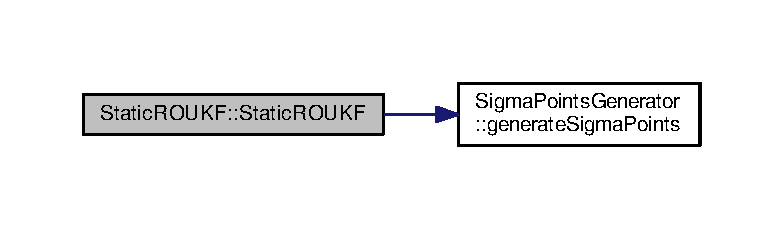
\includegraphics[width=350pt]{classStaticROUKF_ad16035ac639499eb59aee6b88ca9ca52_cgraph}
\end{center}
\end{figure}


\subsection{Member Function Documentation}
\mbox{\Hypertarget{classStaticROUKF_a60e34a2958fa111850d2e74bc85c4f64}\label{classStaticROUKF_a60e34a2958fa111850d2e74bc85c4f64}} 
\index{Static\+R\+O\+U\+KF@{Static\+R\+O\+U\+KF}!execute\+Step@{execute\+Step}}
\index{execute\+Step@{execute\+Step}!Static\+R\+O\+U\+KF@{Static\+R\+O\+U\+KF}}
\subsubsection{\texorpdfstring{execute\+Step()}{executeStep()}}
{\footnotesize\ttfamily double Static\+R\+O\+U\+K\+F\+::execute\+Step (\begin{DoxyParamCaption}\item[{double $\ast$}]{Zkhatc,  }\item[{forward\+Op}]{A,  }\item[{observation\+Op}]{H }\end{DoxyParamCaption})}

Performs one step of the Kalman filtering process in serial execution of the sigma points. 
\begin{DoxyParams}{Parameters}
{\em Zkhatc} & Current observations estimations. \\
\hline
{\em A} & Forward operator. \\
\hline
{\em H} & Observation operator; \\
\hline
\end{DoxyParams}
\begin{DoxyReturn}{Returns}
Current L2 norm of the errors across all observations. 
\end{DoxyReturn}


Definition at line 39 of file Static\+R\+O\+U\+K\+F.\+cpp.

\mbox{\Hypertarget{classStaticROUKF_a8b0b1ec67cf2f16366c628f775519baf}\label{classStaticROUKF_a8b0b1ec67cf2f16366c628f775519baf}} 
\index{Static\+R\+O\+U\+KF@{Static\+R\+O\+U\+KF}!execute\+Step\+Parallel@{execute\+Step\+Parallel}}
\index{execute\+Step\+Parallel@{execute\+Step\+Parallel}!Static\+R\+O\+U\+KF@{Static\+R\+O\+U\+KF}}
\subsubsection{\texorpdfstring{execute\+Step\+Parallel()}{executeStepParallel()}}
{\footnotesize\ttfamily double Static\+R\+O\+U\+K\+F\+::execute\+Step\+Parallel (\begin{DoxyParamCaption}\item[{double $\ast$}]{Zkhatc,  }\item[{forward\+Op}]{A,  }\item[{observation\+Op}]{H,  }\item[{int}]{seed,  }\item[{M\+P\+I\+\_\+\+Comm}]{local\+\_\+comm,  }\item[{M\+P\+I\+\_\+\+Comm}]{masters\+\_\+comm }\end{DoxyParamCaption})}

Performs one step of the Kalman filtering process with parallel execution of the sigma points. 
\begin{DoxyParams}{Parameters}
{\em Zkhatc} & Current observations estimations. \\
\hline
{\em A} & Forward operator. \\
\hline
{\em H} & Observation operator; \\
\hline
{\em seed} & Sigma point ID for the current M\+PI process. \\
\hline
{\em local\+\_\+comm} & Communicator of all M\+PI processes that solve the sigma point {\ttfamily seed}. \\
\hline
{\em masters\+\_\+comm} & Communicator of the master M\+PI processes of each sigma point {\ttfamily seed}. \\
\hline
\end{DoxyParams}
\begin{DoxyReturn}{Returns}
Current L2 norm of the errors across all observations. 
\end{DoxyReturn}


Definition at line 98 of file Static\+R\+O\+U\+K\+F.\+cpp.

\mbox{\Hypertarget{classStaticROUKF_ae51260a2b2792f27ecf3c441ebe532d4}\label{classStaticROUKF_ae51260a2b2792f27ecf3c441ebe532d4}} 
\index{Static\+R\+O\+U\+KF@{Static\+R\+O\+U\+KF}!get\+Error@{get\+Error}}
\index{get\+Error@{get\+Error}!Static\+R\+O\+U\+KF@{Static\+R\+O\+U\+KF}}
\subsubsection{\texorpdfstring{get\+Error()}{getError()}}
{\footnotesize\ttfamily void Static\+R\+O\+U\+K\+F\+::get\+Error (\begin{DoxyParamCaption}\item[{double $\ast$$\ast$}]{err }\end{DoxyParamCaption})}

Returns the error associated to each observation at the current iteration in a S\+TL array. 
\begin{DoxyParams}{Parameters}
{\em err} & Error associated to each observation at the current iteration. \\
\hline
\end{DoxyParams}


Definition at line 179 of file Static\+R\+O\+U\+K\+F.\+cpp.

\mbox{\Hypertarget{classStaticROUKF_acf22483dd4fefba60df6f5e7f29429ec}\label{classStaticROUKF_acf22483dd4fefba60df6f5e7f29429ec}} 
\index{Static\+R\+O\+U\+KF@{Static\+R\+O\+U\+KF}!get\+Obs\+Error@{get\+Obs\+Error}}
\index{get\+Obs\+Error@{get\+Obs\+Error}!Static\+R\+O\+U\+KF@{Static\+R\+O\+U\+KF}}
\subsubsection{\texorpdfstring{get\+Obs\+Error()}{getObsError()}}
{\footnotesize\ttfamily double Static\+R\+O\+U\+K\+F\+::get\+Obs\+Error (\begin{DoxyParamCaption}\item[{int}]{num\+Observation }\end{DoxyParamCaption})}

Returns the error associated to the {\ttfamily num\+Observation} observation. 
\begin{DoxyParams}{Parameters}
{\em num\+Observation} & Index of the observation of interest. \\
\hline
\end{DoxyParams}


Definition at line 183 of file Static\+R\+O\+U\+K\+F.\+cpp.

\mbox{\Hypertarget{classStaticROUKF_ae94282d13b307666494ee76aadc58aa4}\label{classStaticROUKF_ae94282d13b307666494ee76aadc58aa4}} 
\index{Static\+R\+O\+U\+KF@{Static\+R\+O\+U\+KF}!get\+Observations@{get\+Observations}}
\index{get\+Observations@{get\+Observations}!Static\+R\+O\+U\+KF@{Static\+R\+O\+U\+KF}}
\subsubsection{\texorpdfstring{get\+Observations()}{getObservations()}}
{\footnotesize\ttfamily int Static\+R\+O\+U\+K\+F\+::get\+Observations (\begin{DoxyParamCaption}{ }\end{DoxyParamCaption}) const}

Return the number of observations used in this instance of the kalman filter. \begin{DoxyReturn}{Returns}
Number of observations used in this instance of the kalman filter. 
\end{DoxyReturn}


Definition at line 230 of file Static\+R\+O\+U\+K\+F.\+cpp.

\mbox{\Hypertarget{classStaticROUKF_ac1acb518b1978a0c07bc9b8c6a1fc36a}\label{classStaticROUKF_ac1acb518b1978a0c07bc9b8c6a1fc36a}} 
\index{Static\+R\+O\+U\+KF@{Static\+R\+O\+U\+KF}!get\+Parameters@{get\+Parameters}}
\index{get\+Parameters@{get\+Parameters}!Static\+R\+O\+U\+KF@{Static\+R\+O\+U\+KF}}
\subsubsection{\texorpdfstring{get\+Parameters()}{getParameters()}}
{\footnotesize\ttfamily void Static\+R\+O\+U\+K\+F\+::get\+Parameters (\begin{DoxyParamCaption}\item[{double $\ast$$\ast$}]{ThetaC }\end{DoxyParamCaption})\hspace{0.3cm}{\ttfamily [virtual]}}

Getter of the field {\ttfamily Theta}. 
\begin{DoxyParams}{Parameters}
{\em ThetaC} & Field {\ttfamily Theta} converted to S\+TL array. \\
\hline
\end{DoxyParams}


Definition at line 171 of file Static\+R\+O\+U\+K\+F.\+cpp.

\mbox{\Hypertarget{classStaticROUKF_a5000d72faeb9a7f496ab24ae09ead1ab}\label{classStaticROUKF_a5000d72faeb9a7f496ab24ae09ead1ab}} 
\index{Static\+R\+O\+U\+KF@{Static\+R\+O\+U\+KF}!get\+Parameters\+Std@{get\+Parameters\+Std}}
\index{get\+Parameters\+Std@{get\+Parameters\+Std}!Static\+R\+O\+U\+KF@{Static\+R\+O\+U\+KF}}
\subsubsection{\texorpdfstring{get\+Parameters\+Std()}{getParametersStd()}}
{\footnotesize\ttfamily vector$<$ double $>$ Static\+R\+O\+U\+K\+F\+::get\+Parameters\+Std (\begin{DoxyParamCaption}{ }\end{DoxyParamCaption})}

Returns a vector with the standard variation of each parameter at the current iteration. \begin{DoxyReturn}{Returns}
Vector with the standard variation of each parameter at the current iteration. 
\end{DoxyReturn}


Definition at line 225 of file Static\+R\+O\+U\+K\+F.\+cpp.

\mbox{\Hypertarget{classStaticROUKF_a9896d986a5cb17d1672b3aa8ff5a806d}\label{classStaticROUKF_a9896d986a5cb17d1672b3aa8ff5a806d}} 
\index{Static\+R\+O\+U\+KF@{Static\+R\+O\+U\+KF}!get\+States@{get\+States}}
\index{get\+States@{get\+States}!Static\+R\+O\+U\+KF@{Static\+R\+O\+U\+KF}}
\subsubsection{\texorpdfstring{get\+States()}{getStates()}}
{\footnotesize\ttfamily int Static\+R\+O\+U\+K\+F\+::get\+States (\begin{DoxyParamCaption}{ }\end{DoxyParamCaption}) const}

Return the number of states used in this instance of the kalman filter. \begin{DoxyReturn}{Returns}
Number of states used in this instance of the kalman filter. 
\end{DoxyReturn}


Definition at line 235 of file Static\+R\+O\+U\+K\+F.\+cpp.

\mbox{\Hypertarget{classStaticROUKF_a2df76479be92ab63f645eb27184f9a23}\label{classStaticROUKF_a2df76479be92ab63f645eb27184f9a23}} 
\index{Static\+R\+O\+U\+KF@{Static\+R\+O\+U\+KF}!reset@{reset}}
\index{reset@{reset}!Static\+R\+O\+U\+KF@{Static\+R\+O\+U\+KF}}
\subsubsection{\texorpdfstring{reset()}{reset()}}
{\footnotesize\ttfamily void Static\+R\+O\+U\+K\+F\+::reset (\begin{DoxyParamCaption}\item[{int}]{n\+Observations,  }\item[{int}]{n\+States,  }\item[{int}]{n\+Parameters,  }\item[{double $\ast$}]{states\+Uncertainty,  }\item[{double $\ast$}]{parameters\+Uncertainty,  }\item[{\mbox{\hyperlink{classSigmaPointsGenerator_ad6f9474c0313425a10add120e0acf944}{Sigma\+Points\+Generator\+::\+S\+I\+G\+M\+A\+\_\+\+D\+I\+S\+T\+R\+I\+B\+U\+T\+I\+ON}}}]{sigma\+Distribution }\end{DoxyParamCaption})}

Returns to the initial state of the kalman filter. Not fully tested 
\begin{DoxyParams}{Parameters}
{\em n\+Observations} & Quantity of observations. \\
\hline
{\em n\+States} & Quantity of states. \\
\hline
{\em n\+Parameters} & Quantity of parameters. \\
\hline
{\em states\+Uncertainty} & Vector with the uncertainty of each state in X. \\
\hline
{\em parameters\+Uncertainty} & Vector with the uncertainty of each parameter in Theta. \\
\hline
{\em sigma\+Distribution} & Type of sigmas applied to assess the unscented transform. Only S\+I\+M\+P\+L\+EX is available by now. \\
\hline
\end{DoxyParams}


Definition at line 187 of file Static\+R\+O\+U\+K\+F.\+cpp.

Here is the call graph for this function\+:\nopagebreak
\begin{figure}[H]
\begin{center}
\leavevmode
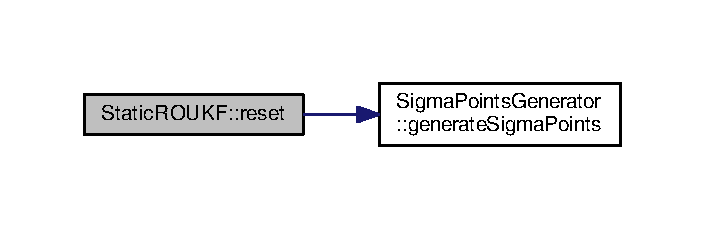
\includegraphics[width=338pt]{classStaticROUKF_a2df76479be92ab63f645eb27184f9a23_cgraph}
\end{center}
\end{figure}
\mbox{\Hypertarget{classStaticROUKF_a4588baa8e0022f23b8cd8b43f10dc74a}\label{classStaticROUKF_a4588baa8e0022f23b8cd8b43f10dc74a}} 
\index{Static\+R\+O\+U\+KF@{Static\+R\+O\+U\+KF}!set\+Parameters@{set\+Parameters}}
\index{set\+Parameters@{set\+Parameters}!Static\+R\+O\+U\+KF@{Static\+R\+O\+U\+KF}}
\subsubsection{\texorpdfstring{set\+Parameters()}{setParameters()}}
{\footnotesize\ttfamily void Static\+R\+O\+U\+K\+F\+::set\+Parameters (\begin{DoxyParamCaption}\item[{double $\ast$}]{ThetaC }\end{DoxyParamCaption})\hspace{0.3cm}{\ttfamily [virtual]}}

Setter of the field {\ttfamily Theta}. 
\begin{DoxyParams}{Parameters}
{\em ThetaC} & Array of parameters. \\
\hline
\end{DoxyParams}


Definition at line 175 of file Static\+R\+O\+U\+K\+F.\+cpp.

\mbox{\Hypertarget{classStaticROUKF_a1dda098190863474729ba15728b5943a}\label{classStaticROUKF_a1dda098190863474729ba15728b5943a}} 
\index{Static\+R\+O\+U\+KF@{Static\+R\+O\+U\+KF}!to\+String@{to\+String}}
\index{to\+String@{to\+String}!Static\+R\+O\+U\+KF@{Static\+R\+O\+U\+KF}}
\subsubsection{\texorpdfstring{to\+String()}{toString()}}
{\footnotesize\ttfamily void Static\+R\+O\+U\+K\+F\+::to\+String (\begin{DoxyParamCaption}{ }\end{DoxyParamCaption})}

Prints the private attributes of the \mbox{\hyperlink{classROUKF}{R\+O\+U\+KF}} instance. 

Definition at line 213 of file Static\+R\+O\+U\+K\+F.\+cpp.



\subsection{Member Data Documentation}
\mbox{\Hypertarget{classStaticROUKF_a8b9ab6dd1eb28ac72f1d7f0d1f7f7685}\label{classStaticROUKF_a8b9ab6dd1eb28ac72f1d7f0d1f7f7685}} 
\index{Static\+R\+O\+U\+KF@{Static\+R\+O\+U\+KF}!alpha@{alpha}}
\index{alpha@{alpha}!Static\+R\+O\+U\+KF@{Static\+R\+O\+U\+KF}}
\subsubsection{\texorpdfstring{alpha}{alpha}}
{\footnotesize\ttfamily double Static\+R\+O\+U\+K\+F\+::alpha\hspace{0.3cm}{\ttfamily [private]}}

Weight for each sigma point. 

Definition at line 62 of file Static\+R\+O\+U\+K\+F.\+h.

\mbox{\Hypertarget{classStaticROUKF_a23471ddebcf45d3d2c6a0867ac47bde3}\label{classStaticROUKF_a23471ddebcf45d3d2c6a0867ac47bde3}} 
\index{Static\+R\+O\+U\+KF@{Static\+R\+O\+U\+KF}!Dsigma@{Dsigma}}
\index{Dsigma@{Dsigma}!Static\+R\+O\+U\+KF@{Static\+R\+O\+U\+KF}}
\subsubsection{\texorpdfstring{Dsigma}{Dsigma}}
{\footnotesize\ttfamily arma\+::mat Static\+R\+O\+U\+K\+F\+::\+Dsigma\hspace{0.3cm}{\ttfamily [private]}}

Matrix with sigma points weighted as rows. 

Definition at line 48 of file Static\+R\+O\+U\+K\+F.\+h.

\mbox{\Hypertarget{classStaticROUKF_ab4f563a81a206f47c1b60e3b0e80f356}\label{classStaticROUKF_ab4f563a81a206f47c1b60e3b0e80f356}} 
\index{Static\+R\+O\+U\+KF@{Static\+R\+O\+U\+KF}!error@{error}}
\index{error@{error}!Static\+R\+O\+U\+KF@{Static\+R\+O\+U\+KF}}
\subsubsection{\texorpdfstring{error}{error}}
{\footnotesize\ttfamily arma\+::mat Static\+R\+O\+U\+K\+F\+::error\hspace{0.3cm}{\ttfamily [private]}}

Vector with the observations errors after the last iteration. 

Definition at line 53 of file Static\+R\+O\+U\+K\+F.\+h.

\mbox{\Hypertarget{classStaticROUKF_abbdca814d9577bf7b9f34264cb1f6836}\label{classStaticROUKF_abbdca814d9577bf7b9f34264cb1f6836}} 
\index{Static\+R\+O\+U\+KF@{Static\+R\+O\+U\+KF}!L\+Theta@{L\+Theta}}
\index{L\+Theta@{L\+Theta}!Static\+R\+O\+U\+KF@{Static\+R\+O\+U\+KF}}
\subsubsection{\texorpdfstring{L\+Theta}{LTheta}}
{\footnotesize\ttfamily arma\+::mat Static\+R\+O\+U\+K\+F\+::\+L\+Theta\hspace{0.3cm}{\ttfamily [private]}}

L part of the covariance matrix after LU factorization concerning to the parameter part of the extended state vector. 

Definition at line 41 of file Static\+R\+O\+U\+K\+F.\+h.

\mbox{\Hypertarget{classStaticROUKF_a3b30dbaa7706106840323888eff5f7b5}\label{classStaticROUKF_a3b30dbaa7706106840323888eff5f7b5}} 
\index{Static\+R\+O\+U\+KF@{Static\+R\+O\+U\+KF}!n\+Observations@{n\+Observations}}
\index{n\+Observations@{n\+Observations}!Static\+R\+O\+U\+KF@{Static\+R\+O\+U\+KF}}
\subsubsection{\texorpdfstring{n\+Observations}{nObservations}}
{\footnotesize\ttfamily int Static\+R\+O\+U\+K\+F\+::n\+Observations\hspace{0.3cm}{\ttfamily [private]}}

Quantity of observations. 

Definition at line 56 of file Static\+R\+O\+U\+K\+F.\+h.

\mbox{\Hypertarget{classStaticROUKF_a2b03763759259e2742eef0221a4218f7}\label{classStaticROUKF_a2b03763759259e2742eef0221a4218f7}} 
\index{Static\+R\+O\+U\+KF@{Static\+R\+O\+U\+KF}!n\+Parameters@{n\+Parameters}}
\index{n\+Parameters@{n\+Parameters}!Static\+R\+O\+U\+KF@{Static\+R\+O\+U\+KF}}
\subsubsection{\texorpdfstring{n\+Parameters}{nParameters}}
{\footnotesize\ttfamily int Static\+R\+O\+U\+K\+F\+::n\+Parameters\hspace{0.3cm}{\ttfamily [private]}}

Quantity of parameters. 

Definition at line 58 of file Static\+R\+O\+U\+K\+F.\+h.

\mbox{\Hypertarget{classStaticROUKF_ad512fa829a858c957c9fa38f45e6b1e0}\label{classStaticROUKF_ad512fa829a858c957c9fa38f45e6b1e0}} 
\index{Static\+R\+O\+U\+KF@{Static\+R\+O\+U\+KF}!n\+States@{n\+States}}
\index{n\+States@{n\+States}!Static\+R\+O\+U\+KF@{Static\+R\+O\+U\+KF}}
\subsubsection{\texorpdfstring{n\+States}{nStates}}
{\footnotesize\ttfamily int Static\+R\+O\+U\+K\+F\+::n\+States\hspace{0.3cm}{\ttfamily [private]}}

Quantity of states. 

Definition at line 60 of file Static\+R\+O\+U\+K\+F.\+h.

\mbox{\Hypertarget{classStaticROUKF_a0d0d000c613a6f83224f1e2af9c90c26}\label{classStaticROUKF_a0d0d000c613a6f83224f1e2af9c90c26}} 
\index{Static\+R\+O\+U\+KF@{Static\+R\+O\+U\+KF}!Pa@{Pa}}
\index{Pa@{Pa}!Static\+R\+O\+U\+KF@{Static\+R\+O\+U\+KF}}
\subsubsection{\texorpdfstring{Pa}{Pa}}
{\footnotesize\ttfamily arma\+::mat Static\+R\+O\+U\+K\+F\+::\+Pa\hspace{0.3cm}{\ttfamily [private]}}

Matrix {\ttfamily sigma} times {\ttfamily Dsigma} . 

Definition at line 50 of file Static\+R\+O\+U\+K\+F.\+h.

\mbox{\Hypertarget{classStaticROUKF_a135dff2733c7d15f6a481a8b09d82dce}\label{classStaticROUKF_a135dff2733c7d15f6a481a8b09d82dce}} 
\index{Static\+R\+O\+U\+KF@{Static\+R\+O\+U\+KF}!sigma@{sigma}}
\index{sigma@{sigma}!Static\+R\+O\+U\+KF@{Static\+R\+O\+U\+KF}}
\subsubsection{\texorpdfstring{sigma}{sigma}}
{\footnotesize\ttfamily arma\+::mat Static\+R\+O\+U\+K\+F\+::sigma\hspace{0.3cm}{\ttfamily [private]}}

Matrix with sigma points as columns. 

Definition at line 46 of file Static\+R\+O\+U\+K\+F.\+h.

\mbox{\Hypertarget{classStaticROUKF_a8c15ae84fa30d7663ba976f8996dd81f}\label{classStaticROUKF_a8c15ae84fa30d7663ba976f8996dd81f}} 
\index{Static\+R\+O\+U\+KF@{Static\+R\+O\+U\+KF}!Theta@{Theta}}
\index{Theta@{Theta}!Static\+R\+O\+U\+KF@{Static\+R\+O\+U\+KF}}
\subsubsection{\texorpdfstring{Theta}{Theta}}
{\footnotesize\ttfamily arma\+::mat Static\+R\+O\+U\+K\+F\+::\+Theta\hspace{0.3cm}{\ttfamily [private]}}

Parameters vector. 

Definition at line 35 of file Static\+R\+O\+U\+K\+F.\+h.

\mbox{\Hypertarget{classStaticROUKF_a58ed92ebb17443f82e2c7124287c8173}\label{classStaticROUKF_a58ed92ebb17443f82e2c7124287c8173}} 
\index{Static\+R\+O\+U\+KF@{Static\+R\+O\+U\+KF}!U@{U}}
\index{U@{U}!Static\+R\+O\+U\+KF@{Static\+R\+O\+U\+KF}}
\subsubsection{\texorpdfstring{U}{U}}
{\footnotesize\ttfamily arma\+::mat Static\+R\+O\+U\+K\+F\+::U\hspace{0.3cm}{\ttfamily [private]}}

U part of the covariance matrix after LU factorization. 

Definition at line 37 of file Static\+R\+O\+U\+K\+F.\+h.

\mbox{\Hypertarget{classStaticROUKF_a7d4e7278e9aed5a551905ce4109da072}\label{classStaticROUKF_a7d4e7278e9aed5a551905ce4109da072}} 
\index{Static\+R\+O\+U\+KF@{Static\+R\+O\+U\+KF}!U2@{U2}}
\index{U2@{U2}!Static\+R\+O\+U\+KF@{Static\+R\+O\+U\+KF}}
\subsubsection{\texorpdfstring{U2}{U2}}
{\footnotesize\ttfamily arma\+::mat Static\+R\+O\+U\+K\+F\+::\+U2\hspace{0.3cm}{\ttfamily [private]}}

U squared. 

Definition at line 39 of file Static\+R\+O\+U\+K\+F.\+h.

\mbox{\Hypertarget{classStaticROUKF_a612d1fae1853a0dba561a2557bb6d844}\label{classStaticROUKF_a612d1fae1853a0dba561a2557bb6d844}} 
\index{Static\+R\+O\+U\+KF@{Static\+R\+O\+U\+KF}!Wi@{Wi}}
\index{Wi@{Wi}!Static\+R\+O\+U\+KF@{Static\+R\+O\+U\+KF}}
\subsubsection{\texorpdfstring{Wi}{Wi}}
{\footnotesize\ttfamily arma\+::sp\+\_\+mat Static\+R\+O\+U\+K\+F\+::\+Wi\hspace{0.3cm}{\ttfamily [private]}}

Observations confidence matrix. 

Definition at line 43 of file Static\+R\+O\+U\+K\+F.\+h.



The documentation for this class was generated from the following files\+:\begin{DoxyCompactItemize}
\item 
Static\+R\+O\+U\+K\+F.\+h\item 
Static\+R\+O\+U\+K\+F.\+cpp\end{DoxyCompactItemize}

%--- End generated contents ---

% Index
\backmatter
\newpage
\phantomsection
\clearemptydoublepage
\addcontentsline{toc}{chapter}{Index}
\printindex

\end{document}
